% !TEX encoding = UTF-8 Unicode
% !TEX TS-program = pdflatex
% !TeX spellcheck = en_GB

%%%%%%% La riga soprastante serve per configurare gli editor
%%%%%%% TeXShop, TeXworks e TeXstudio per gestire questo file
%%%%%%% con la codifica UFF-8.
%%%%%%% Se si vuole usare un'altra codifica si veda sotto.
%%%%%%%

%%%%%%%  Esempio con molte opzioni
%%%%%%% Le opzioni nella forma "chiave=valore" sono definite
%%%%%%% perché la classe dalla versione 6.1.00 usa il pacchetto
%%%%%%% xkeyval. Vedere sulla documentazione in inglese o
%%%%%%% in italiano quali chiavi accettano valori.

%%%%%%% L'opzione per il corpo accetta qualsiasi valore, anche fratto
%%%%%%% (per esempio: corpo=11.5pt) e va sempre scritto con una
%%%%%%% unità di misura. L'utente è pregato di non esagerare con
%%%%%%% corpi normali minori di 9.5pt o maggiori di 13pt.
%%%%%%%
%%%%%%% Le opzioni per inputenc e fontenc vanno per prime.
%%%%%%% Vengono ignorate se NON si compone con pdfLaTeX. Ma
%%%%%%% questo è un esempio per pdfLaTeX.
%%%%%%%

\documentclass[%
cucitura,
12pt,
%twoside,
%    stile=classica,
%oldstyle,
%    autoretitolo,
tipotesi=magistrale,
%greek,
%evenboxes
numerazioneromana
]{toptesi}
%%%%%%%%%%%%%%%%%%%%%%%%%%%%%%%%%%%%%%%%%%%%%%%%%%%%
%%%%%% Per la codifica d'entratasi può scegliere quella che si vuole,
%%%%%% ma si consiglia di preferire utf8; in ogni caso non scegliere
%%%%%% codifiche specifiche del sistema operativo.

\usepackage[utf8]{inputenc}% codifica d'entrata
\usepackage[T1]{fontenc}%    codifica dei font
\usepackage{lmodern}%        scelta dei font

\usepackage{amsmath}
\usepackage{amssymb}
\usepackage{amsfonts}
\usepackage{varioref}
\usepackage{hyperref} 
\usepackage{cleveref}



% Vedere la documentazione toptesi-it.pdf per le
% attenzioni che bisogna usare al fine di ottenere un file
% veramente conforme alle norme per l'archiviabilità.


\usepackage{hyperref}

\hypersetup{%
	pdfpagemode={UseOutlines},
	bookmarksopen,
	pdfstartview={FitH},
	colorlinks,
	linkcolor={blue},
	citecolor={blue},
	urlcolor={blue}
}
% Questo è utile per evidenziare le cose "dubbie e da correggere"
% Poi si elimina il comando cosi' non restano \boh{} in giro
\newcommand{\michiardi}[1]{\textcolor{red}{(Michiardi P.) #1}}
\newcommand{\macaluso}[1]{\textcolor{red}{(Macaluso P.) #1}}

\newcommand{\todomichiardi}[1]{\textcolor{red}{TODO (Michiardi P.): #1}}
\newcommand{\todomacaluso}[1]{\textcolor{red}{TODO (Macaluso P.): #1}}


% Per scrivere testo fasullo in "latinorum"
\usepackage{lipsum}
%

%%%%%%% Definizioni locali
\newtheorem{osservazione}{Osservazione}% Standard LaTeX
\ExtendCaptions{english}{Abstract}{Acknowledgements}

\usepackage[acronym, toc]{glossaries}

\makeglossaries
% Black for all glossaries entries
\renewcommand*{\glstextformat}[1]{\textcolor{black}{#1}}
%\setacronymstyle{long-short}
\newacronym{cnn}{CNN}{Convolutional Neural Network}
\newacronym{nn}{NN}{Neural Network}
\newacronym{dl}{DL}{Deep Learning}
\newacronym{rl}{RL}{Reinforcement Learning}
\newacronym{sac}{SAC}{Soft Actor-Critic}
\newacronym{ddpg}{DDPG}{Deep Deterministic Policy Gradient}
\newacronym{iid}{i.i.d.}{indipendent and identically distributed}
\newacronym{mdp}{MDP}{Markov decision process}



\usepackage{tikz}
\usetikzlibrary{arrows,positioning}
\usetikzlibrary{calc} % for manimulation of coordinates
\tikzset{
	%Define standard arrow tip
	>=stealth',
	%Define style for boxes
	mylabel/.style={text width=7em, text centered},
	punkt/.style={
		rectangle,
		rounded corners,
		draw=black, very thick,
		text width=8em,
		minimum height=2.5em,
		text centered},
	% Define arrow style
	pil/.style={
		->,
		thick,
		shorten <=2pt,
		shorten >=2pt,}
}

\begin{document}
	\errorcontextlines=9
\english
\iflanguage{english}{%
	\retrofrontespizio{This work is subject to the Creative Commons Licence}
	% \DottoratoIn{PhD Course in\space}
	\StrutturaDidattica{Department of }
	\struttura{Control and Computer Engineering}
	\CorsoDiLaureaIn{Master of Science in\space}
	%\NomeMonografia{Bachelor Degree Final Work}
	\TesiDiLaurea{Master Thesis}
	%\NomeDissertazione{PhD Dissertation}
	%\InName{in}
	\CandidateName{Candidate}% or Candidate
	\AdvisorName{Supervisors}% or Supervisor
	\TutorName{Tutor}
	\NomeTutoreAziendale{Internship Tutor}
	%\CycleName{cycle}
	%\NomePrimoTomo{First volume}
	%\NomeSecondoTomo{Second Volume}
	%\NomeTerzoTomo{Third Volume}
	%\NomeQuartoTomo{Fourth Volume}
	%\logosede{logodue}% or comma separated list of logos
	\TitoloListaCandidati{Candidate,Candidate,Candidates,Candidates}
}{}
%%%%%%% Questi comandi è meglio metterli dentro l'ambiente
%%%%%%% frontespizio o frontespizio*, oppure in un file di
%%%%%%% configurazione personale. Si veda la documentazione
%%%%%%% inglese o italiana.
%%%%%%% Comunque i presenti comandi servono per comporre la
%%%%%%% tesi con i moduli di estensione standard del pacchetto
%%%%%%% TOPtesi.

\begin{ThesisTitlePage}
	\ateneo{Politecnico di Torino}
	\titolo{Deep Reinforcement Learning for autonomous systems}
	\sottotitolo{Designing a control system to exploit model-free deep reinforcement learning algorithms to solve a real-world autonomous driving task of a small robot.}
	%%%%%%% Corso degli studi
	\corsodilaurea{Computer Engineering (Software Career)}
	%%%%%%% L'eventuale numero di matricola va fra parentesi quadre
	\renewcommand\IDlabel{\\\quad\xspace}
	\candidato{Piero \textsc{Macaluso}}[s252894]
	%\secondocandidato{Evangelista \textsc{Torricelli}}[123457]

	%%%%%%% Relatori o supervisori
	%
	\relatore{Prof.~Pietro \textsc{Michiardi}}
	\secondorelatore{Prof.~Elena \textsc{Baralis}}

	%%%%%%% Seduta dell'esame
	%		\sedutadilaurea{\textsc{October} 2019}
	%%%%%%%% oppure:
	\sedutadilaurea{\textsc{Academic~Year} 2019-2020}% 
	%%%%%%% Logo della sede
	\logosede{logopolito}% 
\end{ThesisTitlePage}


%%%%%%% Per cambiare l'offset per la rilegatura;
%%%%%%% meno offset c'e', meglio e'
%\setbindingcorrection{3mm}

\begin{abstract}
	Because of its potential to thoroughly change mobility and transport, autonomous systems and self-driving vehicles are attracting much attention from both the research community and industry.
	Recent work has demonstrated that it is possible to rely on a comprehensive understanding of the immediate environment while following simple high-level directions, to obtain a more scalable approach that can make autonomous driving a ubiquitous technology.
	However, to date, the majority of the methods concentrates on deterministic control optimisation algorithms to select the right action, while the usage of deep learning and machine learning is entirely dedicated to object detection and recognition.

	Recently, we have witnessed a remarkable increase in interest in Reinforcement Learning (RL). It is a machine learning field focused on solving Markov Decision Processes (MDP), where an agent learns to make decisions by mapping situations and actions according to the information it gathers from the surrounding environment and from the reward it receives, trying to maximise it.
	As researchers discovered, it can be surprisingly useful to solve tasks in simulated environments like games and computer games, and it showed encouraging performance in tasks with robotic manipulators. Furthermore, the great fervour produced by the widespread exploitation of deep learning opened the doors to function approximation with convolutional neural networks, developing what is nowadays known as deep reinforcement learning.

	In this thesis, we argue that the generality of reinforcement learning makes it a useful framework where to apply autonomous driving to inject artificial intelligence not only in the detection component but also in the decision-making one.
	The focus of the majority of reinforcement learning projects is on a simulated environment. However, a more challenging approach of reinforcement learning consists of the application of this type of algorithms in the real world.
	For this reason, we designed and implemented a control system for Cozmo, a small toy robot developed by Anki company, by exploiting the Cozmo SDK, PyTorch and OpenAI Gym to build up a standardised environment in which to apply any reinforcement learning algorithm: it represents the first contribution of our thesis.

	Furthermore, we designed a circuit where we were able to carry out experiments in the real world, the second contribution of our work.
	We started from a simplified environment where to test algorithm functionalities to motivate and discuss our implementation choices.
	Therefore, we implemented our version of Soft Actor-Critic (SAC), a model-free reinforcement learning algorithm suitable for real-world experiments, to solve the specific self-driving task with Cozmo. The agent managed to reach a maximum value of above 3.5 meters in the testing phase, which equals more than one complete tour of the track. Despite this significant result, it was not able to learn how to drive securely and stably. Thus, we focused on the analysis of the strengths and weaknesses of this approach outlining what could be the next steps to make this cutting-edge technology concrete and efficient.

\end{abstract}

% \paginavuota % funziona anche senza specificare l'opzione classica

%\printglossaries

% \ringraziamenti

% \todomacaluso{Acknowledgements must be prepared!}

\tablespagetrue\figurespagetrue % normalmente questa riga non serve ed e' commentata
\indici

%%%%%%%% Altro esperimento con l'opzione classica
%%%%%%%% Non usare mai anche se qui lo si è fatto!
%%%%%%%% Oltretutto funziona solo se si è specificata la lingua greca fra le opzioni.
%%%%%%%% Commentare fra \ifclassica fino a \fi compresi. 
%\ifclassica
%	\begin{citazioni}
%		\textit{testo testo testo\\testo testo testo}
%
%		[\textsc{G.\ Leopardi}, Operette Morali]\vspace{1em}
%
%		\textgreek{>all'a p'anta <o k'eraunos d'' >oiak'izei}
%
%		[\textsc{Eraclito}, fr.\ D-K 134]
%	\end{citazioni}

%\fi
%%%%%%%% fine esperimento

	\mainmatter
	\chapter{Introduction}

\todomacaluso{Da rifare totalmente alla fine}

\section{Motivation}

Autonomous systems, and in particular self-driving for unsupervised robots and vehicles (e.g.\ self-driving cars) is a topic that has attracted a lot of attention from both the research community and industry, due to its potential to radically change mobility and transport. In general, most approaches to date focus on formal logic methods, which define driving behavior in annotated geometric maps. This can be difficult to scale, as it relies heavily on an external mapping infrastructure rather than using and understanding the local scene.

In order to make autonomous driving a truly ubiquitous technology, in this thesis we focus on systems which address the ability to drive and navigate in the absence of maps and explicit rules, relying – just like humans do – on a comprehensive understanding of the immediate environment while following simple high-level directions (e.g.\ turn-by-turn route commands). Recent work in this area has demonstrated that this is possible on rural country roads, using GPS for coarse localization and LIDAR to understand the local scene. 

Recently, \gls{rl} – a machine learning subfield focused on solving \gls{mdp}, where an agent learns to select actions in an environment in an attempt to maximize some reward function – has been shown to achieve super-human results at games such as Go or chess, to be particularly suited for simulated environments like computer games, and to be a promising methodology for simple tasks with robotic manipulators.

In this thesis, we argue that the generality of \gls{rl} makes it a useful framework to apply to autonomous driving. 
For this reason we design and implement a control system for an autonomous driving task with a small robot, exploiting state-of-the-art model-free Deep \gls{rl} algorithms and discussing possible ways to make them data efficient.

\section{Related Work}

\section{Structure of the thesis}
The aim of this section is to describe the main structure of the thesis.

\subsubsection*{Chapter 1 - Introduction} The current chapter contains the motivation of this work and the structure of the thesis.

\subsubsection*{Chapter 2 - Reinforcement Learning Fundamentals}
The aim of this chapter is to present a description as detailed as possible about \gls{rl} state-of-the-art in order to provide the reader with useful tools to enter in this research field.
\todomacaluso{Da qui in poi questo capitolo è da fare}
\subsubsection*{Chapter 3 - Tools and Frameworks} 
This chapter explains briefly what are the main tools, frameworks and languages used in the thesis.
\todomacaluso{Continue this list}
\begin{description}
	\item[OpenAI Gym] framework for developing and comparing Reinforcement Learning algorithms and environments using standardize interface.
	\item [Anki Cozmo] it looks like a simple toy at first sight, but it hides an infinite potential under the hood, which make it a perfect candidate for the purposes of this thesis.
\end{description}

\subsubsection*{Chapter 4 - Design of the control system}

\subsubsection*{Chapter 5 - Algorithms for Autonomous Systems} 


\subsubsection*{Chapter 5 - Experiments} 
This is the most important chapter. It shows all the results obtained during the numerous experiments with comments and speculations about them.

\subsubsection*{Chapter 6 - Conclusions} 
A summary of the results obtained from experiments with a specific part dedicated to future improvements.
	\chapter{Introduction} \label{ch:ch1}

Autonomous systems and in particular self-driving for unsupervised robots and vehicles (e.g.\ self-driving cars) are becoming more and more an integral part of human lives.
This topic attracted much attention from both the research community and industry, due to its potential to radically change mobility and transport.
In general, most approaches to date focus on formal logic methods, which define driving behaviour in annotated geometric maps.
These methods can be challenging to scale, as they rely heavily on an external mapping infrastructure rather than using and understanding the local scene, leaving fully autonomous driving in a real urban environment an essential but elusive goal.

However, recent work on autonomous driving has demonstrated that it is possible to exploit the knowledge about the surrounding environment to obtain a more scalable method for self-driving vehicles.
The work in \cite{ort2018autonomous} demonstrated that this approach is feasible on rural country roads, using GPS for coarse localisation and LIDAR to understand the local scene.
The ability to drive and navigate in the absence of maps and explicit rules, relying – just like humans do – on a comprehensive understanding of the immediate environment while following simple high-level directions (e.g.\ turn-by-turn route commands) may be the correct approach to revolutionise autonomous driving by making it a genuinely ubiquitous technology.

To date, the majority of the methods adopted to exploit the local scene and to learn how to drive concentrates on deterministic algorithms to recognise the surroundings and select the right action (e.g.\ lane following problem on well-marked structured highways).
However, these methods, like the previous ones, are not able to generalise proficiently in a different environment because of their deterministic nature.

In this context, the usage of deep learning and machine learning is entirely dedicated to object detection and recognition, while the decision-making aspect is left to control optimisation algorithms \cite{huval2015empirical}.

Recently, we have witnessed a remarkable increase in interest in Reinforcement Learning (RL).
Reinforcement Learning is a machine learning field focused on solving Markov Decision Processes (MDP), where an agent learns to act in an environment by mapping situations and actions, trying to maximise some reward function.
To date, it represents the closest example of a learning approach that mimics the ability of humans to learn from experiences.
The agent, the brain of reinforcement learning, learns to make decisions according to the information it receives from the surrounding environment and from the positive (or negative) reward it receives.
It represents a crucial step towards Artificial General Intelligence (AGI).
This machine learning paradigm achieved super-human results at games such as Go \cite{silver2016mastering} or chess \cite{silver2017mastering}.
Therefore, researchers found out that it can be surprisingly useful to solve tasks in simulated environments like computer games \cite{mnih2013playing}, and it possesses promising features to perform tasks with robotic manipulators \cite{gu2017deep}.
Furthermore, the great fervour produced by the widespread exploitation of deep learning opened the doors to function approximation with neural networks and convolutional neural networks, developing what is nowadays known as Deep Reinforcement Learning.

In this thesis, we argue that the generality of reinforcement learning makes it a useful framework where to apply autonomous driving to inject artificial intelligence not only in the detection component but also in the decision-making one.
The majority of the work in this research field are focused on simulated environments where experiments with a large number of iterations can be straightforwardly completed without direct human interaction.
However, to date, the more challenging approach of reinforcement learning consists of the application of this type of algorithms in the real world \cite{kendall2019nowisthetime}.
In this context, the crucial challenges are the one related to hyper-parameters configurations that requires numerous and expensive iterations in order to obtain valuable results, but also the data noisiness and exploration.
Despite these obstacles, the results that could derive from the application of these technologies to a real context could be compelling and revolutionary.
For this reason, we accepted this challenge, and we decided to apply reinforcement learning algorithms to an autonomous driving problem, following the inspiring research of \cite{kendall2018learning}.

To develop our considerations about the particular application of this research field, we designed and implemented a control system to control Cozmo, a small toy robot developed by Anki company, by exploiting the Cozmo SDK and OpenAI Gym to build up a standardised environment in which to apply any reinforcement learning algorithm.
This implementation represents the first contribution of our thesis.
In the second contribution of our work, we aimed to implement state-of-the-art model-free deep reinforcement learning algorithms and discuss the result obtained.
We opted for Soft Actor-Critic (SAC) \cite{haarnoja2018alg,haarnoja2018soft}, a model-free reinforcement learning algorithm suitable for real-world experiments whose authors managed to overcame hyper-parameters configuration dependency of Deep Deterministic Policy Gradient (DDPG) \cite{lillicrap2015continuous}, focusing on what could be next steps to make this cutting-edge technology concrete and efficient.

\section{Structure of the thesis}

This section aims to describe the main structure of the thesis.

\subsubsection*{Chapter 1 - Introduction}

The current chapter contains the motivation underlying this work and the structure of the thesis.

\subsubsection*{Chapter 2 - Reinforcement Learning}

This chapter aims to offer a description as detailed as possible about reinforcement learning state-of-the-art in order to provide the reader with useful tools to enter in this research field.
The chapter consists of three principal parts.
The first one aims to describe traditional reinforcement learning fundamentals.
In contrast, the second one focuses reader's attention to the \textit{deep} approach to reinforcement learning, providing an outline of deep learning and presenting Deep Deterministic Policy Gradient (DDPG) and Soft Actor-Critic (SAC) algorithms.

The last part of this chapter contains a related work review to introduce to the reader the problem we aimed to solve.

\subsubsection*{Chapter 3 - Tools and Frameworks} 

This chapter explains which are the primary tools, frameworks and languages that we used in this thesis.
There will be a particular focus on \textit{OpenAI Gym}, one of the most popular reinforcement learning framework nowadays, \textit{Anki Cozmo}, the robot we used to carry out reinforcement learning experiments, and \textit{PyTorch}, the deep learning framework we used to use convolutional neural networks in reinforcement learning.

Furthermore, we outlined the motivations behind the choices made through the analysis of the alternatives present at the time of the thesis development.

\subsubsection*{Chapter 4 - Design of the control system}

The first contribution of our thesis was the implementation of a control system to perform reinforcement learning experiments in the real world, binding all the technologies presented in the previous chapter and focusing on reusability of this system to exploit other reinforcement learning algorithms.

The fourth chapter aims to present the whole set of features we implemented together with an analysis of the solutions we proposed to the problems we faced.

\subsubsection*{Chapter 5 - Experimental results} 

The second contribution of our thesis consists of the experiments we carried out with Soft Actor-Critic (SAC) algorithm to solve an autonomous driving task in the real world with Anki Cozmo robot.
This chapter aims to present the results we obtained starting from the preliminary experiments on a modified environment to tests features and functionalities and concluding the chapter with the discussion about the learning process of the robot.

It also contains some considerations about the approach taken and a general discussion on how to measure performances in reinforcement learning algorithms.

\subsubsection*{Chapter 6 - Conclusions} 

This chapter provides a summary of the results obtained from experiments together with a specific critic part.
Furthermore, the thesis will conclude with a specific part dedicated to possible future improvements to this work.

\section{Github Repository}

The work, the ideas and the source code of the work contained in this thesis is publicly available on Github at \href{https://github.com/pieromacaluso/Deep-RL-Autonomous-Systems}{\texttt{https://github.com/pieromacaluso/Deep-RL- Autonomous-Systems}}. The primary motivation behind this choice is allowing people to use, test, contribute and improve it even after the conclusion of this thesis work.

	
\chapter{Reinforcement Learning}

\acrfull{rl} is a field of Machine Learning that is experiencing a period of great fervour in the world of research, fomented by recent progress in \acrfull{dl}. This event opened the doors to function approximation with \acrfull{nn} and \acrfull{cnn} developing what is nowadays known as Deep Reinforcement Learning (Deep RL).

\acrshort{rl} represents the third paradigm of Machine Learning alongside supervised and unsupervised learning. The idea underlying this research field is that the learning process to solve a decision-making problem consists in a sequence of trial and error where the \textit{agent}, the protagonist of \acrshort{rl}, could discover and discriminate valuable decisions from penalising ones exploiting information given by a \textit{reward signal}. This interaction has a strong correlation with what human beings and animals do in the real world to forge their behaviour.

Recently \acrshort{rl} has known a remarkable development and interests in video games: it managed to beat world champions at the game of Go \cite{silver2016mastering} and Dota with superhuman results and to master numerous Atari video games \cite{mnih2013playing} from raw pixels. Decisions, actions and consequences make video games a simulated reality on which to exploit and test the power of \acrshort{rl} algorithms.
It is essential to realise that the heart of \acrshort{rl} is the science of decision making. This fact makes it compelling and general for many research fields ranging from Engineering, Computer Science, Mathematics, Economics, to Psychology and Neuroscience.

Before discussing the results of this thesis, it is good to clarify everything that today represents the state-of-the-art in order to understand the universe behind this new paradigm better. Indeed, the exploration of this field of research is the main aim of this chapter: the first section begins with the definition of the notation used and with the theoretical foundations behind \acrshort{rl}, then in the second section it moves  progressively towards what is Deep \acrshort{rl} through a careful discussion of the most essential algorithms paying more attention to those used during the thesis project.

The elaboration of this chapter is inspired by \cite{silver2015lectures}, \cite{sutton2018reinforcement}, \cite{openai2018spinningup}, \cite{lapan2018deep} and \cite{franccois2018introduction}.

\section{Fundamentals of reinforcement learning} \label{fundreinflearn}

%\todomacaluso{
%	\begin{itemize}
%		\item Introduction
%		\item Central concepts regarding fundamentals (e.g. Agent, Environment, Reward, Return)
%		\item Markov Decision Process (MDP)
%		\item Model-based prevision and control: just a brief introduction to Dynamic Programming and Policy/Value Iteration
%		\item Model-free prevision and control: a brief introduction to Monte Carlo and TD Learning approaches (SARSA and Q-Learning)
%	\end{itemize}	
%}

Reinforcement Learning is a computational approach to Sequential Decision Making. It provides a framework that is exploitable with decision-making problems that are unsolvable with a single action and need a sequence of actions, a broader horizon, to be solved. 

This section aims to present the fundamental ideas and notions behind this research field in order to help the reader to develop a baseline useful to approach \vref{deepreinflearn} about Deep Reinforcement Learning.

\subsection{The reinforcement learning problem}


The primary purpose of \acrshort{rl} algorithms is to learn how to improve and maximise a future reward by relying on interactions between two main components: the agent and the environment. 

The \textit{agent} is the entity that interacts with the environment by making decisions based on what it can observe from the state of the surrounding situation. The decisions taken by the agent consist of \textit{actions} ($a_t$).  The agent has no control over the environment, but actions are the only means by which it can modify and influence the environment.

Usually, the agent has a set of actions it can take, which is called \textit{action space}.
Some environments have discrete action spaces, where only a finite number of moves are available (e.g. $\mathcal{A} = [\text{North}, \text{South}, \text{East}, \text{West}]$ choosing the direction to take in a bidimensional maze). On the other side, there are continuous action spaces where actions are vectors of real values.
This distinction is fundamental to choose the right algorithm to use because not all of them could be compatible with both types: according to the needs of the specific case, it may be necessary to modify the algorithm to make it compatible.

The \textit{environment} represents all the things that are outside the agent. At every action received by the agent, it emits a reward, an essential aspect of \acrshort{rl}, and an observation of the environment.

The \textit{reward} $r_t$ is a scalar feedback signal that defines the objective of the \acrshort{rl} problem. This signal allows the agent to be able to distinguish positive actions from negative ones in order to reinforce and improve its behaviour. It is crucial to notice that the reward is local: it describes only the value of the latest action. Furthermore, actions may have long term consequences, delaying the reward. As it happens with human beings' decisions, receiving a conspicuous reward at a specific time step does not exclude the possibility to receive a small reward immediately afterwards and sometimes it may be better to sacrifice immediate reward to gain more rewards later.

In this context, many features make \acrshort{rl} different from supervised and unsupervised learning.
Firstly, there is no supervisor: when the agent has to decide what action to take, there is no entity that can tell him what the optimal decision is in that specific moment. The agent receives only a reward signal which may delay compared to the moment in which it has to perform the next action. 
This fact brings out another significant difference: the importance of time. The sequentiality links all actions taken by the agent, making resulting data no more \acrfull{iid}.

Given these definitions, it is noticeable that the primary purpose of the agent is to maximise the cumulative reward called \textit{return}.

The \textit{return $g_t$} is the total discounted reward starting from timestep $t$ defined by \vref{eq:return} where $\gamma$ is a \textit{discount factor}.

\begin{equation} \label{eq:return} 
	g_t = r_{t+1} + \gamma r_{t+2} + \dots = \sum_{k=0}^{\infty} \gamma^k r_{t+k+1}, \;\;\;\gamma \in [0,1)
\end{equation}

 Not only the fact that animal and human behaviour show a preference for immediate rewards rather than for the future ones motivates the presence of this factor, but it is also mathematically necessary: an infinite-horizon sum of rewards may not converge to a finite value. Indeed, the return function is a geometric series, so, if $\gamma \in [0,1)$, the series converges to a finite value equal to $1/(1-\gamma)$. For the same convergence sake, the case with $\gamma = 1$ makes sense only with a finite-horizon cumulative discounted reward.

The other data emitted by the environment is the \textit{observation} ($o_t$) that is related to the \textit{state} ($s_t$). It represents a summary of information that the agent uses to select the next action, while the \textit{state} is a function of the \textit{history} the sequence of observation, actions and rewards at timestep $t$ as shown in \vref{eq:history}.

\begin{equation}\label{eq:history}
h_t = o_1, r_1, a_1, \dots, a_{t-1}, o_{t}, r_t, \;\;\;\;\; s_t = f(h_t)
\end{equation}

The sequence of states and actions is named \textit{trajectory} ($\tau$): it is helpful to represent an episode in \acrfull{rl} framework.

The state described above is also called \textit{agent state} $s_t^a$, while the private state of the environment is called \textit{environment state} $s_t^e$. This distinction is useful for distinguishing fully observable environments where $o_t = s_t^e = s_t^a$, from partially observable environments where $s_t^e \neq s_t^a$.
In the first case, the agent can observe the environment state directly, while in the second one, it has access to partial information about the state of the environment.

Beyond the fact that this chapter will focus on fully observable environments, the distinction between state and observation is often unclear and, conventionally, the input of the agent is composed by the reward and the state as shown in \vref{fig:interactionsAE}.
\begin{figure}
	\centering
	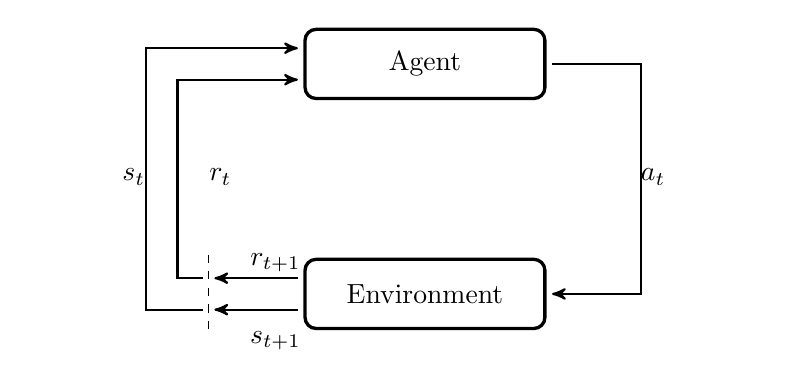
\begin{tikzpicture}
	% node Agent
	\node[punkt] (agent) {Agent};
	% node Environment
	\node[punkt, below=2cm of agent] (env) {Environment};
	% node a_t
	\node[mylabel, below right=0.75cm and 0cm of agent] (action) {$a_t$};
	% node s_t
	\node[mylabel, below left=0.75cm and 0.8cm of agent] (state) {$s_t$};
	% node r_t
	\node[mylabel, below left=0.75cm and -0.3cm of agent] (reward) {$r_t$};
	% node s_t+1
	\node[mylabel, above left=-1.3cm and -1cm of env] (state) {$s_{t+1}$};
	% node r_t+1
	\node[mylabel,above left=-.3cm and -1cm of env] (reward1) {$r_{t+1}$};
	
	
	
	\draw[pil]   (agent.east) -- ($(agent.east) + (1.2cm,0cm)$)  |-  (env.east);
	\draw[pil]   ($(env.west) + (0,-0.2cm)$) -- ($(env.west) + (-1.2cm,-0.2cm)$);
	\draw[pil]   ($(env.west) + (-1.2cm,-0.2cm)$) -- ($(env.west) + (-2cm,-0.2cm)$) |-($(agent.west) + (0,0.2cm)$);
	\draw[pil]   ($(env.west) + (0,+0.2cm)$) -- ($(env.west) + (-1.2cm,+0.2cm)$);
	\draw[pil]   ($(env.west) + (-1.2cm,+0.2cm)$) -- ($(env.west) + (-1.6cm,+0.2cm)$) |-($(agent.west) + (0,-0.2cm)$);
	\draw[dashed]  ($(env.west) - (1.2cm,-0.5cm)$) -- ($(env.west) - (1.2cm,0.5cm)$);
	\end{tikzpicture}
	\caption[Interaction loop between Agent and Environment]{Interaction loop between Agent and Environment. The reward and the state resulting from taking an action become the input of the next iteration.}
	\label{fig:interactionsAE}
\end{figure}

Furthermore, a state is called \textit{informational state} (or \textit{Markov state}) when it contains all data and information about its history. Formally, a state is a Markov state if and only if satisfies \vref{eq:markov_state}.
\begin{equation} \label{eq:markov_state}
	\mathbb{P}[s_{t+1}| s_t] = \mathbb{P}[s_{t+1} | s_1, \dots, s_t]
\end{equation}

 It means that the state contains all data and information the agent needs to know to make decisions: the whole history is not useful anymore because it is inside the state. The environment state $s_t^e$ is a Markov state.
 
 With all the definitions shown so far, it is possible to formalise the type of problems on which \acrshort{rl} can unleash all its features: the \acrfull{mdp}, a mathematic framework to model decision processes. Its main application fields are optimization and dynamic programming.
 
 An \acrshort{mdp} is defined by 
 \begin{equation}\label{eq:mdp}
 \begin{gathered} 
 <\mathcal{S}, \mathcal{A}, \mathcal{P}, \mathcal{R}, \gamma>\\
 \begin{aligned}
 	\text{where}\hspace{10pt} \mathcal{S} & \text{ is a finite set of states} \\
 	\mathcal{A} & \text{ a finite set of actions} \\
 	\mathcal{P} & \text{ a state transition probability matrix}\;\;
 	 \mathcal{P}_{ss'}^a = \mathbb{P}[s_{t+1}= s' | s_t = s, a_t = a]\\
 	\mathcal{R} & \text{ a reward function}
 	 	\;\; \mathcal{R}_{s}^a = \mathbb{E}[r_{t+1} | s_t = s, a_t = a] \\
 	 \gamma & \text{ a discount factor such that } \gamma \in [0,1]
 \end{aligned}
 \end{gathered}
 \end{equation}


The main goal of an \acrshort{mdp} is to select the best action to take, given a state, in order to collect the best reward. 

In this quick overview of the central unit of \acrshort{rl}, the components that may compose the agent, the brain of the \acrshort{rl} problem can not be missing: they are the \textit{model}, the \textit{policy} and the \textit{value function}.

A \textit{model} consist of information about the environment. These data must not be confused with the ones provided by \textit{states} and \textit{observations}: they make it possible to infer prior knowledge about the environment, influencing the behaviour of the agent.

A \textit{policy} is the core of \acrshort{rl} because it is the representation of the agent's behaviour. It is a function that describes the mapping from states to actions.  The \textit{policy} is represented by $\pi$ and it may be deterministic  $a_t = \pi(s_t)$  or stochastic $\pi(a_t|s_t) = \mathbb{P}[a_t | s_t]$.

In this perspective, it is evident that the central goal of RL is to learn an optimal policy $\pi^*$. The optimal policy is a policy which can show to the agent what the most profitable way to achieve the maximum return is, what is the best action to do in a specific situation. In order to learn the nature of the optimal policy, \acrshort{rl} exploits value functions.

A \textit{value function} represents what is the expected reward that the agent can presume to collect in the future, starting from the current state. The reward signal represents only a local value of the reward, while the value function provides a broader view of future rewards: it is a sort of prediction of rewards.

It is possible to delineate two main value functions: the \textit{state value} function and the \textit{action value} function.

\begin{itemize}
	\item The \textit{State Value Function} $V^\pi(s)$ is the expected return starting from the state $s$ and always acting according to policy $\pi$.
	\begin{equation} \label{eq:statevalue}
		V^\pi(s) = \mathbb{E}_{\tau \sim \pi}[g_t | s_0 = s]
	\end{equation}
	\item The \textit{Action Value Function} $Q^\pi(s)$ is the expected return starting from the state $s$, taking an action $a$ and then always acting according to policy $\pi$.
	\begin{equation} \label{eq:actionvalue}
	Q^\pi(s, a) = \mathbb{E}_{\tau \sim \pi}[g_t | s_0 = s, a_0 = a]
	\end{equation}
\end{itemize}


\subsection{Bellman Equations}

Both \vref{eq:statevalue,eq:actionvalue} satisfy recursive relationships between the value of a state and the values of its successor states. It is possible to see this property deriving \textit{Bellman equations} \cite{bellman2015applied} -- shown in \vref{eq:bellman} and demonstrated in \vref{appendix:bellmaneq} -- where $s_{t+1}\sim \mathit{E}$ means that the next state is sampled from the environment $E$ and $a_{t+1}\sim \pi$ shows that the policy $\pi$ determines the next action.
\begin{align} \label{eq:bellman}
	\begin{split}
V^\pi(s_t) &= \mathbb{E}_{a_t \sim \pi, s_{t+1} \sim E}[r(s_t, a_t) + \gamma V^\pi(s_{t+1})] \\
		&= \sum_{a \in \mathcal{A}}\pi(a|s)\sum_{s' \in \mathcal{S}, r \in \mathcal{R}}P(s', r | s, a)\big[r + \gamma V^\pi(s')\big]\\
Q^\pi(s_t,a_t) &= \mathbb{E}_{s_{t+1} \sim E}[r(s_t, a_t) + \gamma \mathbb{E}_{ a_{t+1} \sim \pi}[Q^\pi(s_{t+1}, a_{t+1})]]\\
	&= \sum_{a \in \mathcal{A}}\pi(a|s)\sum_{s' \in \mathcal{S}, r \in \mathcal{R}}P(s', r | s, a)\big[r + \gamma Q^\pi(s',a')\big]\\
\end{split}
\end{align}
 $r(s_t, a_t)$ is a placeholder function to represent the reward given the starting state and the action taken.
As discussed above, the goal is to find the optimal policy $\pi^*$ to exploit. It can be done using \textit{Bellman optimality equations} defined in \vref{eq:optbellman}. 
\begin{align} \label{eq:optbellman}
\begin{split}
V^*(s_t) &= \max_{a} \mathbb{E}_{s_{t+1} \sim E}[r(s_t, a) + \gamma V^*(s_{t+1})] \\
		&= \max_{a}\sum_{s' \in \mathcal{S}, r \in \mathcal{R}}P(s', r | s, a)\big[r + \gamma V^*(s')\big]\\
Q^*(s_t,a_t) &= \mathbb{E}_{s_{t+1} \sim E}[r(s_t, a_t) + \gamma \max_{a'}[Q^*(s_{t+1}, a')]]\\
			&= \sum_{s' \in \mathcal{S}, r \in \mathcal{R}}P(s', r | s, a)\big[r + \gamma \max_{a'} Q^*(s',a')\big]\\
\end{split}
\end{align}

Therefore, value functions allow defining a partial ordering over policies such that \[\pi \ge \pi' \text{ if } V_\pi \ge V_{\pi'},\forall s \in \mathcal{S}\]
This definition is helpful to enounce the \textit{Sanity Theorem}. It asserts that for any \acrshort{mdp} there exists an optimal policy $\pi^*$ that is better than or equal to all other policies, $\pi^* \ge \pi, \forall \pi$, but also that all optimal policies achieve the optimal state value function and the optimal action-value function.

%The solution of Bellman Optimality Equation is not linear and, in general, there is no closed-form solution. For this reason, there are many iterative methods.
%\todomacaluso{Bisognerà aggiungere riferimento a sezioni successive}.


\subsection{Approaches to Reinforcement Learning} \label{approaches}

Every agent consists of an RL algorithm that it exploits to maximise the reward it receives from the environment. Every single algorithm has its singularity, and it could work with a specific application field which depends on the particular approach it supports. Understanding differences among these groups is useful to adequately understand what type of algorithm satisfies better the needs of a specific problem. Nowadays, RL algorithms are numerous, and drawing the complete picture behind them could be a complicated purpose. The distinctions presented in this section aims to describe the most crucial distinctions that are useful in the context of the thesis without claiming to be exhaustive.

\subsubsection{Components of learning}

The first worthy distinction between RL algorithms can be made analysing how the algorithms exploit the different components of the agent: indeed it is possible to explain the main strategies in RL using \textit{policy}, \textit{model} and \textit{value function} defined previously.


One of the most crucial aspects of an RL algorithm is the question of whether the agent has access to or learns a model of the environment. A model of the environment enables the agent to predict state transitions and rewards.
A method is \textit{model-free} when it does not exploit the model of the environment to solve the problem. All the actions made by the agent results from direct observation of the current situation in which the agent is. It takes the observation, does computations on them and then select the best action to take.
This last representation is in contrast with \textit{model-based} methods. In this case, the agent tries to build a model of the surrounding environment in order to infer information useful to predict what the next observation or reward would be.

Both groups of methods have strong and weak sides.
Ordinarily, \textit{model-based} methods show their potential in a deterministic environment (e.g. board game with rules). In these contexts, the presence of the model enables the agent to plan by reasoning ahead, to recognise what would result from a specific decision before taking action. The agent can extract all this knowledge and learn an optimal policy to follow. However, this opportunity is not always achievable: the model may be partially or entirely unavailable, and the agent would have to learn the model from its experience. Learning a model is radically complex and may lead to various hurdles to overcome: for instance, the agent can exploit the bias present in the model, producing an agent which is not able to generalise in real environments.
On the other hand, model-free methods tend to be more straightforward to train and tune because it is usually hard to build models of a heterogeneous environment. Furthermore, model-free methods are more popular and have been more extensively developed and tested than model-based methods.

The use of policy or value function as the central part of the method represents another essential distinction between RL algorithms.
The approximation of the policy of the agent is the base of \textit{policy-based} methods. The representation of the policy is usually a probability distribution over available actions. This method points to optimise the behaviour of the agent directly and, because of its on-policy nature, may ask manifold observations from the environment: this fact makes this method not so sample-efficient.
On the opposite side, methods could be \textit{value-based}. In this case, the agent is still involved in finding the optimal behaviour to follow, but indirectly. It is not interested anymore about the probability distribution of actions. Its main objective is to determine the value of all actions available, choosing the best value. The main difference from the policy-based method is that this method can benefit from other sources, such as old policy data or replay buffer.

\begin{figure}
	\centering
	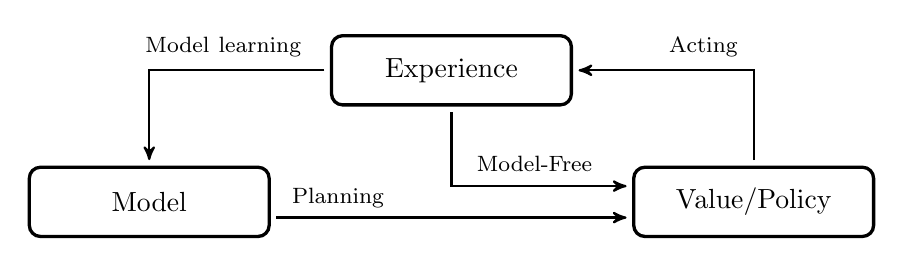
\begin{tikzpicture}
	% node Agent
	\node[punkt] (experience) {Experience};
	% node Environment
	\node[punkt, below left=0.75cm and 0.75cm of experience] (model) {Model};
	% node Value/Policy
	\node[punkt, below right=0.75cm and 0.75cm of experience] (valpol) {Value/Policy};
	\node[mylabel, above left=0.05cm and 0.00cm of experience.west] (ml) {\footnotesize Model learning};
	\node[mylabel, above right=0.05cm and 0.3cm of experience.east] (a) {\footnotesize Acting};
	\node[mylabel, below right=0.5cm and -0.3cm of experience.south] (a) {\footnotesize Model-Free};
	\node[mylabel, above right=-0.2cm and -0.5cm of model.east] (a) {\footnotesize Planning};
	\draw[pil]   (experience.south) -- ($(experience.south) - (0cm,1cm)$)  |-  ($(valpol.west) + (0cm,0.2cm)$);
	\draw[pil]   (experience.west)  -| (model.north);
	\draw[pil]   (valpol.north) -- ($(valpol.north) + (0cm,1cm)$)  |-  (experience.east);
	\draw[pil]   ($(model.east) - (0cm,0.2cm)$)  --  ($(valpol.west) - (0cm,0.2cm)$);
	\end{tikzpicture}
	\caption[Overview of different components in learning]{\small Overview of components of an agent with their relation in respect of different approaches of learning. Model-Free methods works with the experience, value functions and the policy, while model-based techniques tries to build up a model to derive value functions and policy to act in the environment.}
	\label{fig:components}
\end{figure}

\subsubsection{Learning settings}

The learning setting could be \textit{online} or \textit{offline}. In the first case, the learning process is done in parallel or concurrently while the agent continues to gather new information to use, while the second one progresses toward learning using limited data.
Generalization becomes an important problem in the last approach because the agent is not able to interact anymore with the environment.
In the context of this thesis, what matters is \textit{online learning}: in this context, the learning phase is not bound to already gathered data, but the whole process goes on using both old data coming from replay buffers and brand new data obtained in the most recent episode.

Another important difference in RL algorithms consists of the distinctive usage of the policy to learn.
On-policy algorithms profoundly depend on the training data sampled according to the current policy, because they are designed to use only data gathered with the last learned policy.
On the other hand, an off-policy method can use a different source of valuable data for the learning process instead of direct experience. This feature allows the agent to use, for instance, large experience buffers of past episodes. In this context, these buffers are usually randomly sampled in order to make the data closer to being independent and identically distributed (i.i.d): random extraction guarantees this fact.


\subsection{Dynamic Programming}

Dynamic programming (DP) \cite[Chapter 4]{sutton2018reinforcement} is one of the approaches used to solve \acrshort{rl} problems calculation the optimal policy $\pi^*$. Formally, it is a general method to solve complex problems by breaking them into sub-problems that are more convenient to solve. After solving all sub-problems, it is possible to sum them up in order to obtain the final solution to the whole original problem.

This technique provides a practical framework to solve MDP problems and to observe what is the best result achievable from it, but it assumes to have full knowledge about the specific problem. For this reason, it applies primarily to model-based problems.

Furthermore, dynamic programming methods bootstrap: it means that these strategies use one or more estimated values in the update step for the same kind of estimated value, leading to results more sensitive to initial values.

\subsubsection{Policy Iteration}

The \textit{policy iteration} aims to find the optimal policy by directly manipulating the starting policy. However, before proceeding with this process, a proper evaluation of the current policy is essential. This procedure can be done iteratively following \vref{policy_evaluation} where $\theta$ is the parameter that defines the accuracy: the more the value is closer to $0$, the more the evaluation would be precise.

\textit{Policy improvement} represents the second step towards policy iteration. Intuitively, it is possible to find a more valuable policy than the starting one by changing the action to take in a specific state with a more rewarding one.  The key to check if the new policy is better than the previous one is to use the action-value function $Q_\pi(s,a)$. This function returns the value of taking action $a$ in the current state $s$ and, after that, following the existing policy $\pi$. If $Q_\pi(s,a)$ is higher than $V_\pi(s)$, so the action selected is better than the action chosen by the current policy, and consequently, the new policy would be better overall.

Policy improvement theorem is the formalisation of this fact: \vref{policyimprovement} shows its demonstration. Thanks to this theorem, it is reasonable to act greedily to find a better policy starting from the current one iteratively selecting the action that produces the higher  $Q_\pi(s, a)$ for each state.

%\begin{align}\label{eq:greedy}
%\begin{split}
%\pi'(s) &\doteq \underset{a}{\arg\max\,} Q_\pi(s, a)\\
%		&= \underset{a}{\arg\max\,} \mathbb{E}[r_{t+1}+\gamma V_\pi(s_{t+1})|s_t = s, a_t = a]\\
%		&= \underset{a \in \mathcal{A}}{\arg\max\,} \sum_{s' \in \mathcal{S}, r \in \mathcal{R}}P(s',r |s, a)\bigg[r+\gamma V_\pi(s')\bigg]\\
%\end{split}
%\end{align}

The iterative application of policy improvement stops after an improvement step that does not modify the initial policy, returning the optimal policy found.

\subsubsection{Value Iteration}

The second approach used by Dynamic Programming to solve Markov Decision Processes is \textit{value iteration}.
Policy iteration is an iterative technique that alternate evaluation and improvement until it converges to the optimal policy.
On the contrary, value iteration uses a modified version of policy evaluation to determine $V(s)$ and then it calculates the policy.
The pseudocode of this method is available \vref{value_iteration}.

\subsubsection{Generalised Policy Iteration}

Generalised Iteration Policy (GPI) indicates the idea underlying the interaction between evaluation and improvement steps seen in value and policy iteration.
\Vref{fig:gpi} reports how the two processes compete and cooperate to find the optimal value function and an optimal policy. The first step, known as policy evaluation step, exploits the current policy to build an approximation of the value function. The second step, known as policy improvement step, tries to improve the policy starting from the current value function.
This iterative scheme of dynamic programming can represent almost all reinforcement learning algorithm.

\begin{figure}[!h]
	\centering
	\begin{minipage}[b]{0.2\textwidth}
		\includegraphics[width=\textwidth]{img/gpi00.png}
	\end{minipage}
	\begin{minipage}[b]{0.5\textwidth}
		\includegraphics[width=\textwidth]{img/gpi01.png}
	\end{minipage}
	\caption{\small Generalized policy iteration schema \cite{sutton2018reinforcement}. Value and policy functions compete and cooperate to reach the joint solution: the optimal value function and an optimal policy.}
	\label{fig:gpi}
\end{figure}

\subsection{Model-Free approach}

As reported in the previous section, having a comprehensive knowledge of the environment is at the foundation of dynamic programming methods. However, this fact is not always accurate in practice, where it is infrequent to have a full understanding of how the world works. In these cases, the agent has to infer the model using its experience, so it has to exploit model-free methods, based on the assumption that there is no prior knowledge about state transitions and rewards.
This section intends to provide a brief description of two model-free approaches to prediction and control: Monte Carlo (MC) methods and Temporal-Difference (TD) ones.

\subsubsection{Monte Carlo learning}

Monte Carlo methods \cite[Chapter 6]{sutton2018reinforcement} can learn from episodes of experience using the simple idea that averaging sample returns provide the value. This lead to the main caveat of these methods: they work only with episodic MDPs because the episode has to terminate before it is possible to calculate any returns.
The total reward accumulated in an episode and the distribution of the visited states is used to calculate the value function while the improvement step is carried out by making the policy greedy concerning the value function.

This approach brings to light the exploration dilemma about how it is possible to guarantee that the algorithm will explore all the states without prior knowledge of the whole environment. $\epsilon$-greedy policies are exploited instead of full greedy policy to solve this problem.
An $\epsilon$-greedy policy is a policy that acts randomly with probability $\epsilon$ and follows the policy learned with probability $(1-\epsilon)$.

Unfortunately, even though Monte Carlo methods are simple to implement and they are unbiased because they do not bootstrap, they require a high number of iteration to converge. Furthermore, they have a wide variance in their value function estimation due to lots of random decisions within an episode.

\subsubsection{Temporal Difference learning} \label{tdlearn}

Temporal Difference (TD) is an approach made combining ideas from both Monte Carlo methods and dynamic programming. TD is a model-free method like MC but uses bootstrapping to make updates as in dynamic programming. The central distinction from MC approaches is that TD methods calculate a temporal error instead of using the total accumulated reward. The temporal error is the difference between the new estimate of the value function and the old one. Furthermore, they calculate this error considering the reward received at the current time step and use it to update the value function: this means that these approaches can work with continuing (non-terminating) environments.
This type of update reduces the variance compared to Monte Carlo one but increases the bias in the estimate of the value function because of bootstrapping.

The fundamental update equation for the value function is shown in \vref{eq:tdlearning}, where \textit{TD error} and \textit{TD target} are in evidence.

 \begin{equation}\label{eq:tdlearning}
	V(s_t) \leftarrow V(s_t) + \alpha \big(\underbrace{\overbrace{r_{t+1} + \gamma V(s_{t+1})}^{\text{TD target}}- V(s_t)}_{\text{TD error} \ (\delta_t)}\big)
\end{equation}

Two TD algorithms for the control problem which are worth quoting because of their extensive use to solve RL problems are \textit{SARSA (State-Action-Reward-State-Action)} and \textit{Q-Learning}.

\textit{SARSA} is an \textit{on-policy} temporal difference algorithm whose first step is to learn an \textit{action-value} function instead of a \textit{state-value} function. This approach leads to focus not to estimate the specific value of each state, but to determine the value of transitions and state-action pairs. \Vref{eq:sarsa} represents the update function of \textit{SARSA}, while \vref{alg:sarsa} summarise its pseudocode.

\begin{equation}\label{eq:sarsa}
Q(s_t, a_t) \leftarrow Q(s_t, a_t) + \alpha [r_{t+1} + \gamma Q(s_{t+1}, a_{t+1}) - Q(s_t, a_t)]
\end{equation}

\begin{figure}
	
	\begin{algorithm}[H]
		\SetAlgoLined
		\DontPrintSemicolon
		\LinesNumbered
		\KwIn{step size $\alpha \in (0,1]$, small $\epsilon > 0$\;}
		Initialise $Q(s,a) \; \forall\; s \in \mathcal{S}, a \in \mathcal{A}$ arbitrarily, except that $Q(\text{terminal}, \cdot) = 0$\;
		\ForEach{episode}{
			Initialise $s_t$ \;
			Choose $a_t$ from $s_t$ using policy derived from $Q$ (e.g.\ $\epsilon$-greedy) 	 \;
			\Repeat{$s_t$ is terminal}{
				Take action $a_t$ $\rightarrow$ obtain $r_{t+1}$ and $s_{t+1}$ \;	
				Choose $a_{t+1}$ from $s_{t+1}$ using policy derived from Q (e.g.\ $\epsilon$-greedy) \;
				$Q(s_t, a_t) \leftarrow Q(s_t, a_t) + \alpha [r_{t+1} + \gamma Q(s_{t+1}, a_{t+1}) - Q(s_t, a_t)]$\;
				$s_t \leftarrow s_{t+1}$ ; $a_t \leftarrow a_{t+1}$
			}
		}
		\caption{SARSA (on-policy TD control) for estimating $Q \approx q_*$}
		\label{alg:sarsa}
	\end{algorithm}
\end{figure}

\textit{Q-learning} \cite{watkins1989learning} is an off-policy TD control algorithm which represents one of the early revolution and advance in reinforcement learning.
The main difference from SARSA is the update rule for the Q-function: it selects the action in respect of an $\epsilon$-greedy policy while the Q-function is refreshed using a greedy policy based on the current Q-function using a max function to select the best action to do in the current state with the current policy.

\Vref{eq:qlearning} represents the update function of \textit{Q-learning}, while \vref{alg:qlearning} summarise its pseudocode.

\begin{equation}\label{eq:qlearning}
Q(s_t, a_t) \leftarrow Q(s_t, a_t) + \alpha [r_{t+1} + \gamma \max_{a}{Q(s_{t+1}, a)} - Q(s_t, a_t)]
\end{equation}

\begin{figure}
	
	\begin{algorithm}[H]
		\SetAlgoLined
		\DontPrintSemicolon
		\LinesNumbered
		\KwIn{step size $\alpha \in (0,1]$, small $\epsilon > 0$\;}
		Initialise $Q(s,a) \; \forall\; s \in \mathcal{S}, a \in \mathcal{A}$ arbitrarily, except that $Q(\text{terminal}, \cdot) = 0$\;
		\ForEach{episode}{
			Initialise $s_t$ \;
			Choose $a_t$ from $s_t$ using policy derived from $Q$ (e.g.\ $\epsilon$-greedy) 	 \;
			\Repeat{$s_t$ is terminal}{
				Take action $a_t$ $\rightarrow$ obtain $r_{t+1}$ and $s_{t+1}$ \;	
				Choose $a_{t+1}$ from $s_{t+1}$ using policy derived from Q (e.g.\ $\epsilon$-greedy) \;
				$Q(s_t, a_t) \leftarrow Q(s_t, a_t) + \alpha [r_{t+1} + \gamma \max_{a}{Q(s_{t+1}, a)} - Q(s_t, a_t)]$\;
				$s_t \leftarrow s_{t+1}$ ; $a_t \leftarrow a_{t+1}$
			}
		}
		\caption{Q-learning (off-policy TD control) for estimating $\pi \approx \pi_*$}
		\label{alg:qlearning}
	\end{algorithm}
\end{figure}

\subsubsection{Temporal Difference Lambda Learning}

As reported previously, Monte Carlo and Temporal Difference learning perform updates in different ways. The first approach exploits the total reward to update the value function, while the second one, on the other hand, works with the reward of the current step. Temporal Difference Lambda, also known as TD($\lambda$) \cite[Chapter 7,12]{sutton2018reinforcement}, represents a combination of these two procedures and it takes into account the results of each time step together with the weighted average of those returns.
The idea of calculating TD target looking n-steps into the future instead of considering only a single step is the baseline of TD($\lambda$). This lead to the formalisation of the $\lambda$-weighted return $G_t^\lambda$

\begin{equation}\label{eq:lambdaG}
G_t^\lambda = (1-\lambda)\sum_{n=1}^{\infty}\lambda^{n-1}G_t^{(n)}
\end{equation}

TD($\lambda$) implementation takes into account an additional variable called eligibility trace $e_t(s_t)$ which indicates how much learning should be carried out for each state for each timestep. It aims to describe how much the agent encountered a specific state recently and \vref{eq:eligibility_trace} describes the updating rule of this value where the $\lambda$ represents the trace-decay parameter.

\begin{equation}\label{eq:eligibility_trace}
e_t(s) = \gamma \lambda e_{t-1}(s) + \mathbbm{1}(s = s_t)
\end{equation}

\subsection{Model-Based approach}


Heretofore, the focus of this section was on methods which have no prior knowledge of the environment, since this thesis grows on model-free foundations.
Despite this point, it is worth to summarise the main concepts behind model-based approaches.
Model-based methods gather information to enable the ability of planning, which can enhance the sample efficiency of the algorithm. 

There are two primary principles to model-based learning. The first one implies to assemble a model starting from prior knowledge and to exploit it to calculate the policy and the value-function, while the second one is to infer the model from the environment by sampling experience.
The central drawback of the first technique is that prior knowledge could be not as accurate as expected, leading to sub-optimal results. Consequently, the preferred way to learn is the second one.

The decisive point behind these approaches is that they are more sample-efficient concerning model-free ones: they require fewer data to learn a policy. On the other hand, the algorithm must learn the policy as well as the model: this translates to two different sources of approximation errors and an increase of computational complexity.

\section{Deep Reinforcement Learning} \label{deepreinflearn}

%\todomacaluso{
%	\begin{itemize}
%		\item Introduction and motivation behind function approximation
%		\item Value-based methods and Policy Gradient methods
%		\item Focus and detailed description of DDPG and SAC
%	\end{itemize}	
%}


The strategies shown so far works smoothly with systems with well-defined states and actions. In this context, it is reasonable to use lookup tables to describe the problem: state-value function V has an entry for each state while in action-value function Q has an entry for each state-action pair.
It is easy to understand how this setting cannot scale up with very large MDPs: problems regarding the availability of memory arise as it becomes difficult to manage the storage of a large number of states and actions. Also, there may be obstacles concerning the slowness of learning the value of each state individually. Furthermore, the tabular form could lead to expensive computation in linear lookup and can not work with continuous action and state space.

Function approximators represent the solution to overwhelm this problem. The underlying intention is to use a vector $\theta = (\theta_1, \theta_2. \dots, \theta_n)^T$ to estimate state-value and action-value function as shown in \vref{eq:fun_appr}, generalise from seen states to unseen states and finally update parameter $\theta$ using MC or TD Learning strategies.

\begin{equation}\label{eq:fun_appr}
\begin{aligned}
V(s, \theta) &\approx V_\pi(s) \\
Q(s, a, \theta) &\approx Q_\pi(s,a)
\end{aligned}	
\end{equation}

In these terms, function approximators can be considered as a mapping from the vector $\theta$ to the value function.
This choice leads to a reduction in the number of parameters to learn and consequently to a system which can generalise better in fewer training samples.

Nowadays, since its widespread use in research, neural networks represent the most intuitive option to take as function approximator: it reduces the training time for high dimensional systems, and it requires less space in memory.
This point represents the bridge between traditional Reinforcement Learning and recent discoveries in the theory of Deep Learning. 
Thanks to the last decade great fervour of Deep Learning, neural networks have become the fundamental tool to exploit as function approximator to develop Deep Reinforcement Learning (DRL). This evolution of traditional reinforcement learning accomplished remarkable results. One of the first steps towards Deep RL and general artificial intelligence -- an AI broadly applicable to a different set of various environments -- was done by DeepMind with their pioneering paper \cite{mnih2013playing} and the consequent \cite{mnih2015human}.

%\begin{figure}
%	\centering
%	\includegraphics[width=\textwidth]{img/taxonomy.png}
%	\caption{A non-exhaustive, but useful taxonomy of algorithms in Deep RL \cite{openai2018spinningup}.}
%	\label{fig:taxonomy}
%\end{figure}
%
%After the quick overview of the basics of RL terminology and notation provided in the previous section, it is possible to explore more in-depth the universe behind the algorithms of modern Deep RL. A first summary of the various approach to traditional RL, which also extend to Deep RL, is provided in \vref{approaches}.
%
%As shown in \vref{fig:taxonomy}, the first significant branching point is the distinction between model-free and model-based algorithms. 
%The second crucial branching point in Deep RL is the question about what to learn: the main components to learn are policies (both stochastic or deterministic), action-value or state-value function and environment models.

Because of the nature of this work, the focus of this section will be on model-free algorithms.
This section aims to explain the state-of-the-art and the leading theory behind Deep RL framework and to define two deep actor-critic algorithms used in the experiments of this thesis: Deep Deterministic Policy Gradient (DDPG) and Soft Actor-Critic (SAC).

\subsection{Fundamentals of Deep Learning}

\subsubsection{Artificial Neural Networks}
Deep learning (DL) is an approach to learning based on a function $f: \mathcal{X} \rightarrow \mathcal{Y}$ parametrised with $\theta \in \mathbb{R}^{n_\theta} (n_\theta \in \mathbb{N})$ such that $y = f(x;\theta)$.

The starting point of this research field is the artificial neuron, inspired by the biological neuron from the brain of animals and human being. A neuron consists of numerous inputs called \textit{dendrites} coming from preceding neurons. Therefore, the neuron elaborates the input and, only if the value reaches a specific potential, it \textit{fires} through its single output called \textit{axon}.

The neuron elaborates the inputs by taking the weighted sum, adding a bias b and applying an activation function $f( \sum_{n}\theta_i)$ following relation where $f$ is an activation function. The parallel comparison between the biological neuron and the artificial one is shown in \vref{fig:neuron}. The set of parameter $w$ needs to be adjusted to find a good parameter set: this process is called \textit{learning}.
\begin{figure}[!h]
	\centering
	\begin{minipage}[b]{0.5\textwidth}
		\includegraphics[width=\textwidth]{img/neuron.png}
	\end{minipage}
	\begin{minipage}[b]{0.4\textwidth}
		\includegraphics[width=\textwidth]{img/neuron_model.jpeg}
	\end{minipage}
	\caption{\small Comparison between biological neuron (left) and artificial neuron (right). The artificial neuron designs the dendrites as weighted inputs and returns the sum through an activation function. \cite{stanford2019cs231n}.}
	\label{fig:neuron}
\end{figure}

A deep neural network (NN) organises a set of artificial neurons in a series of processing layers to which correspond non-linear transformation.
The whole sequence of these alterations directs the learning process through different levels of abstraction \cite{erhan2009visualizing}.
To better understand the nature of a deep neural network, it is convenient to describe a neural network with one fully-connected layer represented by \vref{fig:fullyconnected}. 

\begin{equation}\label{eq:non_linear_transformation}
\begin{gathered}
h = g(w_1 \cdot i + b_1) \\
o = w_2 \cdot h + b_2
\end{gathered}
\end{equation}


\begin{figure}
	\centering
	\tikzset{%
		every neuron/.style={
			circle,
			draw,
			minimum size=1cm
		},
		neuron missing/.style={
			draw=none, 
			scale=4,
			text height=0.333cm,
			execute at begin node=\color{black}$\vdots$
		},
	}
	
	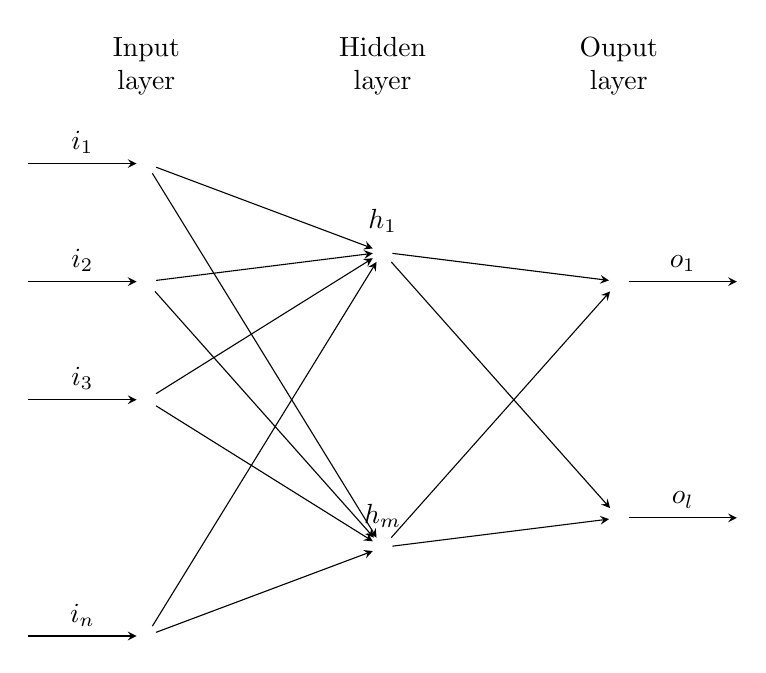
\begin{tikzpicture}[x=1.5cm, y=1.5cm, >=stealth]
	
	\foreach \m/\l [count=\y] in {1,2,3,missing,4}
	\node [every neuron/.try, neuron \m/.try] (input-\m) at (0,2.5-\y) {};
	
	\foreach \m [count=\y] in {1,missing,2}
	\node [every neuron/.try, neuron \m/.try ] (hidden-\m) at (2,2-\y*1.25) {};
	
	\foreach \m [count=\y] in {1,missing,2}
	\node [every neuron/.try, neuron \m/.try ] (output-\m) at (4,1.5-\y) {};
	
	\foreach \l [count=\i] in {1,2,3,n}
	\draw [<-] (input-\i) -- ++(-1,0)
	node [above, midway] {$i_\l$};
	
	\foreach \l [count=\i] in {1,m}
	\node [above] at (hidden-\i.north) {$h_\l$};
	
	\foreach \l [count=\i] in {1,l}
	\draw [->] (output-\i) -- ++(1,0)
	node [above, midway] {$o_\l$};
	
	\foreach \i in {1,...,4}
	\foreach \j in {1,...,2}
	\draw [->] (input-\i) -- (hidden-\j);
	
	\foreach \i in {1,...,2}
	\foreach \j in {1,...,2}
	\draw [->] (hidden-\i) -- (output-\j);
	
	\foreach \l [count=\x from 0] in {Input, Hidden, Ouput}
	\node [align=center, above] at (\x*2,2) {\l \\ layer};
	
	\end{tikzpicture}
	\caption{An example representation of a deep neural network with one fully-connected hidden layer.}
	\label{fig:fullyconnected}
\end{figure}


The input layer receives as input a column vector of input-features $i$ of size $n \in \mathbb{N}$. Every value of the hidden-layer represented by a vector $h$ of size $m \in \mathbb{N}$ is the result of a transformation of the input values given by \vref{eq:non_linear_transformation} where $w_1$ is a matrix of size $m \times n$ and $b_1$ is a bias term of size $m$. $g$ is a non-linear parametric function called activation function, which represents the core of neural networks. Subsequently, the second and last transformation manipulates the hidden layer $h$ to produce the values of the output layer following \vref{eq:non_linear_transformation} using $w_2$ with size $o \times m$ and $b_2$ with size $o$.  

\subsubsection{Learning process}

The learning process aims to seek a set of parameters $\theta$ that results in the best possible function approximation for a specific objective. In supervised learning, the actual output $Y$ is available for each particular input $X$, and it is used to update the parameters. The learning process can be carried out iteratively according to the following steps.

\paragraph{Forward pass} The input $X$ is forwarded through the neural network and the output $Y_pred = f(X, \theta)$ is gathered.

\paragraph{Loss} The resulting predicted value $Y_{pred}$ is compared with the actual value $Y$ computing the loss function $L(\theta)$. There are a lot of loss functions available to satisfy the particular needs of specific learning tasks. The \textit{error} is the difference between the output of the neural network for a specific input data and the actual value: it is essential to calculate the loss function. One of the most exploited loss function is the \textit{Mean-Squared Error} (MSE) \cite{shalev2014understanding} shown in \vref{eq:backprop} which works with L2-distance.

\begin{equation}\label{eq:backprop}
\begin{aligned}
L(y, \hat{y}) = (y_\theta - y)^2 \\
J = \frac{1}{n}\sum_{i=1}^{n}L(y_i, f(x_i))
\end{aligned}
\end{equation}

\paragraph{Backpropagation}
The next step is the computation of the global gradient of the loss  function $\nabla L(\theta)$ which is carried out together with its backpropagation through the network. The backpropagation algorithm \cite{rumelhart1988learning} calculates the local gradient of loss for each neuron in the hidden layers. The concept underlying this procedure and shown in \vref{eq:chainrule} is the \textit{chain rule} \cite{lecun2015deep}, which computes derivatives of composed functions by multiplying local derivatives.

\begin{equation}\label{eq:chainrule}
\begin{gathered}
y = g(x), \;\;\; z = f(g(x)),  \;\;\;
\frac{\partial z}{\partial x} = \frac{\partial z}{\partial y} \frac{\partial y}{\partial x}
\end{gathered}
\end{equation}


Therefore, the chain rule is exploited to propagate the calculate global gradient loss $\frac{\partial L(\theta)}{\partial \theta}$ back through the network, in the opposite direction of the forward pass.
The procedure calculates the local derivatives during the forward pass, while estimates the local gradient of loss during backpropagation determining the multiplication between the local derivative and the local gradient of the loss of the connected neuron of the next layer: if the neuron has multiple connections neurons, the algorithms adds up all the gradients.

\paragraph{Update} In this final step consists in the update of the weights of all neurons. There are many ways developed through the years to carry out the update phase, but the most common one is the gradient descent.
The objective of the gradient descent is to minimise the loss function by refreshing the internal parameters of the network in the negative direction of the gradient loss: this choice leads the function approximation process closer to the minimum at each iteration. \Vref{eq:update} describes the update rule presented by the gradient descent where $\alpha$ is the learning rate. The last-mentioned parameter determines how quickly the algorithm should approach the minimum. A higher learning rate leads to a greater step towards the minimum, which threatens to overshoot the target.

\begin{equation}\label{eq:update}
\theta \leftarrow \theta -\alpha \nabla_\theta J
\end{equation}

Nowadays, the techniques applied in the majority of research projects is stochastic gradient descent which combines batch learning \cite{stanford2019cs231n} and gradient descent, but also its various improved extensions and variants, such as ADAM \cite{kingma2014adam} and AdaGrad \cite{duchi2011adaptive}: these extensions manage to improve the convergence of SGD thanks to the introduction of adaptive learning rates.

\subsubsection{Regularization}

The final aim of the learning process is to obtain a function approximator capable of generalising over data. This fact means that a neural network should show performances on unseen data comparable to the one obtained from training data. For this reason, it is necessary an appropriate trade-off between underfitting and overfitting.

A shallow approximated function and insufficient training data with a lack of diversity are the leading cause to the first situation: the network generalises on the data, but the prediction error is always too high for all data points.
The phenomenon of overfitting describes the exact contrary of underfitting. The leading cause is too complex approximation function: this lead to a network which scores an excellent performance on training data, but poorly predicts unseen points.

Regularisation \cite{bishop2006pattern,lecun2015deep} represents an approach to overcome and prevent the problem of overfitting. It works extending the loss function with a regularised term $\Omega(\theta)$ as shown in \vref{eq:generalreg} where $\lambda$ is the regularisation factor. 

\begin{equation}\label{eq:generalreg}
L'(\theta) = L(\theta, Y, Y_{pred}) + \lambda \Omega(\theta)
\end{equation}

\Vref{eq:l2reg,eq:l1reg} show two examples of regularisation terms. The first is $L^2$-regularisation which exploits the squared sum of the weights $\theta$ in order to keep the weights small. The second approach is known as $L^1$-regularisation: in this case, large weights are less penalised, but this method leads to a sparser solution.
\begin{equation}\label{eq:l2reg}
L'(\theta) = L(\theta, Y, Y_{pred}) + \lambda \frac{1}{2}||\theta||^2 
\end{equation}
\begin{equation}\label{eq:l1reg}
L'(\theta) = L(\theta, Y, Y_{pred}) + \lambda \frac{1}{2}||\theta|| 
\end{equation}


\subsubsection{Activation function}

\todomacaluso{RESTART FROM HERE}

\Vref{eq:activation} shows the most common activation functions: in general, \textit{ReLu}  achieves better performance over a wide variety of tasks, but usually the selection of the best activation function has to be done starting from all information and requirements of the deep learning model.
\begin{equation}\label{eq:activation}
\begin{aligned}
\text{Sigmoid} \;\rightarrow\;& g(x) = \frac{1}{1+ e^{-x}}\\
\text{Hyperbolic Tangent} \;\rightarrow\;& g(x) = \frac{e^x-e^{-x}}{e^x+e^{-x}}\\
\text{Rectified Linear Unit (ReLu)} \;\rightarrow\;& g(x) = \max(0,x)
\end{aligned}
\end{equation}

\subsubsection{Batch Learning and Normalization}

\subsubsection{Convolutional Neural Networks}
Another crucial step in deep learning was the introduction of convolutional layers \cite{lecun1995convolutional}. This type of layer revealed is power with images, leading to an increasing interest in image processing field. The parameters of this layer are a set of filters (or kernels) with dimensions smaller than the whole input image: these filters are used to implement a convolution operation over the whole image, and the result serves the input to the next layer in the network. In this context, the network can learn filters that detect specific features in the image such as edges, textures and patterns \cite{erhan2009visualizing}.

\paragraph{Convolutional Layer}

\paragraph{Pooling Layer}


\subsection{Value-based methods}

The first class of algorithms to explore is the one of value-based methods. They works learning an approximator $Q_\theta(s,a)$ to infer the optimal action-value function $Q^*(s,a)$ using an objective function based on Bellman equations.
The preponderance of optimisations belonging to this category is \textit{off-policy}: this means that the optimisation step is done using all data collected during the whole training, not only with the most recent policy available. In this configuration, the information used for the learning phase could also come from exploration decision, apart from ones obtained with the most recent policy. 
Indeed, value-based approaches are more sample efficient because they can reuse data more efficiently, but they are considered less stable than policy gradient ones.
Thanks to the relation expressed by $a(s) = \operatornamewithlimits{argmax}_a Q_\theta(s,a)$, it is possible to obtain the policy learned so far from the current action-value function.

\subsubsection{Deep Q-Network (DQN)}
This algorithm grows from the ideas underlying Q-Learning \cite{watkins1989learning}  shown previously in \vref{tdlearn}. The team of DeepMind introduced the Deep Q-Network (DQN) in \cite{mnih2013playing} and in the next cutting-edge paper \cite{mnih2015human}: they managed to create an algorithm capable of learning to play ATARI video-games online using raw image and pixels. It works with neural networks as a function approximator, employing convolutional layers in the first layers of the neural network and performing the optimisation with a variant of stochastic gradient descent called RMSprop \cite{tieleman2012lecture}. The exploited neural network provides as output a probability distribution over all possible discrete actions to determine what is the best action to take.

To overcome the instability problem of value-based methods, DQN utilises two heuristics to narrow instabilities.

\paragraph{Target Network}
The presence of a second network, called \textit{target network}, enriches the update phase of this algorithm. \Vref{eq:lossdqn}
defines the loss function of DQN where $y_i$ value is computed using the target network instead of the local network. Therefore, the parameters of the target network are hard updated every $I \in \mathbb{N}$ iterations: this choice precludes instabilities and avoids divergence because of target networks parameters remain fixed for $I$ iterations.

\begin{equation} \label{eq:lossdqn}
\begin{gathered}
L_i(\theta_i)) = \mathbb{E}_{s, a \sim \pi}\big[(y_i - Q(s, a; \theta_i))^2\big]\\
y_i = \mathbb{E}_{s' \sim E}[r + \gamma \max_{a'}Q(s',a'; \theta_{i-1})|s,a]
\end{gathered}
\end{equation}

\paragraph{Experience Memory Replay}

Another crucial introduction in this algorithm is \textit{experience memory replay buffer} \cite{lin1992self}. Trajectories sampled from the environment are temporally correlated, and this could lead to over-fitting the parameters of the neural network. The setting of this algorithm is \textit{online} because the replay buffer stores $N_{\text{replay}} \in \mathbb{N}$ replacing old steps as new ones arrive. The experience is collected as tuples $<s_t,a_t,r_t,s_{t+1}>$ using the $\epsilon$-greedy policy. The learning phase samples a set of limited tuples called \textit{mini-batch} allowing a wider set of state-action pair in the update of the network and improving the procedure in terms of variance in respect of single tuple update.
Trajectories sampled from the environment are temporally correlated, and this could lead to over-fitting the parameters of the neural network. Using a batch sample from the replay buffer makes the data \textit{i.i.d.} and consequently improves the learning.

\subsubsection{Improvements of DQN}
Further investigation and speculation followed the publication of the thriving DQN. Summing up and comparing these new approaches to original DQN is the main aim of \textit{Rainbow} \cite{hessel2018rainbow}: it also introduces an algorithm called \textit{Rainbow DQN} with all the techniques proposed. The following paragraphs will delineate three main improvements of DQN.

\paragraph{Double DQN}
The Double DQN \cite{hasselt2010double, van2016deep} can handle the intricacy of overestimation of Q-values caused by the maximisation step in \vref{eq:lossdqn}. It works with two separate Q-Network with parameters $\theta$ and $\theta^-$ for estimating TD-target. It allows for removing the positive bias in estimating action values, leading to less overestimation of Q-learning values, improved stability and performance. In this context, the target $y_i$ is replaced by \vref{eq:ddqny}
\begin{equation} \label{eq:ddqny}
y_i = \mathbb{E}_{s' \sim E}[r + \gamma Q(s',\operatornamewithlimits{argmax}_aQ(s', a; \theta_{i-1}); \theta^-_{i-1})|s,a]
\end{equation}

\paragraph{Prioritized Experience Replay}

The fundamental idea underlying \textit{prioritized experience replay} \cite{schaul2015prioritized} is exactly to prioritise experiences that contain more crucial information than other ones. An additional value that defines the priority of a specific transition joins each tuple stored in the replay buffer: thanks to this approach, experiences with higher priority has a higher sampling probability and are more likely to remain longer in the replay buffer. It is possible to use \textit{TD-error} to measure the importance of each tuple in the experience. A high TD-error means that the agent behaved better or worse than expected in that particular moment, and therefore, it can learn more from that specific passage.

\paragraph{Dueling DQN}

The Dueling DQN architecture \cite{wang2015dueling} shown in \vref{fig:duelingdqn} works decoupling the Q-value estimation in two distinct sequences of fully-connected layers right after convolutional layers. These streams are capable of providing separate estimates of the state-value  $V(s; \theta, \beta)$ and advantage $A(s,a; \theta, \alpha)$ functions exploited in the end to obtain the Q-value function $Q(s,a; \theta, \alpha, \beta)$ estimate where $\theta$ represents the parameters of convolutional layers while $\alpha$ and $\beta$ the ones of state-value and advantage function respectively.

The first formalisation of the Q-value function is shown by \vref{eq:qvalueddqn0}, but \cite{wang2015dueling} also suggests a different approach \vref{eq:qvalueddqn1} which shown increased stability in practice.

\begin{gather} 
Q(s,a; \theta, \alpha, \beta) = V(s;\theta, \beta) + \big(A(s,a;\theta, \alpha) - \max_{a' \in \mathcal{A}}A(s, a'; \theta, \alpha)\big) \label{eq:qvalueddqn0}\\
Q(s,a; \theta, \alpha, \beta) = V(s;\theta, \beta) + \big(A(s,a;\theta, \alpha) - \frac{1}{|\mathcal{A}|}\sum_{a' \in \mathcal{A}}A(s, a'; \theta, \alpha)\big) \label{eq:qvalueddqn1}
\end{gather}


\begin{figure}
	\centering
	\begin{tikzpicture}
	 \node at (0,0) (image) {\includegraphics[width=0.7\textwidth]{img/duelingdqnn.png}};
	% node a_t
	\node[mylabel, below right=-0.1cm and -0.5cm of image.north] (action) {\LARGE \textcolor{Blue}{$\beta$}};
	\node[mylabel, above right=0.3cm and -0.5cm of image.south] (action) {\LARGE \textcolor{OliveGreen}{$\alpha$}};
	\node[mylabel, above right=0.8cm and -4.6cm of image.south] (action) {\LARGE \textcolor{PineGreen}{$\theta$}};% node s_t
	\end{tikzpicture}
	\caption[Dueling DQN]{\small Dueling DQN architecture \cite{wang2015dueling} representation taken from \cite{franccois2018introduction}. It consists in two stream to estimate state-value parametrized with $\beta$ and advantages values parametrized with $\alpha$ for each action. The last layer represent the combination of these two types of values. }
	\label{fig:duelingdqn}
\end{figure}


\subsection{Policy gradient methods}

Policy gradient algorithms aim to optimize the policy's performance measure in \vref{eq:pgperf} by finding a good policy $\pi_\theta(s|a)$ capable of generation a trajectory $\tau$ that maximizes the expected rewards \vref{eq:pgmax} instead of learning a  value function. Indeed the objective function in policy gradient methods consists of maximising $J(\theta)$ value by finding a good policy updating $\theta$ parameters directly.

\begin{gather} 
J(\theta) = \mathbb{E}\big[\sum_{t=0}^{N}r(s_t,a_t); \pi_\theta\big] = \sum_{\tau}P(\tau;\theta)r(\tau) \label{eq:pgperf}\\
\theta^* = \operatornamewithlimits{argmax}_\theta J(\theta) \label{eq:pgmax}
\end{gather}


The parameters of the policy $\theta$ are refreshed via stochastic gradient ascent. Gradient ascent is the inverse of gradient descent and updates the parameters $\theta_t$ in the positive direction of the gradient of the policy’s performance measure $\nabla_\theta J(\theta)$ following \vref{eq:pgascent} where $\alpha$ is the learning rate which defines the strength of the steps in the direction of the gradient.

\begin{equation} 
\theta_{t+1} \leftarrow \theta_t + \alpha \nabla_\theta J(\theta_t) \label{eq:pgascent}
\end{equation}

The main advantage of policy gradient approaches consists in the stability of their convergence: these methods work updating their policy directly at each time step instead of renewing value function from which to derive the policy like value-based methods. Last-mentioned approaches can lead to a radical change in the policy output even for a small change in the value function: this event can cause big oscillation during training.
Furthermore, policy gradient algorithms can face infinite and continuous action space because the agent estimates the action directly instead of calculating the Q-value for each possible discrete action.
The third feature is their ability to learn stochastic policies, useful in uncertain contexts or partially observable environments. 
Despite the presence of the advantages just mentioned, policy gradient methods have an important disadvantage: they rather converge to a local maximum than to the global optimum.

\subsubsection{Actor-Critic Architecture}

Actor-critic architecture, shown in \vref{fig:actorcritic} represents the point of contact between value-based approaches and policy gradient methods. They are policy gradient methods basically but exploit value-function to learn the parameters $\theta$ of the policy. As its name suggests, these approaches work with two different parts called \textit{actor} and \textit{critic} \cite{konda2000actor}. The \textit{actor} relates to the policy, while the \textit{critic} deals with the estimation of a value function (e.g.\ Q-value function). In the context of deep reinforcement learning, they can be represented using neural networks function approximator \cite{mnih2016asynchronous}: the actor exploits gradients derived from the policy gradient theorem and adjusts the policy parameters, while the critic estimates the approximate value function for the current policy $\pi$.

Standard practice is to update both networks with the \textit{TD-Error}, discussed in \vref{tdlearn}. Estimation made by the critic is useful to determine the contribution that expected values of the current and next state gives to the TD-error. Essentially, the output of the critic contributes to the update of the actor.

\begin{figure}[!h]
	\centering
	\includegraphics[width=0.5\textwidth]{img/actorcritic.png}
	\caption{\small Actor-critic architecture schema: the actor represents the policy and maps the input state to an output action, while the critic represents the value function. Both networks can be updated with, e.g.  the TD-error, using the contribution of the critic. It is noticeable that the actor uses the critic during the learning process \cite{sutton2018reinforcement}.}
	\label{fig:actorcritic}
\end{figure}

\subsection{Deep Deterministic Policy Gradient (DDPG)}

\subsection{Soft-Actor Critic (SAC)}

\section{Related Work}

\todomacaluso{
	\begin{itemize}
		\item Explanation of the state-of-the-art focusing more on Reda's paper, its approach and the related bibliography
\item Increasing interest in Reinforcement Learning applied to real-world situations, in contrast with simulated environments experiments
	\end{itemize}	
}

\section{Summary}








	\chapter{Tools and Frameworks} \label{ch:ch3}

This chapter aims to describe the main tools and frameworks used to develop the project of this thesis.
The first section will describe the OpenAI Gym framework, a central toolkit for developing and comparing reinforcement learning algorithms, and explain why this tool is essential for reinforcement learning research.
The second part of this chapter will outline Cozmo, the powerful toy robot developed by Anki that we used as an agent in the reinforcement learning scenario to apply algorithms to try solving autonomous self-driving tasks: \vref{ch:ch5} will report the analysis and description of these experiments.
This section will also report a set of available alternatives to Cozmo, explaining the motivations underlying the final choice.
The description about PyTorch, an optimised tensor library for deep learning using GPUs and CPUs used to build up the convolutional neural network of this work, and the related comparison with TensorFlow will occupy the last part of this chapter.

\section{OpenAI Gym}

Nowadays, OpenAI Gym \cite{brockman2016openai}, released in 2016 with its public beta, is one of the most popular toolkits and frameworks in the reinforcement learning scenario.
A brief analysis of reinforcement learning research could be useful to outline the motivations underlying the need for a reinforcement learning framework.

As reported previously in  \vref{ch:ch2}, reinforcement learning is a subfield of machine learning dedicated to the world of decision making and motor control: researchers study how an agent can learn and improve to achieve a specific goal in a complex, usually unknown environment.
This machine learning paradigm is becoming more and more attractive for both researchers and industries because of its visionary property of being very general.
A reinforcement learning algorithm can be exploited to control a robot's motor in order to make it capable of running or jumping, play a videogame or a board game, make critical business decisions like pricing and inventory management, but also learn how to invest in financial trading environments.
The generality of reinforcement learning became engaging thanks to the remarkable results achieved in many challenging environments, as reported previously in \vref{ch:ch2}.

Despite these appealing features, the research was slowed down by other circumstances, no less critical.
The need for better benchmarks represents the first factor.
As an example, the abundant availability of conspicuous datasets like \textit{ImageNet} \cite{deng2009imagenet} has driven supervised learning improvement in the research.
For what concerns reinforcement learning, the nearest equivalent to supervised learning datasets would be a broad collection of different environments in order to test various algorithms with different kinds of observations or rewards.
The second withdraw of this approach to learning is the lack of standardisation of environments designed in publications.
In reinforcement learning, subtle differences in problem definition, reward function design or action space typology could make the difficulty of the task grow.
This fact threatens to slow down and corrupts experiments reproducibility making an objective comparison between the results of different papers almost impossible.

The need to fix both problems was the primary motivation behind the design and implementation of OpenAI Gym.

\subsection{Environments}

The agent and the environment represent the main components of reinforcement learning.
The choice of OpenAI was to implement and provide the abstraction mainly for environments, not for agents.
They decide to provide a standard environment interface instead of forcing the developer to use pre-defined agent interfaces: the motivation behind this choice was to leave developers independent in the design of the agent, the core of reinforcement learning, and facilitate the creation and usage of environments.
Thanks to this approach, all agents implemented with OpenAI Gym can be used with the whole set of environments provided by the framework.
Therefore, it is possible to create a personalised environment to suit the needs of a specific experiment that can be used by all agents exploiting OpenAI Gym environment interfaces.

In this scenario, we realised the first contribution to our thesis.
Thanks to this framework features, we implemented an OpenAI Gym environment capable of interacting with Anki Cozmo by providing a binding between functions of Cozmo SDK and interfaces of the reinforcement learning framework.
In \vref{ch:ch4} we will provide further information and details about our contribution.

The importance related to the high quantity of environment is fundamental to build a reliable and sustainable framework for reinforcement learning algorithms.
For this reason, OpenAI Gym contains a various and heterogeneous environment database, ready to be used.

\subsubsection{Interface functions}

Exploring OpenAI Gym, it is essential to focus on the most crucial interface functions that the agent will exploit to interact with the environment.
The functions which constitute the skeleton of an OpenAI Gym environment are the following:
\begin{itemize}
	\item \texttt{def step(self, action)}: through this function, the agent can communicate the action it wants to take.
The input data depends on the type and number of variables in the actions space (e.g.\ discrete or continuous).
As will be discussed in \vref{subsec:observations}, the values returned by this function represent the environment state after the manipulation caused by the agent action.
Thanks to these data, the agent will be able to select the next action following the reinforcement learning loop.
	\item \texttt{def reset(self)}: during the episode, internal variables of the environment changes, influenced by the action taken previously.
This function allows the agent to restart the initial situation of the environment.
This procedure is particularly helpful when an episode finishes and the agent has to restart the next learning episode in a brand new copy of the environment.
	\item \texttt{def render(self, mode='human', close=False)}: this function is mainly used in simulated environments.
It enables the visual render (if available) of the environment.
	\item \texttt{def close(self)}: the final function to close the environment after the end of all experiments and episodes.
\end{itemize}

\subsubsection{Available environments}

To date, OpenAI Gym includes the following environments:
\begin{itemize}
	\item \textbf{Algorithms}: learning to imitate computations, such as copying or reversing symbols from the input tape, is the main aim of this typology.
These environments might seem easy to be solved by a computer, but it is essential to remember that the objective here is to learn to solve these tasks purely from examples.
Therefore, it is possible to vary the sequence length to increase or decrease task difficulties quickly.
	\item \textbf{Atari}: \textit{Atari 2600} is a home video game console developed in 1977 which spread the use of general-purpose CPUs into gaming with game code distributed through cartridges.
This environment section provides a database which contains more than 100 environments emulating Atari 2600 videogames.
OpenAI Gym exploits \textit{Arcade Learning Environment (ALE)} \cite{bellemare2013arcade} providing RAW pixel images or RAM as observation of the environment.
	\item \textbf{Box2D}: in this group is possible to find some continuous control tasks in a simple 2D simulator such as \textit{BipedalWalker}, \textit{CarRacing} and \textit{LunarLander}
	\item \textbf{Classic Control}: this class provides a set of problem borrowed by control theory and widely exploited in the classic reinforcement learning literature.
Some task examples are balancing a pole on a cart or swing up a pendulum.
	\item \textbf{MuJoCo}: this collection contains continuous control tasks running in a fast physics three-dimensional simulator called \textit{MuJoCo} which stands for \textit{Multi-Joint dynamics with Contact}.
This physics engine aims to facilitate research and development in robotics, biomechanics, graphics and animation.
The simulator is particularly suitable for model-based optimisation allowing to scale up computationally-intensive techniques.
	      Thanks to its features, it became useful as a source for reinforcement learning algorithms.
\cite{todorov2012mujoco}
	\item \textbf{Robotics}: OpenAI released this algorithm typology to provide eight robotics environments with manipulation tasks significantly more complicated than the MoJoCo ones.
It contains \textit{Fetch}, a robotic arm to move and grab objects, and \textit{ShadowHand}, a robotic hand to manipulate and grab pens, cubes and balls.
\cite{ingredientsRoboticsResearch}
\end{itemize}

\subsection{Observations} \label{subsec:observations}

As previously reported, the \texttt{step(self, action)} environment interface is the most important one because it contains the behaviour definition of the environment that reacts to agent actions.
Indeed, the agent has to know in which way its actions are influencing the environment in order to stop doing random actions and start making valuable decisions.

In order to provide this type of information to the agents, the \texttt{step} function returns four relevant values that reinforcement learning algorithms can exploit to determine the best action to do in the future.
These values are:
\begin{itemize}
	\item \textbf{\texttt{observation (object)}}: a specific object which represents the environment observation and shows the changes provoked by agent actions.
Its structure and interpretation depend on the implementation of the specific environment.
For example, it could represent the raw pixel data from a camera, the status of a board game or physics data of a robot (joint angles and velocities).
	\item \textbf{\texttt{reward (float)}}: this is the fuel of the reinforcement learning algorithms.
This value represents the reward achieved thanks to the action taken by the agent.
The reward for each action can change among environments, but this is the crucial information to enable the agent to learn.
	\item \textbf{\texttt{done (boolean)}}: this value is a simple boolean that signals the agent when the episode ended and it is time to reset the environment to start a brand new episode.
	\item \textbf{\texttt{info (dict)}}: a Python dictionary to monitor and show diagnostic information useful for debugging.
The agent could use it as additional information in the learning process, but the documentation of OpenAI Gym does not recommend to use this data in the learning process to maintain the coherence with the reinforcement learning loop.
\end{itemize}

The last important thing to report about the OpenAI Gym framework is the definition of \texttt{Spaces}.
As reported in the second chapter, an environment consists of the action space and the observation space.
Both can provide discrete or continuous values: this distinction is fundamental to determine the usage of a specific algorithm rather than others to solve a given task better.
For this reason, OpenAI Gym provides \texttt{Discrete} and \texttt{Box} to initialise discrete and continuous spaces, respectively.
It allows the user to define a lot of features useful in the learning process, such as a maximum and minimum value setup or a default function to sample a random value from the defined space instantly.

\section{Anki Cozmo}

\begin{figure}

	\begin{minipage}[t]{0.48\linewidth}
		\centering
		\includegraphics[height=0.25\paperwidth]{img/cozmo_inside_1.png}
	\end{minipage}
	\begin{minipage}[t]{0.48\linewidth}
		\centering
		\includegraphics[height=0.25\paperwidth]{img/cozmo_inside_2.png}
	\end{minipage}

	\caption[Anki Cozmo Robot]{On the left there is a photo of Anki Cozmo in action, while on the right side there is a graphical reconstruction of the whole set of gears and hardware inside the robot.}
	\label{fig:cozmo_inside}
\end{figure}

Especially in the latest decades, human beings have started a complicated relationship with robots.
They are very fascinated by the prospect of artificial intelligence offered by recent researches and applications.
However, they are apprehensive and worried at the same time because of the apocalyptic plot that many sci-fi films show and the significant promise of automation, capable of replacing human workers in the future.
However, all these concerns disappear after meeting Cozmo, the palm-sized toy robot developed by the San Francisco-based company Anki and available on the market since 2016.
On first glance, Cozmo might appear as one of the cutest toy robots: not surprisingly Anki employed the guidance of Carlos Baena, the former Pixar animator, to design this robot.
Therefore, it can interact with people using a small display screen together with audio effects to mimic human emotional reactions and responses.
The result is a toy robot WALL-E-inspired both aesthetically and personality-wise, powered up by artificial intelligence to move and discover the surrounding environment.
Thanks to the built-in camera, Cozmo can remember faces and recite names, but also to plan paths and play various games with its three cubes that carry sensors and lighting.

Despite these entertaining, but not so technical facts, Cozmo hides a lot of powerful features under the hood.
Anki developers produced a high-quality Python SDK that allows developers to take control of the whole set of Cozmo sensors and actuators thanks to the interaction granularity offered by functions and interfaces.
This section aims to outline the hardware and software architecture hidden underneath the cute Cozmo bodyworks, together with a comparison with the alternatives available to design the reinforcement learning system of this thesis.
An essential inspiration in the writing of this section came from \cite{mellon2017cognitive}, \cite{touretzky2018cozmopedia} and Anki Forums \footnote{Anki Cozmo SDK Forums: \href{https://forums.anki.com/}{https://forums.anki.com/}}.

\subsection{Cozmo architecture}

It is possible to define Cozmo as a vision-guided mobile manipulator, one of the first consumer robot which can boast vision among its features.
However, as reported before, the features it shows during the normal toy usage, do not equal the number of interfaces and functions made available to developers.
The hardware and the software developed for Cozmo makes it the right choice to fast prototyping computer science projects: it is the main reason why we decided to exploit Anki Cozmo instead of other alternatives.
The SDK provided by Anki consists of a comprehensive set of low- and high-level functions which grants full access to sensor data providing the right flexibility, simplicity and granularity to satisfy every developer needs.
It is versatile because it could be easily connected with hundreds of third-party libraries to augment Cozmo capabilities.
Therefore, it is an entirely open-source SDK to give the community the freedom to customise and contribute.

\Vref{fig:cozmotear1,fig:cozmotear2} shows technologies, the hardware and software involved in the production of Cozmo.
The first image represents stacks and connections between the robot core and the mobile application provided by Anki, while the second one shows the interaction between the last-mentioned application and the Python user program on the development machine.
The reader can retrieve a global perspective about the whole Cozmo architecture by merging these two figures.

\begin{figure}
	\centering
	\includegraphics[width=\textwidth]{img/cozmo-hw.png}
	\caption[Interaction Robot / Mobile Application]{Interaction between the Robot and the mobile application stack.
The main program of the robot interacts with the Cozmo Engine (C++) implemented in the mobile application through a proprietary TCP protocol established using an ad-hoc WiFi connection.
\cite{mellon2017cognitive}}
	\label{fig:cozmotear1}
\end{figure}

Analysing \vref{fig:cozmotear1}, it is noticeable that Cozmo has a lot of sensors and actuators, which enable it to move and understand the surrounding environment.
For what concerns the sensor part, the VGA Camera is the crucial component exploited in the thesis.
This camera provides a grayscale image with 320$\times$240.
Anki reported a camera resolution equal to 640$\times$480, but the latest firmware version supports only the lower resolution.
Furthermore, the camera can detect and acquire colours, but the firmware limits this feature to maintain the bandwidth stable and avoid overloads or slowdowns in the communication with the mobile application and subsequently, the user program running on the computer.
The camera has approximately 60° field of view (FOV) and 290mm focal length.

As regards the actuators column, Cozmo can explore the world thanks to its four motors and over fifty gears.
Instead of having wheels, this robot has two tracks to navigate: it can steer and move freely by controlling the speed of each track.
Another moving part is the head that can move up or down to direct the camera and the display.
It also has a forklift with which it can lift objects or the cubes available in the kit.

Cozmo can perform one single action at a time: if the current action is not yet complete and the request of a new action occurs, the new action fails with a \textit{tracks locked} failure code.
For this reason, the SDK does not allow the execution of multiple actions.
Despite this fact, it is easy to notice that Cozmo animations and behaviours typically use combinations of actions: indeed the user can send simultaneous actions to the robot by calling them using \texttt{in\_parallel=True} in its script, but these actions have to belong to a different action track.
This approach allows the parallel execution of actions, provided that they use different tracks.
Cozmo software architecture holds seven independent action tracks:

\begin{itemize}
	\item \textbf{HEAD}: raise/lower robot head.
	\item \textbf{LIFT}: raise/lower robot forklift.
	\item \textbf{BODY}: wheels or treads actions for driving and turning.
	\item \textbf{FACE\_IMAGE}: actions with the OLED display such as animations or faces.
	\item \textbf{EVENT}: for this action type Anki does not release further information.
	\item \textbf{BACKPACK\_LIGHTS}: actions or animations of lights on Cozmo back.
	\item \textbf{AUDIO}: speech or sound effects emitted by the robot.
\end{itemize}

The project of this thesis mainly exploited the body action track to move the robot in the environment: it also employed head and lift tracks, but only to position the robot head to provide images about the track to the main program and the reinforcement learning agent.
The usage of parallel operations was not necessary.

The Cozmo hardware includes an on-board CPU and a WiFi access point, thanks to which the user can interact with the robot.
However, to activate this communication, it is necessary to install the Cozmo Android/iOS application on a personal tablet or smartphone.
This application is the same used to play with the toy-side of Cozmo, but in its settings, there is a function to enable Cozmo development mode.
After connecting the chosen personal device to the robot through a simple WiFi connection, the application manages to create a proprietary TCP protocol to interact directly with the main robot program.
The creators of Cozmo developed this mobile application using C++ to implement the \textit{Cozmo Engine}, the component which shall be responsible for the TCP communication with the robot.
To design and implement the game experience and the graphical user interface, they used Unity and C\#.

This last-mentioned part utilises the component internally designed and implemented by Anki to provide a contact point between the Cozmo SDK installed in the development machine, as shown in \vref{fig:cozmotear2}: the C-like Abstract Data language (CLAD).
The fundamental idea behind this tool is to make the process of serialisation, communication and deserialisation of data structures written in Python easier for the developer.
In practice, for every data which has to pass over the wire, files with extension \texttt{.clad} to define enums, structures and messages are generated: their syntax is similar to C struct one.
After that phase, this tool auto-generates Python, C++ and C\# code for each structure previously defined.
This process allows the user to define a specific message in Python and to send it to the C++ engine where it will be deserialised automatically, avoiding problems and sources of bugs coming from intricate underlying details.

\begin{figure}
	\centering
	\includegraphics[width=\textwidth]{img/cozmo-sw.png}
	\caption[Interaction Mobile Application / Computer]{Interaction between the mobile application stack and the Python user program.
Anki designed a C-like Abstract Data Language (CLAD) to implement the connection between the Cozmo SDK and the Cozmo Engine on the mobile application.
This approach puts a decoupling layer between Python interfaces and low-level functions to make prototyping easier and fast-forwarding for developers.
\cite{mellon2017cognitive}}
	\label{fig:cozmotear2}
\end{figure}

This approach results in a process method much lighter than the one provided by \textit{Protocol Buffers (Protobuf)} by Google: even then, the main aim of this implementation choice was reducing the network bandwidth.
Taking all arguments into account, CLAD is the protocol used for the interaction between the SDK and the C++ Engine that allows the developer to not care about the low-level part of the code and to focus on the high-level logic using Python.
It is also useful to maintain the same interface for the user even if low-level logic changes occur.

In this case, the CLAD communication messages exploit a wired connection between the mobile device and the computer with a simple USB cable.
In this thesis, we used an Android tablet to run the experiments, and for this reason, we used the \textit{Android Debug Bridge (ADB)} to make this exchange possible.
It is a command-line tool included in the \textit{Android SDK Platform-Tools} package that allows the communication between the computer and Android devices.
It facilitates many device actions such as installing, debugging apps or running a variety of commands on a device.
It is a client-server program that consists of three components: it includes a \textit{client} hosted in the development machine, a \textit{daemon (adbd)} which runs the commands on the device as a background process and finally a \textit{server}, a background process in the development machine that manages the communication between the two previous components.

The last step to start programming with Cozmo SDK is to install it in a development machine following the instruction provided by its documentation \footnote{Cozmo SDK Documentation: \href{http://cozmosdk.anki.com/docs/index.html}{http://cozmosdk.anki.com/docs/}}.


\subsection{Why Cozmo?}

Before starting the development of this thesis project, we spent some time analysing the small car market situation in order to find out the right choice for our specific needs.
In addition to Anki Cozmo, the ideal alternatives in the self-driving scenario when we started this thesis were \textit{AWS DeepRacer Vehicle} and a customised vehicle implemented from scratch exploiting \textit{Donkey \textregistered
	Car library}.

This section part aims to briefly describe the main alternatives to Anki Cozmo listing strengths and weaknesses for each approach to motivate the final choice made.

\subsubsection{AWS DeepRacer}

\textit{AWS DeepRacer} is a platform developed by Amazon to learn and refine machine learning, reinforcement learning algorithms and techniques on AWS DeepRacer vehicle.

The whole ecosystem consists of two main part:
\begin{itemize}
	\item \textbf{AWS DeepRacer Car}.
It is a 1/18 scale race car developed and built to test reinforcement learning algorithms on a real track.
It aims to show how the reinforcement learning model trained in a simulated environment can be conveyed to the real-world by using cameras to view the track and the model to control throttle and steering.
It has a lot of impressive specifications under the hood such as Intel Atom \textsuperscript{\textregistered} Processor, 4GB of RAM, an expandable 32GB of storage to accommodate the trained model and a 4-megapixel camera with MJPEG.
	\item \textbf{AWS DeepRacer Simulator}.
The user can build his models in \textit{Amazon SageMaker} and train, test and iterate the learning process using the racing simulator.
It offers an integrated environment hosted on the AWS cloud to experiment and optimise algorithms to apply to the autonomous driving model.
\end{itemize}

There are many advantages in using the DeepRacer stack.
It offers an integrated approach where the developer has to focus just on reinforcement learning: indeed, it abstracts a significant part of the software giving the developer the chance to work almost exclusively on the model.
It has a growing development community to confront ideas and find solutions through challenging competitions around the world.
One of the fundamental aims behind this product is to build up a regulated environment where amateurs and researchers can compare and tests different approaches in solving the autonomous driving task.
Therefore it provides a high-performance car where to store the trained model in order to make it independent to the training environment.


On the other hand, one of the main disadvantages of this approach is that it is an Amazon lock-in: the framework provided force developer to use the whole Amazon stack.
This fact can be inconvenient economically-wise because of the rates of the Amazon platform that adds to the price of the car, but, above all, because Amazon may have access to all developer implementations and experiments.

Another not negligible factor was the product release date: Amazon had to release it in July, but, to date, it is not yet available in Italy.
Therefore, because of this thesis is focused on the application of reinforcement learning algorithms directly in the real world without the aid of simulators and model, the absence of the physical car was crucial for the final decision.

Another important withdraw consists of the strict correlation between the simulator and the real system: the framework provided by Amazon seems to be suitable only to test reinforcement learning algorithms after the model training in the simulator, but not for the sake of this thesis.

\subsubsection{Donkey\textregistered Car}

The second important alternative to Cozmo was to develop a small car from scratch using integrated boards such as \textit{RaspberryPi} or \textit{NVIDIA Jetson Nano}, sensors and camera to personalise the device and satisfy specific project needs.
\textit{Donkey\textregistered Car} \footnote{Donkey Car community website: \href{https://www.donkeycar.com}{https://www.donkeycar.com}} is the most popular choice to build a personal self driving toy car.
It is an open-source community project powered by volunteers who are interested in build their own self-driving cars.
They cooperated to build up a high-level self-driving library written in Python, focusing on enabling fast experimentation and contribution.
They provide detailed instructions to build a personal Donkey vehicle, providing kits or lists of components to use: the whole kit costs among 250-300\$.

It is also possible to install the Donkey library on any RC car to make it self-driving and autonomous.
Despite this fact, Donkey developers suggest building the \textit{Donkey2} car, which is a tested hardware and software setup, to avoid problems such as incompatibilities or bugs and make the most out of the presence of a dense community.

The main strength of this choice is the freedom to develop a completely customised car to suit better the needs and requirements of a great set of autonomous driving projects.
In the last releases of the library, Donkey developers released a complete sandbox simulator for training a self-driving car.
The languages used to develop it are Unity for simulation and Python with Keras and Tensorflow for training.
They also provide an OpenAI Gym environment to use with such simulator.

The main weakness of this method consists in the process of building a self-driving car system from scratch.
It offers versatility and flexibility in components choice, but the time to devote to building a working system, free from as many bugs as possible would have slowed down the prototyping of the system itself and the whole thesis project.
The duration of development is not associated with the process of physically assembling the car because Donkey developers estimate two hours to build the car.
The real obstacle consists of the setup of a connection similar to the Cozmo one: it needs to be as stable as possible to make all stack working smoothly in real-time.

\subsubsection{The final choice}

As easily predictable, the final choice fell on Anki Cozmo.
It provides a fast-forwarding SDK ready to be exploited in prototyping a brand new project together with the strictly necessary sensors to perform the reinforcement learning experiments in the real world.
A crucial factor in reaching the final decision was the dimension of the car: Donkey and Amazon DeepRacer are 1/10 and 1/18 scale race cars respectively, while Cozmo is just 5.5cm wide, which results in a ratio of about 1/30.
This fact not only makes Cozmo an easily transportable solution to speed up experiments and to restart episodes effortlessly but also a solution that supports the design of a track in a restrict space such as the one in the laboratory of Eurecom.

Therefore, the connection between the development machine and the robot is suitable for implementing an OpenAI Gym environment, and it is similar, at least in the premises, to the distributed off-board computation approach.
The main algorithm, the neural network, the reinforcement learning framework and the other cognitive parts are computed and managed by the workstation, instead of being stored in the vehicle as happens in Amazon DeepRacer and Donkey car approaches.

Taking into account the perspective of autonomous cars in the real world, on-board and off-board computation approaches are still under research.
With the on-board method, cars have much computational hardware inside in order to manage every aspect of autonomous driving by themselves, but it requires more powerful batteries to counterbalance energy consumption.
On the other hand, the connection to off-board computer facilities or the clouds leads to new vectors of attack but also enables companies to monitor the behaviour of the vehicle fleet to identify malicious activities early.
To date, both approaches are still under research, and it is not possible to decree a legitimate winner.
For what concerns the thesis, the designed system emulates an off-board approach.

In the end, Cozmo provides plain and straightforward control of the car, a rich Python SDK to use with OpenAI Gym, and it is the best trade-off between functionalities and fast-developing.

\section{PyTorch}

PyTorch \footnote{PyTorch Github Repository: \href{https://github.com/pytorch/pytorch}{https://github.com/pytorch/pytorch}} \cite{paszke2017automatic}  is an open-source machine learning and deep learning library developed by Facebook's AI Research Lab and released to the public in October 2016.
The main aim of PyTorch is to provide an intuitive and straightforward framework to develop artificial intelligence projects: two of the main applications to date are computer vision and natural language processing.

The programming languages utilised to develop PyTorch were Python, C++ and CUDA, the parallel computing and API model created by Nvidia to allow software developers and engineers to use CUDA-enabled GPU for general purpose processing.
The primary interface provided by the library to the user employs Python, the project where Facebook developers mainly put their efforts.
Despite this fact, it also offers a C++ interface.

PyTorch consists of the following components:
\begin{itemize}
	\item \textbf{\texttt{torch}}: PyTorch Tensor library with strong GPU support.
It implements interfaces similar to those of the NumPy library.
It contains data structures for multi-dimensional tensors and mathematical operations, providing many utilities for efficient serialising tensors and arbitrary types.
	\item \textbf{\texttt{torch.autograd}}: the tape-based automatic differentiation library that supports every differentiable operation on tensors available in \texttt{torch}.
	\item \textbf{\texttt{torch.jit}}: this component is a compilation stack that uses TorchScript to create serializable and optimizable models from PyTorch code.
This tool allows the user to train models in PyTorch using Python and then export the model in a production environment where Python may be disadvantageous for performance and multi-threading reasons.
	\item \textbf{\texttt{torch.nn}}: this component provides a neural networks library that is entirely compatible with \texttt{autograd} and designed for flexibility.
	\item \textbf{\texttt{torch.multiprocessing}}: this component is based on the Python multiprocessing library, but it implements memory sharing of torch tensors across processes.
	\item \textbf{\texttt{torch.utils}}: it contains many utility functions to better exploits the features of PyTorch.
\end{itemize}

PyTorch provides a NumPy-like experience to interact and manipulate data structures suitable for GPU computation, offering a deep learning research platform which can provide flexibility and speed.
These data structures are called \textit{Tensors} and they can be used both on the CPU and the GPU, accelerating the computation thanks to the whole set of functions and manipulators explicitly designed for every scientific computation need.

PyTorch is not a straightforward binding to an underlying complex C++ framework.
The library design focused on establishing Python as the main priority, and for this reason, the user experience is very natural and similar to other important machine learning libraries already present in the package manager.

It is noticeable that PyTorch developers aimed to create an intuitive and linear product to use.
To follow this idea, they decided to make PyTorch synchronous to permit the debugger to receive and understand messages and stack traces promptly.
This feature translates in a better debugging experience for the end-user.

Beyond these features, one of the traits that distinguish PyTorch from other frameworks is its single way to build neural networks by using a tape-based automatic differentiation.
The majority of deep learning frameworks available in the market, such as TensorFlow, Theano or Caffe, exploits a static approach in structure computation graph creation: they reuse the same layout in the whole program, therefore changing a simple component triggers the regeneration of the graph from scratch.
PyTorch utilises an entirely different approach which is not unique to PyTorch, but it provides one of the fastest implementations: they call it \textit{Tape-Based Autograd}.
This term refers to the reverse-mode automatic differentiation exploited in the framework, which is a technique based on the properties of the chain rule: to calculate the derivative of an output variable w.r.t. any intermediate or input variable, the only requirement is to know the derivatives of its parents and the formula to calculate derivative of primitive expression.
The main improvement that this approach brings is allowing the user to change the network structure on-the-fly without lag or overhead.

\subsection{TensorboardX}

One of the most crucial means that every machine learning researchers need is a tool to visualise and measure data efficiently: this fact is significant because we need to measure in order to improve models, projects and results.
However, one of the main problem in PyTorch is the absence of such a tool, specifically designed for the Facebook framework.
It can always use powerful tools such as \textit{Matplotlib}, but it offers a synchronous approach that leads to slow down the main program since the primary process has to wait for the data rendering before starting next operations.

On the other hand, TensorFlow, the most important deep learning alternative to PyTorch developed by Google, provides in its package TensorBoard which is a webserver to serve visualisation of the training progress of the neural network.
It can show to the user scalar values, images or text, and it is particularly useful to visualise experimental metrics such as loss and accuracy.
The particularity of this tool consists in the fact that it stores these typologies of information asynchronously as events.
The Python script calls specific functions to store information and goes on with the next operation without waiting for its render: that is possible thanks to the decoupling level inserted by this approach between the visualisation and the creation of data.
Indeed, Tensorboard operates by opening and reading  TensorFlow events files that contain the summary data generated during experiments.
Therefore, it will be the webserver to take care of elaborate data for rendering without bothering the current Python script.

Fortunately, PyTorch can exploit the features of Tensorboard thanks to a library called \textit{TensorboardX} \footnote{TensorBoardX documentation: \href{https://tensorboardx.readthedocs.io/en/latest/index.html}{https://tensorboardx.readthedocs.io/}} that stands for \textit{Tensorboard for X} to highlight developers aim to make Tensorboard available for all deep learning framework.

\subsection{Comparison with TensorFlow}

After the advent of deep learning, many companies decided to put their efforts to design architectures and frameworks to vehiculate this new technology.
The two most popular frameworks in this research field are TensorFlow \cite{abadi2016tensorflow} by Google released in 2015 and PyTorch \cite{paszke2017automatic}  by Facebook released in 2017.

Implementing the same neural network in these two frameworks will lead to different results because of the training process has many parameters that depend on the underlying technologies provided by the specific framework.
For instance, the training process in PyTorch is enhanced by CUDA GPU usage, while TensorFlow can access to GPU through its GPU acceleration.
The choice between these two frameworks is not straightforward because it depends on the perspective and the needs of the specific projects to develop.
For this reason, this section aims to outline differences between these two libraries without aiming to decree the best one but to motivate the decision we made using PyTorch.

\subsubsection{Dynamic versus Static}

The first difference concerns the construction of the computational graph.
A computational graph is an abstraction useful to represent the computation process through a direct graph.

In TensorFlow, computational graphs are defined statically, before running the code.
The main advantage of this method is allowing parallelism and dependency driving scheduling, features that boost the learning and make it more efficient.
This framework communicates with the external world via specific tensors that will be substituted by input data at runtime.
Only with TensorFlow 2.0, Google decided to implement dynamic computational graph in its product, but its stable version was released after the start of this thesis.

As mentioned above, PyTorch approach to computational graphs is dynamic.
This characteristic means that the graph is built incrementally at runtime without using particular data structures as placeholders.
This feature supports projects where the author needs to change the computational graph on-the-fly avoiding the application restart.
In this sense, PyTorch is more pythonic than TensorFlow \cite{builtin2019pytorch}.

\subsubsection{Distributed training}

Another key feature is the distributed training and data parallelism.
PyTorch offers native support for asynchronous execution from Python, and then it could improve performances.
On the other hand, TensorFlow needs more efforts to allow distributed training: the developer must fine-tune every computation to make it running on a specific device.
Both frameworks offer the same opportunities in these terms.
However, TensorFlow needs more effort to make things work.

\subsubsection{Visualisation}

As discussed in the previous section, TensorFlow exploits TensorBoard to provide all tools that machine learning researcher needs to visualise learning and keep track of the training process.
Facebook researchers developed \textit{Visdom} for this purpose, but it provides very minimalistic and limited features compared to the ones offered by TensorBoard.
As reported before, it is possible to use TensorBoard with PyTorch thanks to the library TensorBoardX.

\subsubsection{Production deployment}

For what concerns the deployment of trained models into production, TensorFlow offers the best service via \textit{TensorFlow serving}, a framework that offers and uses REST Client API.
The production deployment in PyTorch improved from its early releases, but, currently, it does not provide a framework to deploy the trained models on the web: the developers must use Flask or Django as backend server to provide the right environment to exploit the model.

\subsubsection{Conclusions}

Considering all the points explained in this section, we decided to utilise PyTorch for this project, but it is noticeable that there is no winner in this comparison.

Both frameworks have strengths and weaknesses that depends on the specific applications where we would use them.
TensorFlow is a mature and robust tool, notably suggested for production and AI-related products.
Although it needs some time to get the developer used to its programming approach and, at least at the start of this thesis project,  it supports only static computational graph methods.
On the other side, PyTorch is an efficient and young framework with a large community and which provides dynamic computational graphs and is more Python friendly.
Therefore, it is especially recommended for research-oriented developers.
	\chapter{Design of the control system}\label{ch:ch4}

In the previous chapters, we outlined deep reinforcement learning fundamentals with its most critical underlying concepts, and then we discussed the choice made about the technologies to use as baselines for our experiments.
The decision fell on Anki Cozmo because of the high-quality SDK provided to developers, its dimension and its features, while for what concerns the deep learning framework we opted for the versatility and flexibility provided by PyTorch, particularly suitable for a research context.

The following step in the path of this thesis consists of merging reinforcement learning theory with tools and frameworks presented previously to create the system in question.
Indeed, this chapter aims to describe the design of the control system for reinforcement learning experiments with Anki Cozmo.
The work presented in this part represents one of the contributions of our thesis and the necessary step towards reinforcement learning experiments.

The outline of the whole ecosystem with the description of interfaces, frameworks and technologies used occupies the first section of the chapter.
This part also comprehends the description about the implementation of the OpenAI Gym environment to make reinforcement learning algorithms interact with Cozmo, emphasising its differences from a typical simulated environment: we will start from the problem formalisation as Markov Decision Process (MDP) to conclude with the implementation of human-robot interaction.

We already presented the theory underlying DDPG~\cite{lillicrap2015continuous} and SAC~\cite{haarnoja2018soft, haarnoja2018alg} algorithms in \vref{ch:ch2}.
For this reason, the second section consists of a discussion about the specificities of reinforcement learning implementations we built with references to the choice we made in terms of hyper-parameters and neural network design in a real-world application.
In the final section of this chapter, we will present some relevant problem we faced in the design and setup of the real-world track together with the decision we made to overcome them.

\section{Outline of the system}\label{sec:outline-of-the-system}

% TODO: DDPG-SAC?
The development of the control system for Anki Cozmo was the main contribution of the thesis, together with the implementation of SAC algorithm.
The main aim of this work was to create an OpenAI Gym environment capable of interacting with a robot in the real world without any interaction, fine-tuning or prior knowledge obtained through the use of a simulator.
OpenAI Gym usually provides plain and straightforward interfaces to interact with simulated environments: we decided to exploit these functions to allow the application of reinforcement learning algorithm directly in the real-world decision of the robot.


The fundamental source of inspiration to develop this control system was~\cite{kendall2018learning,kendall2019learning}.
This publication represents, as its authors reported, the first reinforcement learning self-driving experiment where a car learned to drive through the application of a reinforcement learning algorithm, by trial and error.
They first trained the model exploiting Deep Deterministic Policy Gradient (DDPG) in a simulator for many epochs to find the most suitable hyper-parameters to use.
After this simulated learning process, they started their experiments in the real world using the set of parameters obtained from preceding experiments.
Unfortunately, the authors did not describe in details the fine-tuning process in the simulation and did not provide the results of these experiments in order to allow a weighted comparison with the real-world experiment.
They revealed only a  table with a report of the best performance for each model.
This fact, accompanied by the challenging prerogatives of this type of experimentation, was the propulsive thrust that led us to attempt to implement a similar reinforcement learning configuration without any prior help from simulations.

We decided to export and implement these ideas in our project, adapting them to the specificities and particularities of the Cozmo setup.
\Vref{fig:system} summarises the resulting system providing a schematic overview of every technology employed and interactions among them.
This section aims to describe as clearly as possible all the components of the control system we designed.

\tikzset{every picture/.style={line width=0.75pt}} %set default line width to 0.75pt        

\begin{figure}
    \centering
    \includegraphics[width=\textwidth]{img/cozmo-system.png}
    \caption[Outline of the control system]{The interaction between the user and Anki Cozmo has a crucial role in this system.
        The main Python script utilises OpenAI Gym for the reinforcement learning component and PyTorch for the deep learning one.
        The user can interact with the flow of the system through a simple web app that uses OpenAI Gym and the Cozmo SDK directly to provide information for the user (e.g.\ images, learning information) and the robot (e.g.\ commands).
        The last component consists of TensorBoard thanks to which the script can store results that can be retrieved later by the user.}
    \label{fig:system}
\end{figure}

\subsection{OpenAI Gym Cozmo Environment}

Before starting the description of the system we designed to carry out reinforcement learning experiments it is necessary to outline the decisions we made about what to implement in \textit{CozmoDriver}, the OpenAI Gym environment we developed to apply, train and test reinforcement learning algorithms with Cozmo.

The path of this section will follow the steps of a typical formalisation of the Markov Decision Process (MDP), bringing out the problems encountered, the reasoning behind them and solutions proposed as they go.

\subsubsection{Markov Decision Process Formalisation} \label{subsubsec:mdp_form}

Starting from the definition of MDP that we already reported in~\vref{eq:mdp}, we studied and investigated the best configuration to provide an acceptable trade-off between performance and memory consumption, capable of making the system work on the development machine we used for our experiments.
In the following paragraphs, we will analyse each MDP aspects paying particular attention to the problems we faced and the motivations behind every decision made to overcome them.

\paragraph{State/Observation Space}
The environment observation is the group of information that the reinforcement learning agent can see and obtain from the interaction with the real world.
Current autonomous driving technology usually works thanks to the presence of various sensor positioned in different points of the car body as we discussed in \vref{sec:related-work}.
However, this approach is quite different from what human beings use to guide every day: the only input that the human receives is what he sees.
Taking this fact into account, in the self-driving tasks in question, we thought that the most reasonable way to obtain knowledge about the surrounding environment as similar as possible to how humans do was to exploit front camera images provided by Cozmo SDK.
However, it is essential to remember that, by definition, the state must satisfy the Markov property.
According to this definition, \textit{the state must be independent of the past given the present}.
For this reason, using a single image to describe the current state may be an oversimplification of the problem.
Even a human would not be able to determine the best action to take starting from a single frame.
That is because it is difficult to infer or determine the current direction of the car, speed or steering wheel position.
Merely adding another image can intuitively improve the human perception of the scene: as an example, the first intuition this introduction could reveal is where the car is going, allowing the user to decide more accurately about the trajectory to follow.

To verify this fact before starting the experiments with the application of the reinforcement learning algorithms to Cozmo, we firstly analysed the results of some experiments on the environment of the classic control problem of trying to keep a frictionless pendulum standing up (\textit{Pendulum-v0}).
The original version of this environment utilises angle position and trigonometric results as observation to return to the agent.
However, this environment offers to the user the access to the images provided by the OpenAI Gym \texttt{render} interface.
It represents an entirely different kind of experiment from Cozmo driving task, but they have in common the improvement in trajectory inference brought by the presence of a number of pictures higher than one.
In order to make this environment suitable for convolutional neural networks, we decided to appropriately modify it to exploit raw images as observations instead of the original information.
Therefore, we noticed that the usage of a single picture as observation led to unstable and worse results than the ones obtained by combining two subsequential images to feed the algorithm.
For this reason, we decided to use two consecutive raw images provided by Cozmo by using a queue data structure with size two.
In the code flow, the developer merely has to push the next image obtained from the robot and use the specific queue function implemented to obtain the concatenation of the last two images, only when necessary.

Therefore, we decided to reduce the original size of the input Cozmo image to 64$\times$64.
We made this decision as a trade-off between performance, learning phase duration and space available in the central memory to store the replay memory.

In conclusion, the observation provided to the agent is the concatenation of two grayscale images with dimension 64$\times$64 pixels.

\paragraph{Action Space}

Another essential part that we needed to formalise is the action space, how the agent can interact and influence the surrounding environment.
In the car scenario, the two main components of driving are the speed of the vehicle and the position of the steering wheel.
To straightforwardly formalise these two parts, we decided to use two simple real values.

We chose to define the desired speed value in a range of 0 to 1, while we opted for a range of -1 to 1 for the steering wheel position.
These limits allow the agent to manipulate simple values in the decision-making process and to facilitate the manipulation of neural network results.
At the same time, the underlying logic of the environment takes care to translate these values into a compatible format for the Cozmo SDK.
Indeed, as reported in \vref{subsec:human-robot-interaction}, the Cozmo SDK function exploited to manoeuvre the robot needs at least the speed of each tread.
\Vref{conversionCozmoDriver} reports key steps of this translation.
Therefore we decided to raise acceleration parameters by setting them equal to 4 times the velocity of each thread to reach the desired speed as fast as possible.

\begin{algorithm}[!h]
    \SetAlgoLined
    \small
    \DontPrintSemicolon
    \LinesNumbered
    \KwIn{Desired speed $s_t \in \{ x \in \mathbb{R} | 0 \le x \le 1 \}$\newline Steering wheel position $w_t \in \{ x \in \mathbb{R} | -1 \le x \le 1\} $\newline Maximum forward speed $s^{\text{forward}}_{\text{max}} = 150\text{mm/s}$\newline Maximum turning speed $s^{\text{turning}}_{\text{max}} = 100\text{mm/s}$}

    Left tread speed: $ts_{\text{left}} = s_t \cdot s^{\text{forward}}_{\text{max}} + w_t \cdot s^{\text{turning}}_{\text{max}}$\;
    Right tread speed: $ts_{\text{right}} = s_t \cdot s^{\text{forward}}_{\text{max}} - w_t \cdot s^{\text{turning}}_{\text{max}}$

    \KwOut{Left tread speed $ts_{\text{left}}$ \newline Right tread speed: $ts_{\text{right}}$}
    \caption{CozmoDriver actions conversion from virtual to real}
    \label{conversionCozmoDriver}
\end{algorithm}


\paragraph{Reward Function}

The reward function is the crucial feature to define in the formalisation of the MDP.
After a review of the available literature and the analysis of the problem, we obtained a list of ideas and concepts to model the reward function:

\begin{itemize}
    \item \textbf{Lane Distance}: this model calculates the reward of each action by calculating the distance between the car and the centre of the lane.
          The main aim is to prioritise the correct positioning of the car on the lane, crucial for driving safety.
          However, it is noticeable that this value can be easily calculated in a simulated environment, while it needs a lot of sensors and calculations to obtain a good estimation in a real-world environment.
          Beyond this problem, this approach has difficulties in scaling to varying environments where road typology and dimension is not a pre-configured constant.
          Therefore, it is a limited approach because human beings do not always drive the car in the perfect centre of the lane: for instance, when approaching a curve, it could be more convenient to move the car slightly away from the perfect centre.

          This fact reveals the shortcomings of this approach: the system can perform only as good as the human intuition underlying the hand-crafted lane reward.

    \item \textbf{Distance Covered}: the second approach we investigated was the one suggested by~\cite{kendall2018learning,kendall2019learning}, where the reward of a specific action consists of the total distance covered by the car for each specific action taken.
          Approaching the problems with this method leads to results that can be easily understandable for humans: indeed, the total reward of each episode represents the total distance travelled by the robot.

          In the car scenario of the previously mentioned publication, it is possible to use the car odometry device to quickly retrieve this value after each action and calculate the reward of a specific decision obtaining the difference with the previous value.
          Cozmo does not have such kind of sensor on board.
          Therefore it is necessary to calculate this value manually.
          The intuition behind a reasonable estimation of the distance covered by Cozmo consists of using the fundamental formula of kinematics: the speed.
          Indeed, in the designed system, we have direct access to the aspired speed because it is a parameter that the agents decide at each iteration, and it is possible to derive the time elapsed between one action and its following one by manually calculating them inside the OpenAI Gym environment.

    \item \textbf{Speed Crash Penalty}: the third typology of reward we investigated consists of a sort of life bonus reward.
          The robot receives a reward (e.g.\ 1 point) for each timestep of correct decisions and a negative reward (e.g.\ -10 points) every time the user stops the robot preventing the crash.
          Therefore we added to the positive reward a small quantity that depends on the current speed to encourage the robot to stay on track and increase its speed.
          Consequently, we decided to add a penalty in faulty time step proportional to the robot crash speed to entice the robot in avoiding high speed when close to critical points.
          \Vref{eq:speedCrashPenalty} formalises the reward used in this approach: $p_1$ and $p_2$ are two parameters that determine how much the speed influence the reward and their module must be much less than the constant value in the equation to highlight the fact that they represent a secondary objective \cite{raffin2019learning}.
          \begin{equation}
              r_t = \begin{cases}
                  +1 + p_1 \cdot s_t, & \mbox{if } \mbox{Cozmo on the track} \\ -10 - p_2 \cdot s_t, & \mbox{if } \mbox{Cozmo off the track}
              \end{cases}
              \label{eq:speedCrashPenalty}
          \end{equation}

\end{itemize}

After the analysis of these three reward design proposal, we decided to select the second one to pursue our experiments in the real world.
As previously reported, the first option would have been hard to carry on and to scale up.
The third option hints intriguing facts that a reinforcement learning agent could take into account to better solve the driving task of our experiments.
The only withdrawal of this approach is related to the correlation between reward and distance covered: this correspondence is significant for the developer to have a more transparent overview of what is happening and how the algorithm is learning, at least in the early stages of development.
In the second option, the distance covered by the robot is equal to the reward, while this conformity is lacking in the third option.
For this reason, we decided to take the second reward proposal for this time.
We noticed that it could be an exciting future development trying to merge the second alternative with the third one to obtain a brand new reward function that both penalises bad decisions proportionally to speed and maintain its correspondence with the track crossed.

\subsection{Human-Robot Interaction} \label{subsec:human-robot-interaction}

\begin{figure}

    \centering
    \includegraphics[width=\textwidth]{img/dashboard.png}
    \caption[Web Application implemented to Control Cozmo]{This image shows the web application we implemented to control Cozmo during reinforcement learning experiments.
        The focus is on the first two columns of the application since they provide the essential tools.
        The first one is entirely dedicated to the list of key the user can use to drive the robot or control the reinforcement learning algorithm flow.
        The second column consists of the live image coming from Cozmo front camera and some information about the current state of the RL system.}
    \label{fig:dashboard}
\end{figure}

It is noticeable that the simulator can undoubtedly be programmed to understand whenever the car is going outside the track, crossing the roadside.
In a reinforcement learning scenario, this fact facilitates the restarting procedure for an episode: the developer has to bind some events or actions to a process that stops the current episode, put the car on the road again and starts the next experiment.
In the real world, the situation is more complicated not only because of the need of the human intervention to relocate the car in a safe place but also because there are more variables to take into account.
The most critical factor is that the failure of an episode in the simulator has no threats or costs, while real-world experiments failures could lead to high costs and severe damage to the car and equipment.
Despite this point, the application of such experiment typology in a real environment instead of a mere simulation represents an exciting challenge that could bring reinforcement learning to the next level.
In order to make experiments as safe as possible, the authors of~\cite{kendall2018learning,kendall2019learning} implemented a self-driving system designed explicitly for self-driving reinforcement learning experiments where the car driver has the faculty of stopping the car when it is going to run off the road or in a dangerous situation and relocating it in the nearest safe position to start the next learning episode.
By simply pressing a button, the logic of the car disables reinforcement learning algorithm decisions and gives full control to the real driver of the car.

We aimed to implement this kind of user-robot interaction also in our setup.
The requirements were almost the same as the ones described in the paper, but this case could not rely on steering wheel, brakes and accelerator as in the car scenario where they are directly accessible by the user.
The system needed an interface to allow the developer to stop the robot whenever it is approaching the side of the road and manoeuvre the robot just like a car.
For this reason, we firstly implemented a straightforward interface using a web app implemented using plain HTML5, CSS3 and Javascript for the frontend and Flask \footnote{Flask Github Repository: \href{https://github.com/pallets/flask}{https://github.com/pallets/flask}}, a lightweight Web Server Gateway Interface (WSGI) web application framework, as backend.
Therefore, we designed the web-app interface by using the Bootstrap framework \footnote{Bootstrap documentation: \href{https://getbootstrap.com/}{https://getbootstrap.com/}} to offer an easy-understandable and appealing user experience.
A screenshot of the dashboard is available in \vref{fig:dashboard}.

The aim of this application is allowing user interaction with Cozmo and Flask represented the right choice to allow the communication between this interface and the OpenAI Gym environment.
The Flask backend interacts directly with the functions offered by Cozmo SDK to allow the user to see the live streaming from Cozmo camera directly in the web app.
Therefore it can receive, convert and forward commands from the robot to the SDK.
These commands consist of the pressure of both single or combination of buttons: Flask decides the action to trigger programmatically with hard-coded conditions and calculates speeds and accelerations of both right and left treads.

The SDK function we utilised to control Cozmo is \texttt{drive\_wheels()}.
The parameters of this function are the following:

\begin{itemize}
    \item \textbf{\texttt{l\_wheel\_speed}} (\textit{float}): mandatory parameter that specifies the speed of the left tread (in millimeters per second).
    \item \textbf{\texttt{r\_wheel\_speed}} (\textit{float}): mandatory parameter that specifies the speed of the right tread (in millimeters per second).
    \item \textbf{\texttt{l\_wheel\_acc}} (\textit{float}): optional parameter that specifies the acceleration of the left tread (in millimeters per second squared).
          The default value is the equal to \texttt{l\_wheel\_speed}.
    \item \textbf{\texttt{r\_wheel\_acc}} (\textit{float}): optional parameter that specifies the acceleration of the right tread (in millimeters per second squared).
          The default value is the equal to \texttt{r\_wheel\_speed}.
    \item \textbf{\texttt{duration}} (\textit{float}): it specifies the duration of the driving action of the robot.
          It calls \texttt{stop\_all\_motors()} after this duration has passed.
          The default value is \texttt{None}.
          In this case, the behaviour of this function is equivalent to the non-async \texttt{drive\_wheel\_motors()} one: the wheels will continue to move at that speed until commanded to drive at a new speed.
\end{itemize}

This method is the same we used to implement the OpenAI Gym environment, allowing the algorithm to interact with the robot just like a human in the driving seat.
Just as examples, the user can start and stop the episode using the enter button, forget the previous episode with backspace and relocate the robot on the track using W, A, S and D buttons.

\subsection{System Flow} \label{subsec:system-flow}

The implementation of an algorithm flow to sustain the specific experimental need was necessary due to the continuous interactions between the human and the robot.
Starting from the ideas of \cite{kendall2018learning,kendall2019learning}, we decided to divide the learning process in a series of phases highlighted in blue in \vref{fig:system-flow-chart}.

\begin{figure}
    \centering
    \includegraphics[width=\textwidth]{img/system-flow.png}
    \caption[Cozmo algorithm flow chart]{This image shows the flow chart of the system we implemented.
        The most crucial phases are highlighted in blue.
        This chart is deliberately drawn without an end, because, although there was the possibility, we never set a fixed maximum limit of experiments in Cozmo scenario.
        It is possible to retrieve the warm-up procedure by answering no to the last two decision branch.}
    \label{fig:system-flow-chart}
\end{figure}

The phases we defined are the following:

\begin{itemize}
    \item \textbf{Episode Phase.} This phase consists of a single episode take.
          It represents the results of a series of action taken from the agent to solve the task.
          In the early part of the experiment, the algorithm has to perform a warm-up, a procedure where the agent makes random actions to explore the environment randomly and obtains an initial set of entries for experience replay memory.
          After the agent gathered the minimum amount of entries, which is usually equal to the batch size or a multiple thereof, the agent starts to exploit the neural network to act using a noisy policy for exploration purpose.
          This last-mentioned part is still an episode phase, but testing or checkpoint phase never follows it.
          As reported in \vref{subsec:actions-duration}, the time between two subsequent actions is a parameter we set according to limitations of Cozmo SDK to avoid problems in the learning process.

          The user is the main responsible for this phase.
          It can interact by toggling enter button on the keyboard.
          The first hit starts the episode, while the second one determines the end of the episode and attributes zero rewards to the last action taken.

    \item \textbf{Undo Phase.} As described in \vref{subsec:error-management}, it is possible to invalidate experiments due to a human or a system error.
          For this reason, we implemented a procedure that the user can trigger to delete the knowledge acquired in the last training episode and restore the previous state.
          We positioned it right after the episode phase to delete faulty episodes as soon as possible.

          In this case, the user has two possibilities to undo the last episode.
          The user can either hit the backspace button in substitution of the second enter button hit to stop the episode and start the undo phase or pressing it after the end of the episode and before the next one.
          Initially, the first choice led to a direct restore of the previous situation without executing the training phase, while the second one executed the training phase and only afterwards the undo phase.
          After some tests, we decided to set the first approach as unique behaviour for both options.
          This choice led to a delay increase between two consecutive episodes, but, thanks to the careful design of the network, the waiting time remained manageable.
    \item \textbf{Training Phase.} This section starts its execution after the initial warm-up phase, and it is located after each Cozmo episode.
          It manages all neural networks updates with several optimisation steps, also known as epochs: the number of optimisation steps is set as a parameter by the developer.
    \item \textbf{Testing Phase.} This phase disables noisy policies from the algorithm to allow the agent to take the action that the neural network decree as best in that specific iteration.
          It consists of a repetition of a finite set of episodes that triggers after every specified number of epochs, given as parameter of the system: the average reward calculated by the rewards obtained from each testing episode is the result of this phase.
          This value is crucial for the reinforcement learning experiments because we used them to build the average reward performance graph that shows how much the agent learned in the graphs of \vref{ch:ch5} and determines the quality of the learning process itself.
    \item \textbf{Checkpoint Phase.} This phase is described in \vref{subsec:error-management}.
          It consists of saving all data to make the developer able to restart the experiment from the last available checkpoint.
          It is usually located right after the testing phase in order to save all values together with network weights and biases.

          The user can also trigger this phase manually by toggling the C button before starting the next episode by hitting the enter button.
          It allows to virtually pause experiments, like the one with Cozmo, that could last tens of hours, and that can need multiple days to complete.
\end{itemize}



\section{Algorithm setup}

% TODO: DDPG-SAC?
Another crucial step in the design of the system is the setup of reinforcement learning algorithms we exploited.
This thesis aims to show results and challenges of the implementation of SAC algorithm to solve a real-world driving task, so it is essential to include in this document ideas and implemented choices we used to develop our system.

Given the fervour that has led to an impressive development of reinforcement learning in recent years, numerous repositories were born to be able to offer ready-made implementations of these algorithms in order to speed up the implementation process in the most suitable experiments.
Nowadays, the most famous and exploited reinforcement learning repository available for developers is \textit{OpenAI Baselines} \footnote{OpenAI Baselines Github Repository: \href{https://github.com/openai/baselines}{https://github.com/openai/baselines}} which provides a set of high-quality implementations of reinforcement learning algorithms realised using \textit{Tensorflow} deep learning library.
In addition to this last-mentioned project, there are many new forks of this project which offers improvements, refactorings or additional implementations of the latest algorithms offered by the continuous scientific research in this field.

Despite this fact, we decided to implement our versions of reinforcement learning algorithms from scratch taking the last-mentioned implementations as guidelines to follow in the developing process instead of exploiting them directly.
We chose to follow this workflow primarily for didactical reasons.
Implementing an algorithm from scratch, starting from the theory provided by the related paper escorted by the numerous implementations available is probably the best way to understand the whole set of ideas underlying algorithms properly.
Furthermore, we made this decision to have the opportunity to manage and implement architectural choices to create a suitable workflow for the episodes carried out in Cozmo experiments that could be compatible with the human-robot interaction of Cozmo.

This section contains the choices we made in the design of the neural network and a reflection about the selections made for the hyper-parameters of reinforcement learning algorithms.

\subsection{Neural networks design}

Another essential component in the developing of the control system is the convolutional neural network we designed.
As already reported in chapter 3, we opted using PyTorch as deep learning framework.
To choose the neural network that could better meet the requirements, we analysed the models used in~\cite{lillicrap2015continuous,kendall2018learning,haarnoja2018soft, haarnoja2018alg}.

The author in~\cite{lillicrap2015continuous} presented two types of neural networks, but the model we are interested in is the convolutional one, used to learn from pixels.
It consists of 3 convolutional layers without pooling with 32 filters at each layer.
Therefore, the authors added two fully connected layers with 200 units.
The paper also contains information about the initialisation of network weights and biases: they set final layer ones from a uniform distribution of $[-3\times 10^{-3},3\times 10^{-3}]$ and $[-3\times 10^{-4},3\times 10^{-4}]$ respectively in order to ensure the initial outputs for the policy and value estimates were near zero.
They used uniform distributions $[\frac{-1}{f^{0.5}}, \frac{1}{f^{0.5}}]$ where $f$ is the layer fan-in.
The actions were concatenated just before fully connected layers.

In \cite{kendall2018learning}, the authors used a convolutional neural network with four convolutional layers, with 3$\times$3 kernels, a stride of 2 and 16 feature dimensions, shared between the actor and critic models.
Therefore, the flattened encoded state obtained from convolutional operations were used as input for fully connected layers of both actor and critic: in the last case, it was concatenated with the actions.
In this architecture, there was only a single fully-connected layer of 8 features.
They conducted the experiments using a modified Renault Twizy vehicle with a single forward-facing video camera situated in the centre of the roof at the front of the car, carrying out their experiments on-board using a single NVIDIA Drive PX2.
They managed to solve their self-driving task in a handful of trials using 250 optimisation steps with a batch size of 64.
They managed to make the experiment very manageable with an optimisation phase that took approximatively 25 seconds, which is a reasonable amount of time considering that the driver must reposition the car at the centre of the lane before restarting the procedure.
As stated in the paper, their agent was able to cover a distance of about 300 metres in 37 minutes of training time within just 35 episodes.
In the real world, the environment is much more complicated than the simulated one, and then they decided to implement the logic of the agent through the usage of a Variational Autoencoder (VAE).
This decision led to an improvement in the reliability of the algorithm.

In \cite{haarnoja2018alg}, the authors reported the training of a real-world robotic task with a 3-finger dexterous robotic hand.
The objective of the agent is to position a sink faucet in a specific position highlighted by a coloured end.
The neural network exploited on this occasion consisted of two convolutional layers with 3$\times$3 filters and max-pool layers, four features and followed by two fully connected layers with 256 units.
Even in this case, the authors exploited RGB images to carry out real-world training of the agent.
Therefore, they included some information about training time: the agent needed 300k environment interaction steps with an equivalent of 20 hours of training.

The problems just outlined have relative differences, but the varying durations of the experiments are truly impressive.
This fact underlines how the training duration depends not only on the data quality but also on hyper-parameters used, on the complexity of the problem and the available computational power.
It is the primary motivation behind the complexity of an experiment carried out entirely in the real-world.

After the analysis of the neural network used in the last-mentioned papers, we tried to modify these models after trying them on the modified Pendulum environment provided by the OpenAI Gym framework and analysing training and testing results.
We exploited the network architectures that passed this selection to made experiments with \textit{Pendulum-v0} and, consequently, with the environment we designed with Cozmo.
\Vref{ch:ch5} will show the results in question.

However, before finding a good architecture to exploit, we started little experiments with Cozmo to analyse changes in the behaviour policy of the robot.
There we noticed a crucial factor to take into account to decide what network to use for our experiment: the optimisation phase duration.
It is a vital parameter to make the experiment manageable for the user: in this thesis work, the agent is not in a simulation where the computer automatically decides when to restart the episode so that the human can let the experiment running by itself.
In this context, the user must be ready to stop, reposition and restart the car at any moment.
Given the evidence that an experiment like this could last thousands of episodes, we aimed to reduce the waiting time for the user to make the experiments last less, or, at least, obtain a good relationship between the duration of the episode and that of the optimisation steps.
To avoid a long waiting time after each episode, we tried to spread the optimisation phase inserting a single learning step after each action taken by the agent.
We found out this approach in some implementation of DDPG algorithm mainly applied to simulated environments.
This choice seemed working with the \textit{Pendulum-v0} task because, in a simulated context, the environment stops itself waiting for the next action taken by the agent during the optimisation phase: the system flow is independent of the duration of the last-mentioned phase.
It is noticeable that this fact does not apply to a real-world scenario like the one we implemented with Cozmo.
As discussed in \vref{subsec:actions-duration}, the robot continues to drive even during the learning process.
Therefore the system is highly unstable because this process not always has the same length and every action lasts differently: it depends on the specific network topology.
After the analysis of this behaviour, we decided to maintain the optimisation phase among episodes and to fix a specific duration for each action of Cozmo.

The architecture we selected was a sort of merge of the ones we found in \cite{kendall2018learning,kendall2019learning,haarnoja2018alg}.
We opted for a neural network with three convolutional layers with 16 features of 3$\times$3 dimension.
We decided to use a stride of 2 instead of using pooling layers with a stride of 1, following ideas of the authors of \cite{kendall2018learning,kendall2019learning}.
This decision aims to shorten the optimisation phase and obtain more manageable experiments without impacting performance excessively \cite{springenberg2014striving}.
We applied batch normalisation after each convolutional level to improve the speed, performance, and stability of neural networks \cite{ioffe2015batch}.
Finally, we flattened the results and used them as input for the last part of the architecture, which consists of two fully-connected layers with a hidden size of 256 features.
We decided to implement the network using the Rectified Linear Unit function (ReLU) as non-linearity, to initialise all network biases to 0 and all weights using Xavier initialisation \cite{glorot2010understanding}.
\Vref{fig:cnn_cozmo} provides an overview of the network used as Q-Network.
In this scenario, the outputs of the convolutional section were concatenated with actions, and there is one single output value after the fully-connected part.
In the network used as policy, there is no concatenation at the end of the convolutional layers stack, and the output size depends on the dimensionality of the specific action space which, in the Cozmo scenario, is equal to 2.

\begin{figure}

    \centering
    \includegraphics[width=\textwidth]{img/cnn_cozmo.png}
    \caption[Convolutional Neural Network Architecture for Cozmo experiments]{ Convolutional Neural Network Architecture for Cozmo experiments.
        This particular example shows the model exploited as the Q-function with a single value as output and two consecutive grayscale images which represents the state of the environment as input.
        The first part of the network consists of three convolutional layers with 16 features of 3$\times$3 dimensions.
        Each level is supplemented by a batch normalisation one.
        The results are then flattened and concatenated with the vector of actions before entering the second part.
        This section consists of two fully-connected layers with 256 features.
        The output of this particular network is a single value that represents the Q-Value that refers to the action in question.
        This network uses ReLu as non-linearity.
        Before starting experiments, the network is initialised with biases equal to zero and weights set utilising Xavier initialisation \cite{glorot2010understanding}.}
    \label{fig:cnn_cozmo}
\end{figure}

\subsection{Algorithms implementations and Hyperparameters}

As already mentioned in this section, the experiments we made in this thesis were carried out in a real-world environment.
At the beginning of this thesis work, we implemented the DDPG algorithm following the theory of the related paper and the hyperparameters suggested in \cite{lillicrap2015continuous,kendall2018learning,kendall2019learning}.
This process was carried out in parallel with the implementation of the same algorithms for a simulated environment offered by the OpenAI Gym framework, \textit{Pendulum-v0}.
This decision was useful to check the correctness of the architectural decisions we made step by step.
Despite this fact, the learning context of Cozmo showed its complexity since the first experiments bringing out differences from \textit{Pendulum-v0} environment.
We found out that, in order to obtain results that could show as clearly as possible whether the algorithm is working and improving with the selected set of parameters, it was necessary to wait for a large number of epochs corresponding to tens of hours or few days depending on the neural network architecture and the hyper-parameters.

% TODO: DDPG SAC ?
Furthermore, these experiments can not exploit the advantages of the simulated environment in which the researcher can set the parameter ranges at the beginning, leaving the computer to start and complete the search for each combination of the available parameters.
The real-world approach we described in this chapter needs the constant presence of a human to carry out the learning process, and the whole procedure is further slowed down by the Cozmo battery lifetime and its charging time: both take about 30 minutes.
It is noticeable that, in a real-world scenario like this, it is almost impossible to make a humanly manageable workflow capable of doing a sustainable grid search.
For this reason, we decided to initialise these parameters following the guidelines provided by the DDPG paper.
The results, in this case, were not as good as we expected: the robot showed no tangible progress even after numerous episodes.
The policy learned led to strange behaviour with sharp turns in a direction and episodes that ended almost immediately.

% TODO: DDPG SAC ?
After this implementation, we started a search for a reinforcement learning algorithm more suitable for real-world problems.
The ideal objective would be to find a hyperparameter agnostic algorithm capable of performing well regardless of algorithm configuration and ensuring the absence of unfairness introduced from external sources \cite{henderson2018deep}.
The last-mentioned aim is still being researched today by the scientific community.
Despite this fact, we found out an algorithm capable of automatically adapt itself to reduce the hyper-parameter dependency: SAC, an algorithm which was born precisely as an evolution of the DDPG approach to improve its performance in a real-world application and overcome hyper-parameters dependency.
Therefore, we also implemented this algorithm from scratch by using the implementation of the so-called \textit{parameter auto-tuning} proposed in \cite{haarnoja2018soft, haarnoja2018alg}.
\Vref{ch:ch5,ch:ch6} will present the performance comparison between these two algorithms in a \textit{Pendulum-v0} simulated environment and the performance of SAC in the real-world Cozmo one.

\section{Real-World experiments}

The real-world nature of the approach we followed in the work of this thesis revealed more questions and problem than the corresponding simulated environment.
This fact happens because executing a self-driving task in the real world is meaningfully more challenging.
There are plenty of factors that inevitably emerge, and that can not be monitored and audited appropriately if not after making a large number of attempts.

This section aims to describe the most crucial and interesting problems we faced in the development of this control system together with a debate on possible countermeasures.

\subsection{Actions duration} \label{subsec:actions-duration}

In the first implementation of the environment, the agent was able to make decisions without a specific timing between actions.
This fact led to different problems in the implementation of reinforcement learning agents.
The first problem was related to experience memory gathering also caused by the limitation of Cozmo Camera: it is a 30fps camera but, as reported in the documentation of Cozmo SDK, the Cozmo framework emits a new camera image generally up to 15 times per second.
Therefore, the frequency of image requests was very high because the system did not contain timing implementation constraints in the control of operations.
These two factors led the system to retrieve the same image both before and after taking the current action.

Consequently, the state of each environment step consisted of the concatenation of two images that were often the same picture.
This consequence led to a conceptual error that may influence the process of learning if we observe that with a human perspective: a state of this kind represents an action that does not impact the environment of the system while it is modifying it.

We noticed this problem because, in the first part of the experiments, where the agent takes random action to explore the surrounding environment, the robot continued to drive a straight path, even if shaky, without taking a definite step in a specific direction and with an almost constant speed.
This symptom was strictly related to the robot's inability to have the right time to carry out a specific action before interacting with the environment with the next one.
Accordingly, the robot ends up navigating with an average speed close to the half of the maximum speed and always going in a straight line only with small and temporary slopes to the right or left.
After noting this problem, we fixed it by hard-coding a minimum interval between the execution of a specific action and the beginning of the next one in the OpenAI Gym environment: we selected this value according to the constraint given by the Cozmo SDK about robot camera device.

\subsection{Driving Bias}

As we reported in \vref{subsec:human-robot-interaction}, the user has to interact with the robot to indicate how valuable is the last action taken by the robot agent.
It is noticeable that, in this context, human-robot interaction has a crucial role in the learning process.
As the sole source of information for the algorithm, it is responsible for all improvements and imperfections of learning process results: the robot learns which actions are valuable and which are unprofitable or disadvantageous, but it is essential to remember that the human is the one who decides the correctness of each action by stopping the car in a dangerous situation.
This fact inevitably leads to the introduction of unconscious bias in the algorithm that could affect final results.

It emerged after many episodes, where the robot started to learn how to steer near a curve: sometimes the robot managed to make the curve correctly, without going out of the road line, other times it was able to steer with a tread slightly out of the track, then continuing to drive correctly in the next straight section.
Since the reinforcement learning agent uses the reward received and the stack of images that represent the previous and next state in order to understand the value of a given action, the algorithm considers the last-mentioned approaches to the curve equally valuable.
From a human perspective, imperfectly executing a curve can still be considered correct, but the risk is that experiences of this type may influence the experience replay memory and then the learning process in the long term.
This factor is accentuated by the fact that, as the algorithm improves, borderline cases of this type tend to increase more and more, and the user is more and more inclined to accept them.

However subjective the error may be, we have always tried in our experiments to be as severe as possible in accepting episodes to the limit of acceptability.
We will discuss the experiments and their results thoroughly in \vref{ch:ch5,ch:ch6}.

\subsection{Error management} \label{subsec:error-management}

Despite the care taken in the design of the reinforcement learning system covered by this chapter, many factors sometimes invalidated the experiments launched.
Just to cite a few of them as an example, we can report the instability in the Cozmo connection with its SDK caused by cable failure or the discharge of the robot battery in the middle of an experiment without any warning signal.

These events can also be added to those caused directly by the distraction of the user who guides the learning process: sometimes it happened that the user sent the episode end signal when the error was over.
The agent had already started to insert wrong and off-road experiences in the replay memory, invalidating the experiment carried out up to that moment.

To try to solve the problem, we have implemented two types of rescue systems.
The first is a volatile backup system for every single episode that is discarded after the start of the next one.
Once the episode has ended, if the user believes that it has not been carried out correctly or a factor has occurred that risks compromising the entire learning process, there is the possibility to restore the previous state of the episode and start the process again from that point.

We implemented the second type of rescue as soon as the experiments proved to last longer than expected.
Because the experiments could take many hours or even days, it was necessary to implement a checkpoint system to save the state of the experiment and to restore it in the following days.
We decided to insert this process at the end of the periodic test phase: it serialises and stores in the secondary memory storage the values of the neural network and the data of the reinforcement learning algorithm.

\subsection{Track Design}

In order to carry out real-world experiments with Cozmo, we need to build a track specifically designed for robot dimensions.
For this reason, we spent some time to search for the most reliable way to build a path where to train Cozmo efficiently.

\begin{figure}
    \centering
    \includegraphics[width=0.64\textwidth]{img/track.png}
    \caption[CozmoDriver Racing Track]{ Picture from above of the track we designed and build to carry out experiments with Anki Cozmo robot.
        The route is a mixed track that includes two straights, a narrow hairpin and a wide one that, united by a curve elbow, make up a serpentine.
        The track length is about 3 metres.}
    \label{fig:track_cozmo}
\end{figure}


Firstly, we opted for an easily transportable track to allow various attempt with different locations and environmental conditions that could affect the training phase.
Furthermore, we noticed that the presence of reflections might influence the learning process, then it was necessary to use a material to use as terrain for the track that was less reflective as possible to avoid such kind of problems.
The first choice was the black floor of the Data Science laboratory of Eurecom.
It was useful only during the initial design and development of the control system to build small pieces of track in which testing functionalities.
This solution had numerous drawbacks such as the impracticality to transport and high light reflection.

After this first try, we analysed different solution to design the track.
The following list provides a brief report of the various solutions taken into account during the thesis, together with a brief analysis of advantages and drawbacks.

\begin{itemize}
    \item \textit{Covering fabric}: this material is easily transportable, but it has a high light reflection, and its structure is prone to make wrinkles and dunes particularly challenging to remove.
    \item \textit{Tar paper}: this solution slightly diminished the reflection problem compared to the previous choice, but the material was fragile and with the same drawbacks of the covering fabric.
    \item \textit{Cotton fabric}: this solution offers an easily transportable material with reduced light reflection where it is easy to remove wrinkles and dunes.
\end{itemize}

Summing up, it is noticeable that the cotton fabric provides the right trade-off among all requirements reported before.

Another crucial factor was the dimension of the lane, which must reproduce an environment similar to real driving.
We opted for analysing the ratio of the size of a vehicle to the width of a road.
In our study, we utilised the width of a typical family car and utilised the average width of a typical Italian motorway for the lane dimension: we found out a value of about $160$-$170$cm for the first one and between $275$cm and $375$cm for the second one.
Therefore, we measured the Cozmo width that was about $5.5$cm for a resulting ratio of $\frac{1}{30}$.
Accordingly, the scaled lane width obtained was between $9$cm and $12.5$cm.
The other component to take into account was the material to use to draw the lane.
In this case, we used a simple paper tape of width equal to $2.5$cm.
Because of the narrow and limited angle of vision provided by Cozmo camera, we opted for a total width of about $10$cm: the size of the road changes slightly throughout the path emulating what can happen in a hypothetical real road.
Therefore, we chose this dimension because positioning the tape with a distance greater than $10$cm would result in a significant part of the tape outside the view of the camera.
A track picture is available in \vref{fig:track_cozmo}.
	\chapter{Experimental results} \label{ch:ch5}

In the previous chapters, we described the reinforcement learning control system we designed, together with an analysis of the solutions we proposed for the problems we faced during the development process.
Indeed, this process has not been free from difficulties, both of implementation level and parameter optimisation.
After completing the design of this architecture, our second goal was to look for an algorithm that could better adapt to a real context, exceeding the limits set by DDPG.
The ideal would have been to find an algorithm altogether parameter agnostic: an enabling feature to achieve excellent performance regardless of the specific configuration.
During our research we came across the SAC algorithm and, after a careful analysis of the paper and having understood the considerations made by the authors about SAC real-world applications, we thought it might be the right choice to get better performance than the DDPG experiments.
For this reason, this chapter aims to present a detailed comparison of the experiments carried out on both algorithms.

The first section of this chapter focuses on the experimental methodology.
It will be an opportunity to describe the hardware of the development machine we used for the experiments and present in a more schematic and precise way the OpenAI Gym environments on which we will apply the algorithms.
We speak in the plural, because we have decided to report both the experiments performed on \textit{Pendulum-v0} environment, and those carried out with Anki Cozmo in the real world using the architecture we built.
This part will also contain a brief analysis of how reinforcement learning experiments are assessed to date.
For this segment, we took inspiration by \cite{henderson2018deep}, an exciting publication where the authors investigated reproducibility challenges, proper experimental techniques, and reporting procedures of modern deep reinforcement learning to draw up guidelines from which to start in order to obtain better reports, not so much from the result perspective, but from how they are reported.

The second and third sections of this chapter will, therefore, be devoted respectively to the two types of environments used.
We have shown all the useful graphs in order to analyse and to comment on the obtained results.

\section{Experimental Methodology}

This pre-trial section is essential to understand better the tasks we tried to get the reinforcement learning algorithms to solve and what approach we used to evaluate experiments results.

\subsection{Hardware and Software details}

In order to carry out the experiments contained in this chapter, we have made use of a personal laptop.
We chose this solution because the machine has excellent specifications to support the computational power required by the experiments both in terms of GPU and RAM.

Despite these considerations, we still had problems in terms of RAM memory. This type of experiment requires a very large experience memory replay to allow optimal batch extraction. Despite the large amount of RAM present and the reduction of the size of the input image, we were still forced to reduce the maximum size of the replay memory to complete the experiments.

We collected the essential information about hardware and software that we have used to perform experiments in \vref{table:hw_spec,table:sw_spec}.

\begin{table}[!h]
	\centering
	\caption{Development Machine Hardware Specifications}
	\label{table:hw_spec}
	\begin{tabular}{@{}lllll@{}}
		\toprule
		\textbf{Component} & \textbf{Details}                                                                      \\
		\midrule
		\textbf{Laptop}    & Dell Inspiron 15 7559                                                                 \\\midrule
		\textbf{CPU}       & Intel\textsuperscript{\textregistered} Core\textsuperscript{\texttrademark} i7-6700HQ \\
		                   & \# of Cores: 4                                                                        \\
		                   & \# of Threads: 8                                                                      \\
		                   & Processor Base Frequency: 2.60 GHz                                                    \\
		                   & Max Turbo Frequency: 3.50 GHz                                                         \\\midrule
		\textbf{GPU}       & NVIDIA GeForce GTX 960M                                                               \\
		                   & CUDA Cores: 640                                                                       \\
		                   & Memory: 4GB GDDR5, 2500 MHz                                                           \\\midrule
		\textbf{RAM}       & 12GB DDR3L, 1600 MHz                                                                  \\
		\bottomrule
	\end{tabular}
\end{table}

\begin{table}[!h]
	\centering
	\caption{Development Machine Software Specifications}
	\label{table:sw_spec}
	\begin{tabular}{@{}lllll@{}}
		\toprule
		\textbf{Component}        & \textbf{Details}                   \\
		\midrule
		\textbf{Operating System} & Ubuntu 18.04.3 LTS (Bionic Beaver) \\\midrule
		\textbf{Python}           & v.3.6.8                            \\\midrule
		\textbf{PyTorch}          & v.1.4.0                            \\\midrule
		\textbf{OpenAI Gym}       & v.0.15.4                           \\
		\bottomrule
	\end{tabular}
\end{table}

\subsection{Pendulum-v0 Environment}

OpenAI Gym \textit{Pendulum-v0} environment formalise the inverted pendulum swing-up problem, a classic problem in the control literature. In this version of the problem, the pendulum starts in a random position, and the goal is to swing it up so it stays upright.

We have also decided to include in this thesis the experiments we have carried out on this simulated environment, because the results obtained and the problems faced were essential to have a more prepared approach to deal with the real-world experiment and the environment we designed for Cozmo.

\begin{figure}[ht!]
	\centering
	\includegraphics[height=0.2\paperwidth]{img/pendulum.png}
	\caption[Frame of Pendulum-v0 environment]{Frame of Pendulum-v0 environment. We decided to use a set of two subsequent 64$\times$64 images.}
	\label{fig:pendulum}
\end{figure}

\subsubsection{Observation}

The original implementation of this environment is based on an state represented by a \texttt{Box(3)} type, a data structure defined by OpenAI Gym that extends functionalities of a standard array. It contains values related to the current angle of the pendulum as described in \vref{table:pendulum_obs}.

Since the goal of our thesis was to apply DDPG and SAC to a problem such as the autonomous driving one where input data is composed of images, we decided to build a wrapper (\texttt{gym.ObservationWrapper}) for the original environment in order to receive observations as raw pixels. In this way we could apply the same considerations and the same convolutional neural network that we used in the Cozmo environment.

We have started many experiments on this environment to find the most suitable number of images to use as a state, looking for a trade-off between the algorithm’s needs and the space constraints imposed by the hardware we used. The agent revealed instability using a single frame, while leading to excellent results using two images. Finally, for space issues, we decided to resize the image to 64$\times$64 pixels.

A sample screenshot of the environment in action is shown in \vref{fig:pendulum}.

\begin{table}[!h]
	\centering
	\caption{Original Observation \texttt{Pendulum-v0} environment}
	\label{table:pendulum_obs}
	\begin{tabular}{@{}lllll@{}}
		\toprule
		Index & Observation    & Min    & Max    \\ \midrule
		0     & cos($\theta$)  & $-1.0$ & $+1.0$ \\
		1     & sin($\theta$)  & $-1.0$ & $+1.0$ \\
		2     & $\dot{\theta}$ & $-8.0$ & $+8.0$ \\
		\bottomrule
	\end{tabular}
\end{table}

\subsubsection{Actions}

The actions that the agent can perform within this environment are described through a \texttt{Box(1)} object containing only one element. This value corresponds to the joint effort, which allows the agent to swing the pendulum. The action space has been maintained also in the modified environment.

\begin{table}[!h]
	\centering
	\caption{Pendulum-v0 Actions }
	\label{mountain_action}
	\begin{tabular}{@{}lllll@{}}
		\toprule
		Index & Action       & Min    & Max    \\ \midrule
		0     & Joint effort & $-2.0$ & $+2.0$ \\
		\bottomrule
	\end{tabular}
\end{table}

\subsubsection{Reward}
The reward for each timestep $t$ is given by \[r_t = -(\theta_t^2 + 0.1 \dot{\theta}^2 + 0.001 a_t^2)\]
where theta is normalized between $-\pi$ and $\pi$. Therefore, the lowest cost is $-(\pi^2 + 0.1*8^2 + 0.001*2^2) = -16.2736044$, and the highest cost is $0$. In essence, the goal is to remain at zero angle (vertical), with the least rotational velocity, and the least effort.
The reward design has been maintained also in the modified environment.

\subsubsection{Starting State}

The initial state of the environment in question is chosen randomly.
Two values are extracted: the first is an angle between  $-\pi$ to $\pi$, the second is a speed between -1 and 1.
A zero angle corresponds to the standing pendulum.

\subsubsection{Episode Termination}

OpenAI Gym documentation does not specify a particular episode termination for this environment: the choice is left to the user.
In our case, after some attempts, we decided to set a limit value of 200 steps for each episode.

\subsubsection{Solved Requirements}

Also in this case, OpenAI Gym documentation does not specify any indications in order to understand whether an episode has been solved.
Indeed, \textit{Pendulum-v0} is an unsolved environment, which means it does not have a specified reward threshold at which it is considered correctly completed.

\subsection{CozmoEnv-v0 Environment}

\textit{CozmoEnv-v0}, the reinforcement learning environment we implemented, is one of the contribution of this thesis.
This section aims to present as schematically as possible the basic parameters that characterize the environment we have designed.
Further details on the implementation choices, problems encountered and solutions we have adopted to solve them are available in \vref{ch:ch4}.

\subsubsection{Observation}

The observations we decided to use in \textit{CozmoEnv-v0} are the same as those we exploited in the \textit{Pendulum-v0} environment.
In fact, our agent will obtain, for each action carried out, a queue composed of two images from the front camera of Cozmo resized to 64x64 pixels.
As in the previous environment, we decided to resize the images obtained in order to remain within the limits placed by the RAM memory available in the development machine.

The first image represents the state before the action, while the second represents the consequences of the action taken.
The number of images was set to two after performing some experiments on \textit{Pendulum-v0} environment that revealed instability in the use of a single image.
We decided to limit ourselves to two images, as we would increase the size of a single entry in replay memory by adding more of them.
This choice would require a counterbalance that would materialize in the decrease of the maximum size of replay memory.

As we mentioned in \vref{ch:ch3}, Anki Cozmo has a front camera inserted inside its tilting head and one forklift.
In order to obtain more valuable images for our experiments we decided to tilt the head as much as possible down and raise the forklift: in this way the image is focused as much as possible on the lane, leaving everything that could distract the learning process outside the view.

An example of two subsequent frame received by Cozmo is available in \vref{fig:cozmo_frames}.
\begin{figure}

	\begin{minipage}[t]{0.5\linewidth}
		\centering
		\includegraphics[height=0.25\paperwidth]{img/cozmo_frame_1.jpg}
	\end{minipage}
	\begin{minipage}[t]{0.5\linewidth}
		\centering
		\includegraphics[height=0.25\paperwidth]{img/cozmo_frame_2.jpg}
	\end{minipage}

	\caption[Example of two subsequent frame of CozmoEnv-v0]{An example of a two subsequent frame of CozmoEnv-v0 environment. We decided to resize the image returned by Cozmo to 64$\times$64 for memory reason: a higher resolution would lead to a further decrease in experience replay memory.}
	\label{fig:cozmo_frames}
\end{figure}

\subsubsection{Actions}

We have already discussed in \vref{subsubsec:mdp_form} the decisions taken to implement the management of actions within the environment that we have built.

To describe the actions that the agent can perform within this environment, we used a \texttt{Box(2)}. The first value of this object corresponds to the desired speed, while the second one represent the steering wheel position. \Vref{table:cozmo_actions} describes schematically this object.

\begin{table}[!h]
	\centering
	\caption{CozmoEnv-v0 Actions}
	\label{table:cozmo_actions}
	\begin{tabular}{@{}lllll@{}}
		\toprule
		Index & Action                        & Min    & Max    \\ \midrule
		0     & Desired Speed ($v$)           & $0.0$  & $+1.0$ \\
		1     & Steering Wheel Position ($w$) & $-1.0$ & $+1.0$ \\

		\bottomrule
	\end{tabular}
\end{table}

\subsubsection{Reward}

The reward we chose for our experiment was the second one provided by \vref{subsubsec:mdp_form}.
The decision has fallen on the \textit{Lane Distance Reward} because it describes with simplicity the final goal of the task, but above all because it allows the user to have a direct counterproof of the effectiveness of the algorithm, by matching the reward to the distance travelled.
\Vref{eq:reward_fun} reports the calculation that is executed to every timestep to calculate the reward to the carried out action.
$c$ is the time expressed in seconds between one action and the next one, imposed as system constant, while $v_t$ is the desired speed taken by the current action expressed in millimetres per second.

\begin{equation}
	\label{eq:reward_fun}
	r_t = v_t \cdot c
\end{equation}

\subsubsection{Starting State}

The starting state position of the system is not constant, but changes from episode to episode.
This approach was preferred over the one with a fixed starting position for two simple reasons:
\begin{itemize}
	\item Reduces the path that has to be traveled by the robot in order to be able to reposition, speeding up the experiments as it saves more battery.
	      In this approach, the robot is repositioned on the road closest to where the previous episode ended.
	\item It allows the agent to accumulate experiences that do not always refer to the same road segment.
	      With this methodology, the experiences will most always begin and end in different states, leading the agent to put more effort in generalization.
\end{itemize}

The episode starts as soon as the user receives the start signal.

\subsubsection{Episode Termination}

The episode ends when the robot goes off the road or reaches a a dangerous situation.
Even this time, the episode ends when the user receives the stop sign.

\subsubsection{Solved Requirements}

We have not provided a well-defined parameter to understand whether the task has been solved or not, because it depends on the path and the particular needs of the programmer.
Potentially the episode could last forever if the robot could learn to run an entire circuit.

No mechanism has been implemented to communicate to the robot that the episode ended in a positive way.
For this reason, we suggest to apply this environment to circuits and not paths where beginning and end do not coincide.

In our case, the route used is almost 3 meters long.
So we decided to use this value as a target to reach to determine the resolution of the task.

\subsection{Measuring Performance}

In recent years, we have witnessed the rapid growth of interest in deep reinforcement learning by the entire scientific community.
This growth has led to an increase in experiments and work on this subject, which are often easily available.
However, reproducing reinforcement learning experiments is not always as intuitive and straightforward as expected.
Often, the measurements reported by papers and studies of this kind are difficult to interpret due to the non-determinism inherent in most environments in which these algorithms are applied.
Without appropriate and meaningful metrics accompanied by standardization in presenting the results, it becomes difficult to determine conclusively the improvements made to the-state-of-the-art.

Going through the literature, it is noticeable that reinforcement learning algorithms are often evaluated by presenting tables and graphs showing cumulative average rewards or the maximum reward achieved on a pre-set number of timesteps.
But the combined features of environments and algorithms make these values typically inadequate for fair comparison.
This is due to the fact that there are numerous factors that come into play, such as seeds and trials that lead to different performances and that do not contribute to make clearer the actual performance of an algorithm.
However, when these are accompanied by confidence intervals, based on a fairly large number of attempts, then there are the premises to make decisions and formulate more informed considerations.

Once again, however, we have been forced to come to terms with reality.
We were able to produce as honest and specific an analysis as possible regarding experiments on \textit{Pendulum-v0}.
In this case, we could easily repeat the experiments 10 times for each algorithm, so that we could report graphs containing more useful information, such as confidence margins.

On the other hand, experiments with Cozmo took a much larger number of episodes before starting to show the first improvements.
We managed to maintain an average of just under 1000 episodes per day: this underlines how difficult it was to get to conclude even a single experiment.
For this experiment, we reported the results obtained without any confidence margin, but focusing on the best training results as opposed to the results obtained during the test.

\Vref{sec:pendulum-exp,sec:cozmo-exp} will show the most important results and graphs obtained from the respective experiments.
The final part of each section will be accompanied by a comment on the results obtained paying particular attention to the comparison between the two algorithms.

\section{Pendulum-v0 Experiments} \label{sec:pendulum-exp}

\subsection{DDPG Hyperparameters}

The hyper-parameters we exploited in this experiment are shown in \vref{table:ddpg_pendulum}.
The epsilon decay function is presented in \vref{eq:epsilon_decay} where $e$ is the current episode number. It is used to decrease the impact of the noise on the actions in function of the number of episode. When it reaches the $\epsilon_{\text{end}}$, it will become a constant.

\begin{table}[!h]
	\centering
	\caption{SAC Hyper-parameter setup for Pendulum-v0 environment}
	\label{table:ddpg_pendulum}
	\resizebox{0.9\textwidth}{!}{
		\begin{tabular}{@{}lllll@{}}
			\toprule
			\textbf{Hyper-parameters}             & \textbf{Value}                                                    \\
			\midrule
			\textbf{Policy Network}               & \textbf{Learning Rate}: $1 \times 10^{-4}$                        \\
			                                      & \textbf{Architecture}                                             \\
			                                      & 3 CONV Layer $3\times 3\times 16$, stride 2, padding 0            \\
			                                      & 2 FC Layer with hidden size = 256                                 \\
			                                      & 1 Output value                                                    \\\midrule
			\textbf{Q Network}                    & \textbf{Learning Rate}: $1 \times 10^{-4}$                        \\
			                                      & \textbf{Architecture}                                             \\
			                                      & 3 CONV Layer $3\times 3\times 16$, stride 2, padding 0            \\
			                                      & 2 FC Layer with hidden size = 256                                 \\
			                                      & 1 Output value                                                    \\\midrule
			\textbf{Ornstein Uhlenbeck Noise}     & $\mu = 0.0 \;\; \sigma = 0.3 \;\; \theta = 0.15$                  \\\midrule
			\textbf{Epsilon Decay Noise}          & \textbf{Start}: $0.9$, \textbf{End}: $0.2$, \textbf{Decay}: $200$ \\\midrule
			\textbf{Gamma ($\gamma$)}             & 0.99                                                              \\\midrule
			\textbf{Tau ($\tau$)}                 & $1 \times 10^{-3}$                                                \\\midrule
			\textbf{Observation}                  & \textbf{Buffer Size}: 2                                           \\
			                                      & \textbf{Image Size}: 64 $\times$ 64                               \\\midrule
			\textbf{Batch Size}                   & 64                                                                \\\midrule
			\textbf{Max Number of episode steps}  & 205                                                               \\\midrule
			\textbf{Replay Memory Size}           & 10000                                                             \\\midrule

			\textbf{\#Epoch per Episode}          & 250                                                               \\\midrule
			\textbf{Soft Target Update per Epoch} & 1                                                                 \\\midrule
			\textbf{Test Phase}                   & \textbf{Test frequency}: every 5000 epochs                        \\
			                                      & \textbf{Test episodes}: 10                                        \\
			\bottomrule
		\end{tabular}}
\end{table}

\begin{equation}
	\label{eq:epsilon_decay}
	\epsilon = \epsilon_{\text{start}} - (\epsilon_{\text{start}} -\epsilon_{\text{end}})\min(1.0, \frac{e}{\epsilon_{\text{decay}}})
\end{equation}

\FloatBarrier

\subsection{SAC Hyperparameters}

The hyper-parameters we exploited in this experiment are shown in \vref{table:sac_pendulum}.
\begin{table}[!h]
	\centering
	\caption{SAC Hyper-parameter setup for Pendulum-v0 environment}
	\label{table:sac_pendulum}
	\resizebox{0.9\textwidth}{!}{
		\begin{tabular}{@{}lllll@{}}
			\toprule
			\textbf{Hyper-parameters}             & \textbf{Value}                                         \\
			\midrule
			\textbf{Policy Network}               & \textbf{Learning Rate}: $3 \times 10^{-4}$             \\
			                                      & \textbf{Type}: Gaussian Policy                         \\
			                                      & \textbf{Architecture}                                  \\
			                                      & 3 CONV Layer $3\times 3\times 16$, stride 2, padding 0 \\
			                                      & 2 FC Layer with hidden size = 256                      \\
			                                      & 1 Output value                                         \\\midrule
			\textbf{Q Network}                    & \textbf{Learning Rate}: $3 \times 10^{-4}$             \\
			                                      & \textbf{Architecture}                                  \\
			                                      & 3 CONV Layer $3\times 3\times 16$, stride 2, padding 0 \\
			                                      & 2 FC Layer with hidden size = 256                      \\
			                                      & 1 Output value                                         \\\midrule
			\textbf{Gamma ($\gamma$)}             & 0.99                                                   \\\midrule
			\textbf{Tau ($\tau$)}                 & $5 \times 10^{-3}$                                     \\\midrule
			\textbf{Entropy Autotune}             & Enabled                                                \\\midrule
			\textbf{Observation}                  & \textbf{Buffer Size}: 2                                \\
			                                      & \textbf{Image Size}: 64 $\times$ 64                    \\\midrule
			\textbf{Batch Size}                   & 64                                                     \\\midrule
			\textbf{Max Number of episode steps}  & 200                                                    \\\midrule
			\textbf{Replay Memory Size}           & 10000                                                  \\\midrule

			\textbf{\#Epoch per Episode}          & 250                                                    \\\midrule
			\textbf{Soft Target Update per Epoch} & 1                                                      \\\midrule
			\textbf{Test Phase}                   & \textbf{Test frequency}: every 5000 epochs             \\
			                                      & \textbf{Test episodes}: 10                             \\
			\bottomrule
		\end{tabular}}
\end{table}

\FloatBarrier

\subsection{Comparative Analysis}

This section aims to present the most important plots we obtained from the experiments carried out on Pendulum-v0 environment.
The results obtained exploiting SAC algorithm are presented in \vref{fig:sac_pendulum_reward,fig:sac_pendulum_test_reward}, while the ones gathered with DDPG algorithm are presented in \vref{fig:ddpg_pendulum_reward,fig:ddpg_pendulum_test_reward}.

\Vref{fig:ddpg_pendulum_reward,fig:sac_pendulum_reward} shows the result of the training phase.
These plots has the number of episodes in the abscissa and the reward obtained in the ordinate.


The results of these graphs are unstable both in the average value and in margins sizes.
This phenomenon is mainly caused by the noise introduced during training: it allows the agent to explore the space in the environment without focusing on the current best action but trying to explore entirely and randomly the totality of environment space.
In the first case, the DDPG noise is given by the Ornstein Uhnlebeck process noise, while SAC exploits a Gaussian Policy by sampling a random action from the current distribution given by the network.
Therefore, SAC algorithms exploit the \textit{entropy autotune} presented by its authors: its main aim is to reduce the impact of hyper-parameters by automatically tuning the $\alpha$ temperature parameter.
This lead to a more straightforward setup of the experiment without requiring manual optimal temperature setup, which is non-trivial needs to be tuned for each task.

It is possible to investigate about these two trends in \vref{fig:ddpg_noise,fig:sac_temperature}.
We exploited \vref{eq:epsilon_decay} to manipulate the importance of the noise through the whole set of episode for each run.
The contribution of the noise decreases directly proportional to the number of episodes completed to enhance exploration in the initial part of the experiment.
On the other side, the auto-tuning approach of SAC influence the way the reward is calculated and used to train the network. The objective is to give more reward to actions that has an higher entropy, that is more unpredictable. This approach is motivated by the fact that an unpredictable situation can bring more information to the learning process than a more predictable one.
In D

It is noticeable that SAC results seem more valuable than DDPG ones: the SAC agent manages to touch the zero value after about 30 episodes and reaches a sort of asymptote between 100 and 200 after about 60 episodes.
On the other hand, the DDPG agent obtained a worse performance by touching the zero value after about 100 episodes and the corresponding values of SAC asymptote only in the last part of the experiment.
This fact is even more remarkable if we analyze the average of the previous 100 episodes carried out in training as shown in \vref{fig:ddpg_pendulum_last100,fig:sac_pendulum_last100}.

A criticism that can be made to this analysis is represented by the different amounts of noise present in different episodes.
If that were the case, the testing phase of the DDPG algorithm, where any noise is removed, should produce better performance or, at least, comparable to those of SAC.
However, analysing the result of the test phase shown in \vref{fig:ddpg_pendulum_test_reward,fig:sac_pendulum_test_reward}, it is clear that the different trends described above remain unchanged.
As mentioned before in this work, we decided to start a test phase every specified amount of epochs correctly executed.
For this reason, these plots has the number of epochs in the abscissa and the average reward obtained from 10 testing episode in the ordinate.
Even in this case, the outstanding performance of SAC is not achieved by the DDPG one even in the most testing phase, the most important.

%%%%%%%%%%%%%%%%%%%%%%
%
% REWARD PLOTS
%
%%%%%%%%%%%%%%%%%%%%%%
\begin{figure}[!h]
	\centering
	\begin{tikzpicture}
		\begin{axis}[axis on top,
				xmin=1,
				xmax=205,
				ymax=0,
				width=\textwidth*0.9,
				height=\textheight*0.4,
				set layers=standard,
				cycle list name=train,
				grid=both,
				grid style={solid,gray!30!white},
				% axis lines=middle,
				xlabel=Episode,
				ylabel style={align=center}, ylabel=Reward Value,
				%legend style={at={(0.99,0.3)},anchor=east},
				legend pos=south east,
				% extra y ticks = {90},
				% 	extra y tick style={grid=major, grid style={solid,green},y tick label style={
				% 		/pgf/number format/.cd,precision=10
				%}},
				% x label style={at={(axis description cs:0.5,0)},anchor=north},
				%y label style={at={(axis description cs:-0.1,.5)},rotate=90,anchor=south}
			]

			\addplot table[x=Step,y=Mean, col sep=comma] {plots/pendulum/ddpg_pendulum_reward.csv};
			%\addlegendentry{Mean Reward of last 100 episode};

			\addplot [name path=upper,draw=none, forget plot] table[x=Step,y expr=\thisrow{Max}, col sep=comma] {plots/pendulum/ddpg_pendulum_reward.csv};

			\addplot [name path=lower,draw=none, forget plot] table[x=Step,y expr=\thisrow{Min}, col sep=comma] {plots/pendulum/ddpg_pendulum_reward.csv};

			\addplot [fill=train_color_3] fill between[of=upper and lower];

			\addplot [name path=upper1,draw=none, forget plot] table[x=Step,y expr=\thisrow{Mean}+\thisrow{StDev}, col sep=comma] {plots/pendulum/ddpg_pendulum_reward.csv};

			\addplot [name path=lower1,draw=none, forget plot] table[x=Step,y expr=\thisrow{Mean}-\thisrow{StDev}, col sep=comma] {plots/pendulum/ddpg_pendulum_reward.csv};

			\addplot [fill=train_color_2] fill between[of=upper1 and lower1];

			\addlegendentry{Mean $\mu$};
			\addlegendentry{Area $[min, max]$};
			\addlegendentry{Area $[\mu-\sigma, \mu+\sigma]$};

		\end{axis}
	\end{tikzpicture}
	\caption[DDPG Pendulum-v0 Reward Plot]{DDPG Pendulum-v0 Reward Plot. The graph reports mean, standard deviation range and min-max range of the reward of each episode over 10 runs with different seeds.}
	\label{fig:ddpg_pendulum_reward}
\end{figure}

\begin{figure}[!h]
	\centering
	\begin{tikzpicture}
		\begin{axis}[axis on top,
				xmin=1,
				xmax=205,
				ymax=0,
				width=\textwidth*0.9,
				height=\textheight*0.4,
				set layers=standard,
				cycle list name=train,
				grid=both,
				grid style={solid,gray!30!white},
				% axis lines=middle,
				xlabel=Episode,
				ylabel style={align=center}, ylabel=Reward Value,
				%legend style={at={(0.99,0.3)},anchor=east},
				legend pos=south east,
				% extra y ticks = {90},
				% 	extra y tick style={grid=major, grid style={solid,green},y tick label style={
				% 		/pgf/number format/.cd,precision=10
				%}},
				% x label style={at={(axis description cs:0.5,0)},anchor=north},
				%y label style={at={(axis description cs:-0.1,.5)},rotate=90,anchor=south}
			]

			\addplot table[x=Step,y=Mean, col sep=comma] {plots/pendulum/sac_pendulum_reward.csv};
			%\addlegendentry{Mean Reward of last 100 episode};

			\addplot [name path=upper,draw=none, forget plot] table[x=Step,y expr=\thisrow{Max}, col sep=comma] {plots/pendulum/sac_pendulum_reward.csv};

			\addplot [name path=lower,draw=none, forget plot] table[x=Step,y expr=\thisrow{Min}, col sep=comma] {plots/pendulum/sac_pendulum_reward.csv};

			\addplot [fill=train_color_3] fill between[of=upper and lower];

			\addplot [name path=upper1,draw=none, forget plot] table[x=Step,y expr=\thisrow{Mean}+\thisrow{StDev}, col sep=comma] {plots/pendulum/sac_pendulum_reward.csv};

			\addplot [name path=lower1,draw=none, forget plot] table[x=Step,y expr=\thisrow{Mean}-\thisrow{StDev}, col sep=comma] {plots/pendulum/sac_pendulum_reward.csv};

			\addplot [fill=train_color_2] fill between[of=upper1 and lower1];

			\addlegendentry{Mean $\mu$};
			\addlegendentry{Area $[min, max]$};
			\addlegendentry{Area $[\mu-\sigma, \mu+\sigma]$};

		\end{axis}
	\end{tikzpicture}
	\caption[SAC Pendulum-v0 Reward Plot]{SAC Pendulum-v0 Reward Plot. The graph reports mean, standard deviation range and min-max range of the reward of each episode over 10 runs with different seeds.}
	\label{fig:sac_pendulum_reward}
\end{figure}

%%%%%%%%%%%%%%%%%%%%%%
%
% TEST PLOTS
%
%%%%%%%%%%%%%%%%%%%%%%

\begin{figure}[!h]
	\centering
	\begin{tikzpicture}
		\begin{axis}[axis on top,
				width=\textwidth*0.9,
				height=\textheight*0.38,
				xmin=5000,
				xmax=50000,
				ymax=0,
				set layers=standard,
				cycle list name=test,
				grid=both,
				grid style={solid,gray!30!white},
				% axis lines=middle,
				xlabel=Epochs,
				ylabel style={align=center}, ylabel=Average Reward Value,
				%legend style={at={(0.99,0.3)},anchor=east},
				legend pos=south east,
				% extra y ticks = {90},
				% 	extra y tick style={grid=major, grid style={solid,green},y tick label style={
				% 		/pgf/number format/.cd,precision=10
				%}},
				% x label style={at={(axis description cs:0.5,0)},anchor=north},
				%y label style={at={(axis description cs:-0.1,.5)},rotate=90,anchor=south}
			]

			\addplot table[x=Step,y=Mean, col sep=comma] {plots/pendulum/ddpg_pendulum_test.csv};
			%\addlegendentry{Mean Reward of last 100 episode};

			\addplot [name path=upper,draw=none, forget plot] table[x=Step,y expr=\thisrow{Max}, col sep=comma] {plots/pendulum/ddpg_pendulum_test.csv};

			\addplot [name path=lower,draw=none, forget plot] table[x=Step,y expr=\thisrow{Min}, col sep=comma] {plots/pendulum/ddpg_pendulum_test.csv};

			\addplot [fill=test_color_3] fill between[of=upper and lower];

			\addplot [name path=upper1,draw=none, forget plot] table[x=Step,y expr=\thisrow{Mean}+\thisrow{StDev}, col sep=comma] {plots/pendulum/ddpg_pendulum_test.csv};

			\addplot [name path=lower1,draw=none, forget plot] table[x=Step,y expr=\thisrow{Mean}-\thisrow{StDev}, col sep=comma] {plots/pendulum/ddpg_pendulum_test.csv};

			\addplot [fill=test_color_2] fill between[of=upper1 and lower1];

			\addlegendentry{Mean $\mu$};
			\addlegendentry{Area $[min, max]$};
			\addlegendentry{Area $[\mu-\sigma, \mu+\sigma]$};

		\end{axis}
	\end{tikzpicture}
	\caption[DDPG Pendulum-v0 Test Average Reward Plot]{DDPG Pendulum-v0 Test Average Reward Plot. The graph reports mean, standard deviation range and min-max range of the average reward obtained from 10 test episodes every 5000 epochs. They are calculated on 10 runs with different seeds.
	}
	\label{fig:ddpg_pendulum_test_reward}
\end{figure}

\begin{figure}[!h]
	\centering
	\begin{tikzpicture}
		\begin{axis}[axis on top,
				width=\textwidth*0.9,
				height=\textheight*0.38,
				xmin=5000,
				xmax=50000,
				ymax=0,
				set layers=standard,
				cycle list name=test,
				grid=both,
				grid style={solid,gray!30!white},
				% axis lines=middle,
				xlabel=Epochs,
				ylabel style={align=center}, ylabel=Average Reward Value,
				%legend style={at={(0.99,0.3)},anchor=east},
				legend pos=south east,
				% extra y ticks = {90},
				% 	extra y tick style={grid=major, grid style={solid,green},y tick label style={
				% 		/pgf/number format/.cd,precision=10
				%}},
				% x label style={at={(axis description cs:0.5,0)},anchor=north},
				%y label style={at={(axis description cs:-0.1,.5)},rotate=90,anchor=south}
			]

			\addplot table[x=Step,y=Mean, col sep=comma] {plots/pendulum/sac_pendulum_test.csv};
			%\addlegendentry{Mean Reward of last 100 episode};

			\addplot [name path=upper,draw=none, forget plot] table[x=Step,y expr=\thisrow{Max}, col sep=comma] {plots/pendulum/sac_pendulum_test.csv};

			\addplot [name path=lower,draw=none, forget plot] table[x=Step,y expr=\thisrow{Min}, col sep=comma] {plots/pendulum/sac_pendulum_test.csv};

			\addplot [fill=test_color_3] fill between[of=upper and lower];

			\addplot [name path=upper1,draw=none, forget plot] table[x=Step,y expr=\thisrow{Mean}+\thisrow{StDev}, col sep=comma] {plots/pendulum/sac_pendulum_test.csv};

			\addplot [name path=lower1,draw=none, forget plot] table[x=Step,y expr=\thisrow{Mean}-\thisrow{StDev}, col sep=comma] {plots/pendulum/sac_pendulum_test.csv};

			\addplot [fill=test_color_2] fill between[of=upper1 and lower1];

			\addlegendentry{Mean $\mu$};
			\addlegendentry{Area $[min, max]$};
			\addlegendentry{Area $[\mu-\sigma, \mu+\sigma]$};

		\end{axis}
	\end{tikzpicture}
	\caption[SAC Pendulum-v0 Test Average Reward Plot]{SAC Pendulum-v0 Test Average Reward Plot. The graph reports mean, standard deviation range and min-max range of the average reward obtained from 10 test episodes every 5000 epochs. They are calculated on 10 runs with different seeds.}
	\label{fig:sac_pendulum_test_reward}
\end{figure}

%%%%%%%%%%%%%%%%%%%%%%
%
% LAST 100 STEPS MEAN
%
%%%%%%%%%%%%%%%%%%%%%%

\begin{figure}[!h]
	\centering
	\begin{tikzpicture}
		\begin{axis}[axis on top,
				width=\textwidth*0.9,
				height=\textheight*0.4,
				xmin=1,
				xmax=205,
				ymax=0,
				set layers=standard,
				cycle list name=train,
				grid=both,
				grid style={solid,gray!30!white},
				% axis lines=middle,
				xlabel=Epochs,
				ylabel style={align=center}, ylabel=Average Reward Value,
				%legend style={at={(0.99,0.3)},anchor=east},
				legend pos=south east,
				% extra y ticks = {90},
				% 	extra y tick style={grid=major, grid style={solid,green},y tick label style={
				% 		/pgf/number format/.cd,precision=10
				%}},
				% x label style={at={(axis description cs:0.5,0)},anchor=north},
				%y label style={at={(axis description cs:-0.1,.5)},rotate=90,anchor=south}
			]

			\addplot table[x=Step,y=Mean, col sep=comma] {plots/pendulum/ddpg_pendulum_last100.csv};
			%\addlegendentry{Mean Reward of last 100 episode};

			\addplot [name path=upper,draw=none, forget plot] table[x=Step,y expr=\thisrow{Max}, col sep=comma] {plots/pendulum/ddpg_pendulum_last100.csv};

			\addplot [name path=lower,draw=none, forget plot] table[x=Step,y expr=\thisrow{Min}, col sep=comma] {plots/pendulum/ddpg_pendulum_last100.csv};

			\addplot [fill=train_color_3] fill between[of=upper and lower];

			\addplot [name path=upper1,draw=none, forget plot] table[x=Step,y expr=\thisrow{Mean}+\thisrow{StDev}, col sep=comma] {plots/pendulum/ddpg_pendulum_last100.csv};

			\addplot [name path=lower1,draw=none, forget plot] table[x=Step,y expr=\thisrow{Mean}-\thisrow{StDev}, col sep=comma] {plots/pendulum/ddpg_pendulum_last100.csv};

			\addplot [fill=train_color_2] fill between[of=upper1 and lower1];

			\addlegendentry{Mean $\mu$};
			\addlegendentry{Area $[min, max]$};
			\addlegendentry{Area $[\mu-\sigma, \mu+\sigma]$};

		\end{axis}
	\end{tikzpicture}
	\caption[DDPG Pendulum-v0 Last 100 Episode Average Reward Plot]{DDPG Pendulum-v0 Last 100 Episode Average Reward Plot. The graph reports mean, standard deviation range and min-max range of the last 100 episode average reward for each episode over 10 runs with different seeds.}
	\label{fig:ddpg_pendulum_last100}
\end{figure}

\begin{figure}[!h]
	\centering
	\begin{tikzpicture}
		\begin{axis}[axis on top,
				width=\textwidth*0.9,
				height=\textheight*0.4,
				xmin=1,
				xmax=205,
				ymax=0,
				set layers=standard,
				cycle list name=train,
				grid=both,
				grid style={solid,gray!30!white},
				% axis lines=middle,
				xlabel=Epochs,
				ylabel style={align=center}, ylabel=Average Reward Value,
				%legend style={at={(0.99,0.3)},anchor=east},
				legend pos=south east,
				% extra y ticks = {90},
				% 	extra y tick style={grid=major, grid style={solid,green},y tick label style={
				% 		/pgf/number format/.cd,precision=10
				%}},
				% x label style={at={(axis description cs:0.5,0)},anchor=north},
				%y label style={at={(axis description cs:-0.1,.5)},rotate=90,anchor=south}
			]

			\addplot table[x=Step,y=Mean, col sep=comma] {plots/pendulum/sac_pendulum_last100.csv};
			%\addlegendentry{Mean Reward of last 100 episode};

			\addplot [name path=upper,draw=none, forget plot] table[x=Step,y expr=\thisrow{Max}, col sep=comma] {plots/pendulum/sac_pendulum_last100.csv};

			\addplot [name path=lower,draw=none, forget plot] table[x=Step,y expr=\thisrow{Min}, col sep=comma] {plots/pendulum/sac_pendulum_last100.csv};

			\addplot [fill=train_color_3] fill between[of=upper and lower];

			\addplot [name path=upper1,draw=none, forget plot] table[x=Step,y expr=\thisrow{Mean}+\thisrow{StDev}, col sep=comma] {plots/pendulum/sac_pendulum_last100.csv};

			\addplot [name path=lower1,draw=none, forget plot] table[x=Step,y expr=\thisrow{Mean}-\thisrow{StDev}, col sep=comma] {plots/pendulum/sac_pendulum_last100.csv};

			\addplot [fill=train_color_2] fill between[of=upper1 and lower1];

			\addlegendentry{Mean $\mu$};
			\addlegendentry{Area $[min, max]$};
			\addlegendentry{Area $[\mu-\sigma, \mu+\sigma]$};

		\end{axis}
	\end{tikzpicture}
	\caption[SAC Pendulum-v0 Last 100 Episode Average Reward Plot]{SAC Pendulum-v0 Last 100 Episode Average Reward Plot. The graph reports mean, standard deviation range and min-max range of the last 100 episode average reward for each episode over 10 runs with different seeds.}
	\label{fig:sac_pendulum_last100}
\end{figure}

%%%%%%%%%%%%%%%%%%%%%%
%
% NOISE PLOT
%
%%%%%%%%%%%%%%%%%%%%%%

\begin{figure}[!h]
	\centering
	\begin{tikzpicture}
		\begin{axis}[axis on top,
				width=\textwidth*0.9,
				height=\textheight*0.4,
				xmin=1,
				xmax=205,
				ymax=1,
				ymin=0,
				set layers=standard,
				cycle list name=train,
				grid=both,
				grid style={solid,gray!30!white},
				% axis lines=middle,
				xlabel=Epochs,
				ylabel style={align=center}, ylabel=Average Reward Value,
				%legend style={at={(0.99,0.3)},anchor=east},
				legend pos=north east,
				% extra y ticks = {90},
				% 	extra y tick style={grid=major, grid style={solid,green},y tick label style={
				% 		/pgf/number format/.cd,precision=10
				%}},
				% x label style={at={(axis description cs:0.5,0)},anchor=north},
				%y label style={at={(axis description cs:-0.1,.5)},rotate=90,anchor=south}
			]

			\addplot table[x=Step,y=Mean, col sep=comma] {plots/pendulum/ddpg_pendulum_noise.csv};
			%\addlegendentry{Mean Reward of last 100 episode};

			% \addplot [name path=upper,draw=none, forget plot] table[x=Step,y expr=\thisrow{Max}, col sep=comma] {plots/pendulum/ddpg_pendulum_noise.csv};

			% \addplot [name path=lower,draw=none, forget plot] table[x=Step,y expr=\thisrow{Min}, col sep=comma] {plots/pendulum/ddpg_pendulum_noise.csv};

			% \addplot [fill=train_color_3] fill between[of=upper and lower];

			% \addplot [name path=upper1,draw=none, forget plot] table[x=Step,y expr=\thisrow{Mean}+\thisrow{StDev}, col sep=comma] {plots/pendulum/ddpg_pendulum_noise.csv};

			% \addplot [name path=lower1,draw=none, forget plot] table[x=Step,y expr=\thisrow{Mean}-\thisrow{StDev}, col sep=comma] {plots/pendulum/ddpg_pendulum_noise.csv};

			% \addplot [fill=train_color_2] fill between[of=upper1 and lower1];

			\addlegendentry{Epsilon value $\epsilon$};
			\addlegendentry{Area $[min, max]$};
			\addlegendentry{Area $[\mu-\sigma, \mu+\sigma]$};

		\end{axis}
	\end{tikzpicture}
	\caption[DDPG Pendulum-v0 Noise Epsilon Decay]{DDPG Pendulum-v0 Noise Epsilon Decay. The graph shows the trend of the noise epsilon decay applied to the Ornstein Uhlenbeck noise in DDPG.}
	\label{fig:ddpg_noise}
\end{figure}

\begin{figure}[!h]
	\centering
	\begin{tikzpicture}
		\begin{axis}[axis on top,
				width=\textwidth*0.9,
				height=\textheight*0.4,
				xmin=1,
				xmax=50000,
				ymax=1,
				ymin=0,
				set layers=standard,
				cycle list name=train,
				grid=both,
				grid style={solid,gray!30!white},
				% axis lines=middle,
				xlabel=Epochs,
				ylabel style={align=center}, ylabel=Temperature Value ($\alpha$),
				%legend style={at={(0.99,0.3)},anchor=east},
				legend pos=north east,
				% extra y ticks = {90},
				% 	extra y tick style={grid=major, grid style={solid,green},y tick label style={
				% 		/pgf/number format/.cd,precision=10
				%}},
				% x label style={at={(axis description cs:0.5,0)},anchor=north},
				%y label style={at={(axis description cs:-0.1,.5)},rotate=90,anchor=south}
			]

			\addplot table[x=Step,y=Mean, col sep=comma] {plots/pendulum/sac_pendulum_temperature.csv};
			%\addlegendentry{Mean Reward of last 100 episode};

			\addplot [name path=upper,draw=none, forget plot] table[x=Step,y expr=\thisrow{Max}, col sep=comma] {plots/pendulum/sac_pendulum_temperature.csv};

			\addplot [name path=lower,draw=none, forget plot] table[x=Step,y expr=\thisrow{Min}, col sep=comma] {plots/pendulum/sac_pendulum_temperature.csv};

			\addplot [fill=train_color_3] fill between[of=upper and lower];

			\addplot [name path=upper1,draw=none, forget plot] table[x=Step,y expr=\thisrow{Mean}+\thisrow{StDev}, col sep=comma] {plots/pendulum/sac_pendulum_temperature.csv};

			\addplot [name path=lower1,draw=none, forget plot] table[x=Step,y expr=\thisrow{Mean}-\thisrow{StDev}, col sep=comma] {plots/pendulum/sac_pendulum_temperature.csv};

			\addplot [fill=train_color_2] fill between[of=upper1 and lower1];

			\addlegendentry{Mean $\mu$};
			\addlegendentry{Area $[min, max]$};
			\addlegendentry{Area $[\mu-\sigma, \mu+\sigma]$};

		\end{axis}
	\end{tikzpicture}
	\caption[SAC Pendulum-v0 auto-tuning temperature]{SAC Pendulum-v0 auto-tuning temperature. The graph shows the trend of the temperature parameter learned through the auto-tune process proposed by SAC authors.}
	\label{fig:sac_temperature}
\end{figure}

\FloatBarrier

\section{CozmoEnv-v0 Experiments} \label{sec:cozmo-exp}

\subsection{DDPG Hyperparameters}

\subsection{SAC Hyperparameters}

\subsection{Comparative Analysis}

\subsection{Results}



\todomacaluso{
	\begin{itemize}
		\item Introduction: arguments of the chapter and overview of final results
		\item Experimental Methodology
		      \begin{itemize}
			      \item Preliminaries: experiments with Pendulum-v0
			      \item Real Life experiments with Cozmo
			      \item Hyper-Parameters discussion and motivation
			      \item Algorithms applied and modifications with pseudo-code
		      \end{itemize}
		\item Experiments with Pendulum-v0
		      \begin{itemize}
			      \item Comparative analysis between results obtained with DDPG and SAC
			      \item Results
		      \end{itemize}
		\item Experiments with Cozmo
		      \begin{itemize}
			      \item Comparative analysis between results obtained with DDPG and SAC
			      \item Results
		      \end{itemize}
	\end{itemize}
}

	\appendix

\chapter{Reinforcement Learning}

\section{Bellman Equation} \label{appendix:bellmaneq}

\todomacaluso{Check correctness and completeness}

The value function is decomposable in the immediate reward $r_t$ and the discounted state value of the next state. It is possible to obtain the result in \vref{eq:decompvalue} by writing expectations explicitly.

\begin{align}\label{eq:decompvalue}
\begin{split}
V^\pi(s) &= \mathbb{E}[g_t | s_t = s] \\
&= \mathbb{E}[r_{t+1} + \gamma r_{t+2} + \gamma^2 r_{t+3} + \dots | s_t = s] \\
&= \mathbb{E}[r_{t+1} + \gamma g_{t+1} | s_t = s] \\
&= \sum_{a \in \mathcal{A}}\pi(a|s)\sum_{s' \in \mathcal{S}, r \in \mathcal{R}}P(s', r | s, a)\big[r + \gamma\mathbb{E}[g_{t+1}| s_{t+1} = s']\big]\\
&= \sum_{a \in \mathcal{A}}\pi(a|s)\sum_{s' \in \mathcal{S}, r \in \mathcal{R}}P(s', r | s, a)\big[r + \gamma V^\pi(s')\big]
\end{split}
\end{align}

This equation expresses the relationship between the value of a state and the values of its successor states. It is further possible to derive the Bellman Equation for Action-Value function using the same procedure described above.

The resulting formulas are shown in \vref{eq:bellman}.

Furthermore, it is possible to obtain the Bellman Equation solution in \vref{eq:bellmanstate} working with matrix notation.
\begin{align} \label{eq:bellmanstate}
\begin{split}
V^\pi &= \mathcal{R}^\pi + \gamma \mathcal{P}^\pi V^\pi \\
(I - \gamma\mathcal{P}^\pi)V^\pi &= \mathcal{R}^\pi \\
V^\pi &= (I - \gamma\mathcal{P}^\pi)^{-1}\mathcal{R}^\pi
\end{split}
\end{align}

\section{Policy Improvement Theorem} \label{policyimprovement}



Let $\pi$ and $\pi'$ be any pair of deterministic policy such that 
\begin{equation} \label{eq:impr0}
	Q_\pi(s, \pi'(s)) \ge V_\pi(s) \; \forall s \in S
\end{equation}
Then the policy $\pi'$ leads to
\begin{equation} \label{eq:impr1}
V_\pi'(s) \ge V_\pi(s)
\end{equation}


Therefore, the presence of strict inequality in \vref{eq:impr0} for a state leads to a strict inequality of \vref{eq:impr1}.

The proof of this theorem is shown in \vref{eq:policyimprovement}.
\begin{align}\label{eq:policyimprovement}
\begin{split}
V_\pi(s) &\le Q_\pi(s, \pi'(s))\\
		&= \mathbb{E}[r_{t+1} + \gamma V_\pi(s_{t+1})| s_t = s, a_t = \pi'(s)]\\
		&= \mathbb{E}_{\pi'}[r_{t+1} + \gamma V_\pi(s_{t+1})| s_t = s]\\
		&\le \mathbb{E}_{\pi'}[r_{t+1} + \gamma Q_\pi(s_{t+1}, \pi'(s_{t+1}))| s_t = s] \; \; \text{(by \ref{eq:impr0})}\\
		&= \mathbb{E}_{\pi'}[r_{t+1} + \gamma \mathbb{E}_{\pi'}[r_{t+2}+ \gamma V_\pi(s_{t+2})| s_{t+1}, a_{t+1} = \pi'(s_{t+1})]| s_t = s]\\
		&= \mathbb{E}_{\pi'}[r_{t+1} + \gamma r_{t+2} + \gamma^2 V_\pi(s_{t+2})| s_t = s]\\
		&\le \mathbb{E}_{\pi'}[r_{t+1} + \gamma r_{t+2} + \gamma^2 r_{t+3} + \gamma^3 V_\pi(s_{t+3})| s_t = s]\\
		&\vdots\\
		&\le \mathbb{E}_{\pi'}[r_{t+1} + \gamma r_{t+2} + \gamma^2 r_{t+3} + \gamma^3 r_{t+4} + \dots| s_t = s]\\
		&= v_{\pi'}(s)
\end{split}
\end{align}



	\clearpage
	\printglossary[type=\acronymtype]
	\include{bibliography}

\end{document}
